%%%%%%%%%%%%%%%%%%%%%%%%%%%%%%%%%%%%%%%%%
% Masters/Doctoral Thesis 
% LaTeX Template
% Version 2.4 (22/11/16)
%
% This template has been downloaded from:
% http://www.LaTeXTemplates.com
%
% Version 2.x major modifications by:
% Vel (vel@latextemplates.com)
%
% This template is based on a template by:
% Steve Gunn (http://users.ecs.soton.ac.uk/srg/softwaretools/document/templates/)
% Sunil Patel (http://www.sunilpatel.co.uk/thesis-template/)
%
% Template license:
% CC BY-NC-SA 3.0 (http://creativecommons.org/licenses/by-nc-sa/3.0/)
%
%%%%%%%%%%%%%%%%%%%%%%%%%%%%%%%%%%%%%%%%%

%----------------------------------------------------------------------------------------
%	PACKAGES AND OTHER DOCUMENT CONFIGURATIONS
%----------------------------------------------------------------------------------------

\documentclass[
11pt, % The default document font size, options: 10pt, 11pt, 12pt
oneside, % Two side (alternating margins) for binding by default, uncomment to switch to one side
english, % ngerman for German
onehalfspacing, % Single line spacing, alternatives: onehalfspacing or doublespacing
%draft, % Uncomment to enable draft mode (no pictures, no links, overfull hboxes indicated)
%nolistspacing, % If the document is onehalfspacing or doublespacing, uncomment this to set spacing in lists to single
%liststotoc, % Uncomment to add the list of figures/tables/etc to the table of contents
%toctotoc, % Uncomment to add the main table of contents to the table of contents
%parskip, % Uncomment to add space between paragraphs
%nohyperref, % Uncomment to not load the hyperref package
headsepline, % Uncomment to get a line under the header
%chapterinoneline, % Uncomment to place the chapter title next to the number on one line
%consistentlayout, % Uncomment to change the layout of the declaration, abstract and acknowledgements pages to match the default layout
]{MastersDoctoralThesis} % The class file specifying the document structure

\usepackage[utf8]{inputenc} % Required for inputting international characters
\usepackage[T1]{fontenc} % Output font encoding for international characters

\usepackage{palatino} % Use the Palatino font by default

\usepackage[backend=bibtex,style=numeric-comp,natbib=true,sorting=none]{biblatex} % Use the bibtex backend with the numeric citation style

\addbibresource{main.bib} % The filename of the bibliography

\usepackage[autostyle=true]{csquotes} % Required to generate language-dependent quotes in the bibliography

\usepackage{longtable}

\edef\restoreparindent{\parindent=\the\parindent\relax}
\usepackage{parskip}
\restoreparindent

%----------------------------------------------------------------------------------------
%	MARGIN SETTINGS
%----------------------------------------------------------------------------------------
\usepackage{blindtext}
\geometry{
	paper=a4paper, % Change to letterpaper for US letter
	inner=2.5cm, % Inner margin
	outer=3.8cm, % Outer margin
	bindingoffset=.5cm, % Binding offset
	top=1.5cm, % Top margin
	bottom=1.5cm, % Bottom margin
	%showframe, % Uncomment to show how the type block is set on the page
}

%----------------------------------------------------------------------------------------
%	THESIS INFORMATION
%----------------------------------------------------------------------------------------

\thesistitle{Augmented Reality Debugging System for Robot Swarms} % Your thesis title, this is used in the title and abstract, print it elsewhere with \ttitle
\supervisor{Dr. Alan \textsc{Millard}} % Your supervisor's name, this is used in the title page, print it elsewhere with \supname
\examiner{} % Your examiner's name, this is not currently used anywhere in the template, print it elsewhere with \examname
\degree{Master of Engineering} % Your degree name, this is used in the title page and abstract, print it elsewhere with \degreename
\author{Alistair \textsc{Jewers}} % Your name, this is used in the title page and abstract, print it elsewhere with \authorname
\addresses{} % Your address, this is not currently used anywhere in the template, print it elsewhere with \addressname

\subject{Electronic Engineering} % Your subject area, this is not currently used anywhere in the template, print it elsewhere with \subjectname
\keywords{} % Keywords for your thesis, this is not currently used anywhere in the template, print it elsewhere with \keywordnames
\university{\href{http://www.york.ac.uk}{University of york}} % Your university's name and URL, this is used in the title page and abstract, print it elsewhere with \univname
\department{\href{http://www.york.ac.uk/electronic-engineering}{Department of Electronic Engineering}} % Your department's name and URL, this is used in the title page and abstract, print it elsewhere with \deptname
\group{\href{http://researchgroup.university.com}{Research Group Name}} % Your research group's name and URL, this is used in the title page, print it elsewhere with \groupname
\faculty{\href{http://faculty.university.com}{Faculty Name}} % Your faculty's name and URL, this is used in the title page and abstract, print it elsewhere with \facname

\AtBeginDocument{
	\hypersetup{linkcolor=black}
	\hypersetup{citecolor=black}
}


\begin{document}

\frontmatter % Use roman page numbering style (i, ii, iii, iv...) for the pre-content pages

\pagestyle{plain} % Default to the plain heading style until the thesis style is called for the body content

%----------------------------------------------------------------------------------------
%	TITLE PAGE
%----------------------------------------------------------------------------------------

\begin{titlepage}
\begin{center}

\vspace*{.06\textheight}
{\scshape\LARGE \univname\par}\vspace{1.5cm} % University name
\textsc{\Large Masters Thesis}\\[0.5cm] % Thesis type

\HRule \\[0.4cm] % Horizontal line
{\huge \bfseries \ttitle\par}\vspace{0.4cm} % Thesis title
\HRule \\[1.5cm] % Horizontal line
 
\begin{minipage}[t]{0.4\textwidth}
\begin{flushleft} \large
\emph{Author:}\\
\href{http://www.johnsmith.com}{\authorname} % Author name - remove the \href bracket to remove the link
\end{flushleft}
\end{minipage}
\begin{minipage}[t]{0.4\textwidth}
\begin{flushright} \large
\emph{Supervisor:} \\
\href{http://www.jamessmith.com}{\supname} % Supervisor name - remove the \href bracket to remove the link  
\end{flushright}
\end{minipage}\\[3cm]
 
\vfill

\large \textit{A thesis submitted in fulfillment of the requirements\\ for the degree of \degreename}\\[0.3cm] % University requirement text
\textit{in the}\\[0.4cm]
%\groupname\\
\deptname\\[2cm] % Research group name and department name
 
\vfill

{\large \today}\\[4cm] % Date
%\includegraphics{Logo} % University/department logo - uncomment to place it
 
\vfill
\end{center}
\end{titlepage}

%----------------------------------------------------------------------------------------
%	DECLARATION PAGE
%----------------------------------------------------------------------------------------

\begin{declaration}
\addchaptertocentry{\authorshipname} % Add the declaration to the table of contents
\noindent I, \authorname, declare that this thesis titled, \enquote{\ttitle} and the work presented in it are my own. I confirm that:

\begin{itemize} 
\item This work was done wholly or mainly while in candidature for a research degree at this University.
\item Where any part of this thesis has previously been submitted for a degree or any other qualification at this University or any other institution, this has been clearly stated.
\item Where I have consulted the published work of others, this is always clearly attributed.
\item Where I have quoted from the work of others, the source is always given. With the exception of such quotations, this thesis is entirely my own work.
\item I have acknowledged all main sources of help.
\item Where the thesis is based on work done by myself jointly with others, I have made clear exactly what was done by others and what I have contributed myself.\\
\end{itemize}
 
\noindent Signed:\\
\rule[0.5em]{25em}{0.5pt} % This prints a line for the signature
 
\noindent Date:\\
\rule[0.5em]{25em}{0.5pt} % This prints a line to write the date
\end{declaration}

\cleardoublepage

%----------------------------------------------------------------------------------------
%	ABSTRACT PAGE
%----------------------------------------------------------------------------------------

\begin{abstract}
\addchaptertocentry{\abstractname} % Add the abstract to the table of contents
The Thesis Abstract is written here (and usually kept to just this page). The page is kept centered vertically so can expand into the blank space above the title too\ldots
\end{abstract}

%----------------------------------------------------------------------------------------
%	ACKNOWLEDGEMENTS
%----------------------------------------------------------------------------------------

\begin{acknowledgements}
\addchaptertocentry{\acknowledgementname} % Add the acknowledgements to the table of contents
The acknowledgements and the people to thank go here, don't forget to include your project advisor\ldots
\end{acknowledgements}

%----------------------------------------------------------------------------------------
%	LIST OF CONTENTS/FIGURES/TABLES PAGES
%----------------------------------------------------------------------------------------

\tableofcontents % Prints the main table of contents

\listoffigures % Prints the list of figures

\listoftables % Prints the list of tables

%----------------------------------------------------------------------------------------
%	ABBREVIATIONS
%----------------------------------------------------------------------------------------

%\begin{abbreviations}{ll} % Include a list of abbreviations (a table of two columns)

%\textbf{HSI} & \textbf{H}uman \textbf{S}warm \textbf{I}nteraction\\

%\end{abbreviations}

%----------------------------------------------------------------------------------------
%	PHYSICAL CONSTANTS/OTHER DEFINITIONS
%----------------------------------------------------------------------------------------

%\begin{constants}{lr@{${}={}$}l} % The list of physical constants is a three column table

% The \SI{}{} command is provided by the siunitx package, see its documentation for instructions on how to use it

%Speed of Light & $c_{0}$ & \SI{2.99792458e8}{\meter\per\second} (exact)\\
%Constant Name & $Symbol$ & $Constant Value$ with units\\

%\end{constants}

%----------------------------------------------------------------------------------------
%	SYMBOLS
%----------------------------------------------------------------------------------------

%\begin{symbols}{lll} % Include a list of Symbols (a three column table)

%$a$ & distance & \si{\meter} \\
%$P$ & power & \si{\watt} (\si{\joule\per\second}) \\
%Symbol & Name & Unit \\

%\addlinespace % Gap to separate the Roman symbols from the Greek

%$\omega$ & angular frequency & \si{\radian} \\

%\end{symbols}

%----------------------------------------------------------------------------------------
%	DEDICATION
%----------------------------------------------------------------------------------------

\dedicatory{Dedication...} 

%----------------------------------------------------------------------------------------
%	THESIS CONTENT - CHAPTERS
%----------------------------------------------------------------------------------------

\mainmatter % Begin numeric (1,2,3...) page numbering

\pagestyle{thesis} % Return the page headers back to the "thesis" style
% Include the chapters of the thesis as separate files from the Chapters folder
% Uncomment the lines as you write the chapters

%\part{First}

% Chapter 1

\chapter[Introduction]{Introduction} % Main chapter title

\label{Chapter1} % For referencing the chapter elsewhere, use \ref{Chapter1} 

%----------------------------------------------------------------------------------------

% Define some commands to keep the formatting separated from the content 
\newcommand{\keyword}[1]{\textbf{#1}}
\newcommand{\tabhead}[1]{\textbf{#1}}
\newcommand{\code}[1]{\texttt{#1}}
\newcommand{\file}[1]{\texttt{\bfseries#1}}
\newcommand{\option}[1]{\texttt{\itshape#1}}

%----------------------------------------------------------------------------------------

\section{Background}
Recent years have seen rapid development in robotics technology due the constantly increasing availability of computing power, reductions in the cost of hardware such as digital sensors and actuators, and developments in the application of artificial intelligence to robot control. This has lead to robots being used to perform increasingly complex tasks and solve ever more complex problems. Many new areas of robotics research have emerged as a result, as researchers strive to find new and better ways to apply this technology, entering into problem domains once thought to be impossible for robots. Whole new robotics paradigms have been created as the standard model of a single, complex, expensive robot has been questioned, opening the door for cooperative robots, multi-robot systems, and more specifically swarm robotics.

Studies into the self-organising behaviour of social insect colonies, and the development of mathematical models based on these behaviours, led to the development of a field of research referred to as Swarm Intelligence (SI). The aim of these models is to determine how large numbers of individual agents are able to solve problems collectively, with each agent using only local information, and without any centralised control. Swarm Robotics developed from a desire to apply these concepts in practice to real world problem solving. Dorigo et al. describe swarm robotics as `\textit{the study of how to design groups of robots that operate without relying on any external infrastructure or on any form of centralized control ... }[where]\textit{ the collective behaviour of the robots results from local interactions between the robots and between the robots and the environment}\cite{Dorigo:2014}'. Swarm robotics has since emerged as a promising area of research for solving problems which would be infeasibly difficult or expensive for a conventional robotics approach.

%----------------------------------------------------------------------------------------

\section{Project Context} \label{ProjectContext}
Developing and debugging robotics behaviours has always been a challenging task. Whilst traditional software is run in a purely digital environment with a tightly controlled set of inputs and outputs to and from the physical world, robots must interact constantly with the physical world in order to satisfy their intended purpose. Robots are therefore subject to a much wider array of inputs and outputs, and are subject to a huge number of changing variables within their environment at any given time. This makes detecting, reproducing and correcting specific faults significantly harder than in traditional software. One of the main difficulties comes from the layers of abstraction between the real world, the robot, and the human developer. There is a potential disconnect between the robot's interpretation of the world and the reality of the world itself. Inaccuracies in this interpretation can be caused by any number of issues, including sensor hardware problems as well as software bugs. This can cause erroneous behaviour that might be wrongly attributed to a bug in the robot's behavioural code or decision making, rather than its perception. This issue can be compounded by the fact that the human operator's knowledge of the robot's interpretation of the world might also be inaccurate or incomplete. Figure \ref{fig:DebuggingInformation} shows these different layers of information abstraction when dealing with a robotic system. The arrow highlighted in red shows where many of the difficulties in debugging a robot's behaviour occur. Retrieving human readable information from a robot in a timely manner whilst it is running is often non-trivial, and what the robot sees and what the human operator thinks the robot sees may differ significantly.

This problem is made significantly more complex when working with multi-robot systems, and especially swarm robotics. Introducing multiple robots multiplies the number of potential variables and increases the amount of information required to describe the system, hence both the number of points where a bug may be occurring and the amount of information the operator needs in order to locate it are also increased. The decentralised nature of swarm robotics systems further exacerbates this problem through the lack of a single, central control point, where information for the whole system can be retrieved.

\begin{figure}
	\centering
	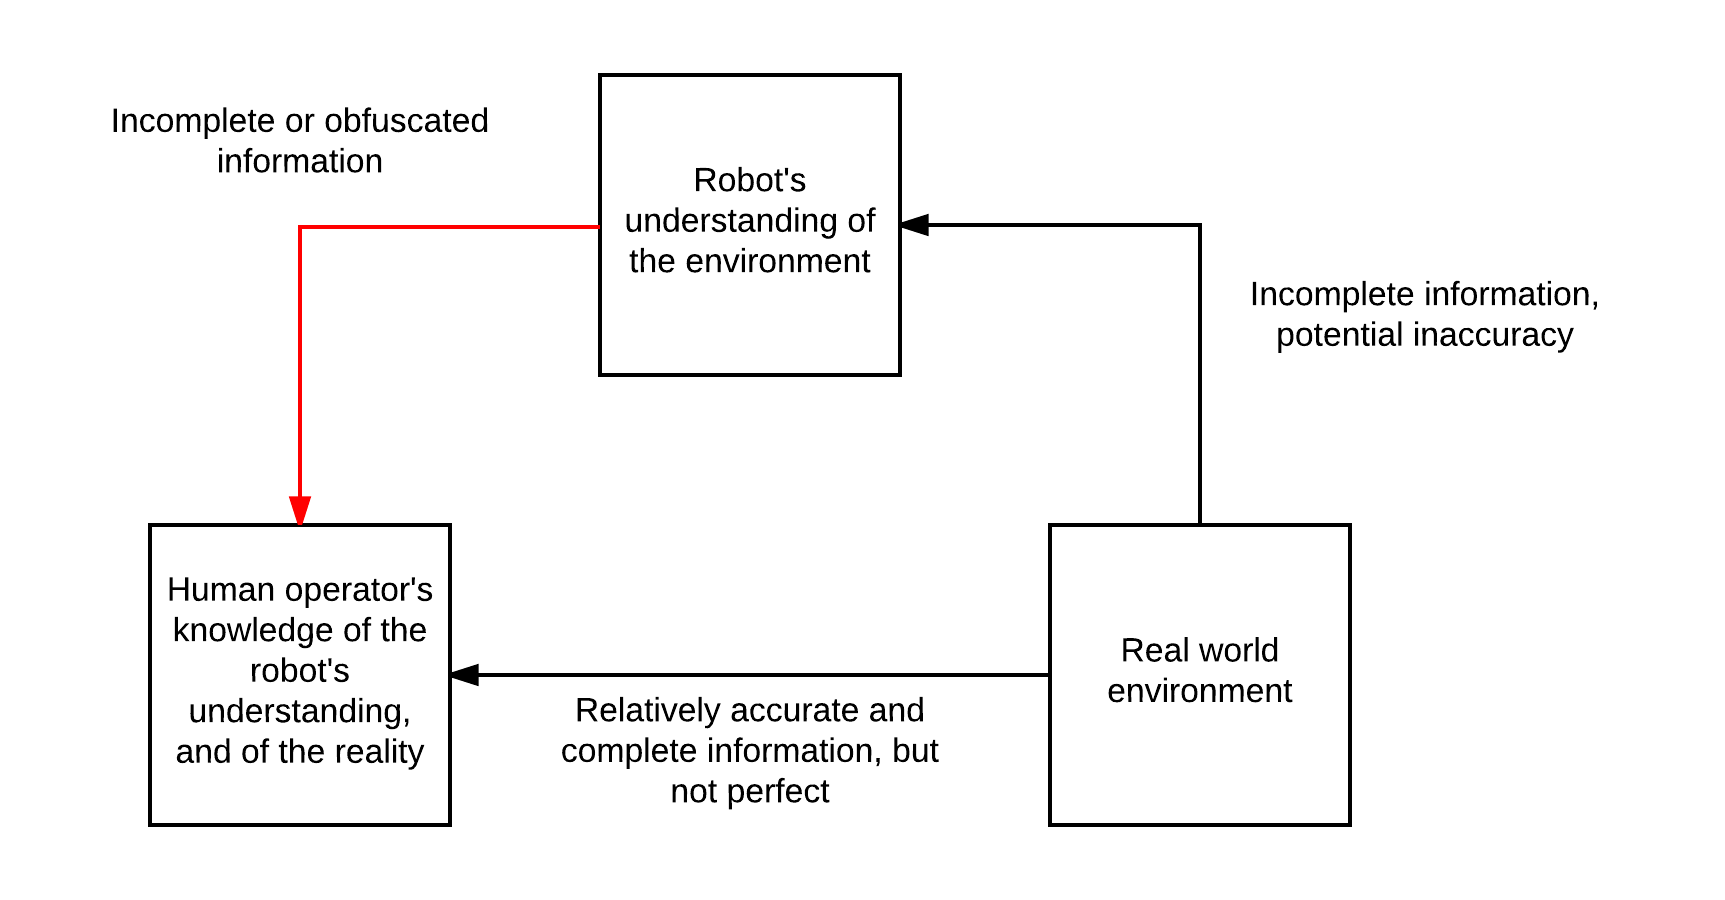
\includegraphics{Figures/RobotDebuggingInformationAbstraction.png}
	\decoRule
	\caption[Debugging Information]{Layers of information abstraction in robotics debugging.}
	\label{fig:DebuggingInformation}
\end{figure}

%----------------------------------------------------------------------------------------

\section{Project Concept} \label{ProjectConcept}
This project focuses on mitigating the problems discussed in the previous section, thus improving the timeliness with which bugs identified in a swarm robotics system can be located and fixed, by improving the operator's access to system information. This means collecting information from multiple sources and presenting it all in one place, in a human readable manner, in real time. The information sources to be used include the individual robots themselves, as well as a live camera feed of the robots' environment.

This project attempts to achieve this by creating a software application and associated wireless data transaction format to present a user with a single, coherent, and highly readable interface through which they can view relevant information about the swarm and it's constituent robots in real time. This includes the use of a video based tracking system to monitor robot positions, and provide the user with a view of the robots' environment. This can then be augmented with graphical representations of relevant elements of the data retrieved from the robots, such as sensor readings. The robots will communicate data to the computer running the application wirelessly. The wireless protocol to be used initially will be WiFi, with Bluetooth to be considered as a possible extension. The initial target robot platform is the widely used \textit{e-puck} robot [!!EPUCK REF!!], equipped with a Linux extension board and WiFi adapter, hence the choice of WiFi as the first wireless protocol to support. The e-puck platform is discussed in greater detail in section . The diagram in Figure  gives a logical representation of the proposed system architecture, in terms of its components, including the e-puck robots, tracking camera, and the application's host computer. This report describes the design, implementation and testing of this system, and includes details of the steps undertaken to evaluate its effectiveness. Some portions of this report appeared previously in a similar form in an \textit{Initial Report}, and are included here for completeness, with minor alterations.

\begin{figure}
	\begin{center}
	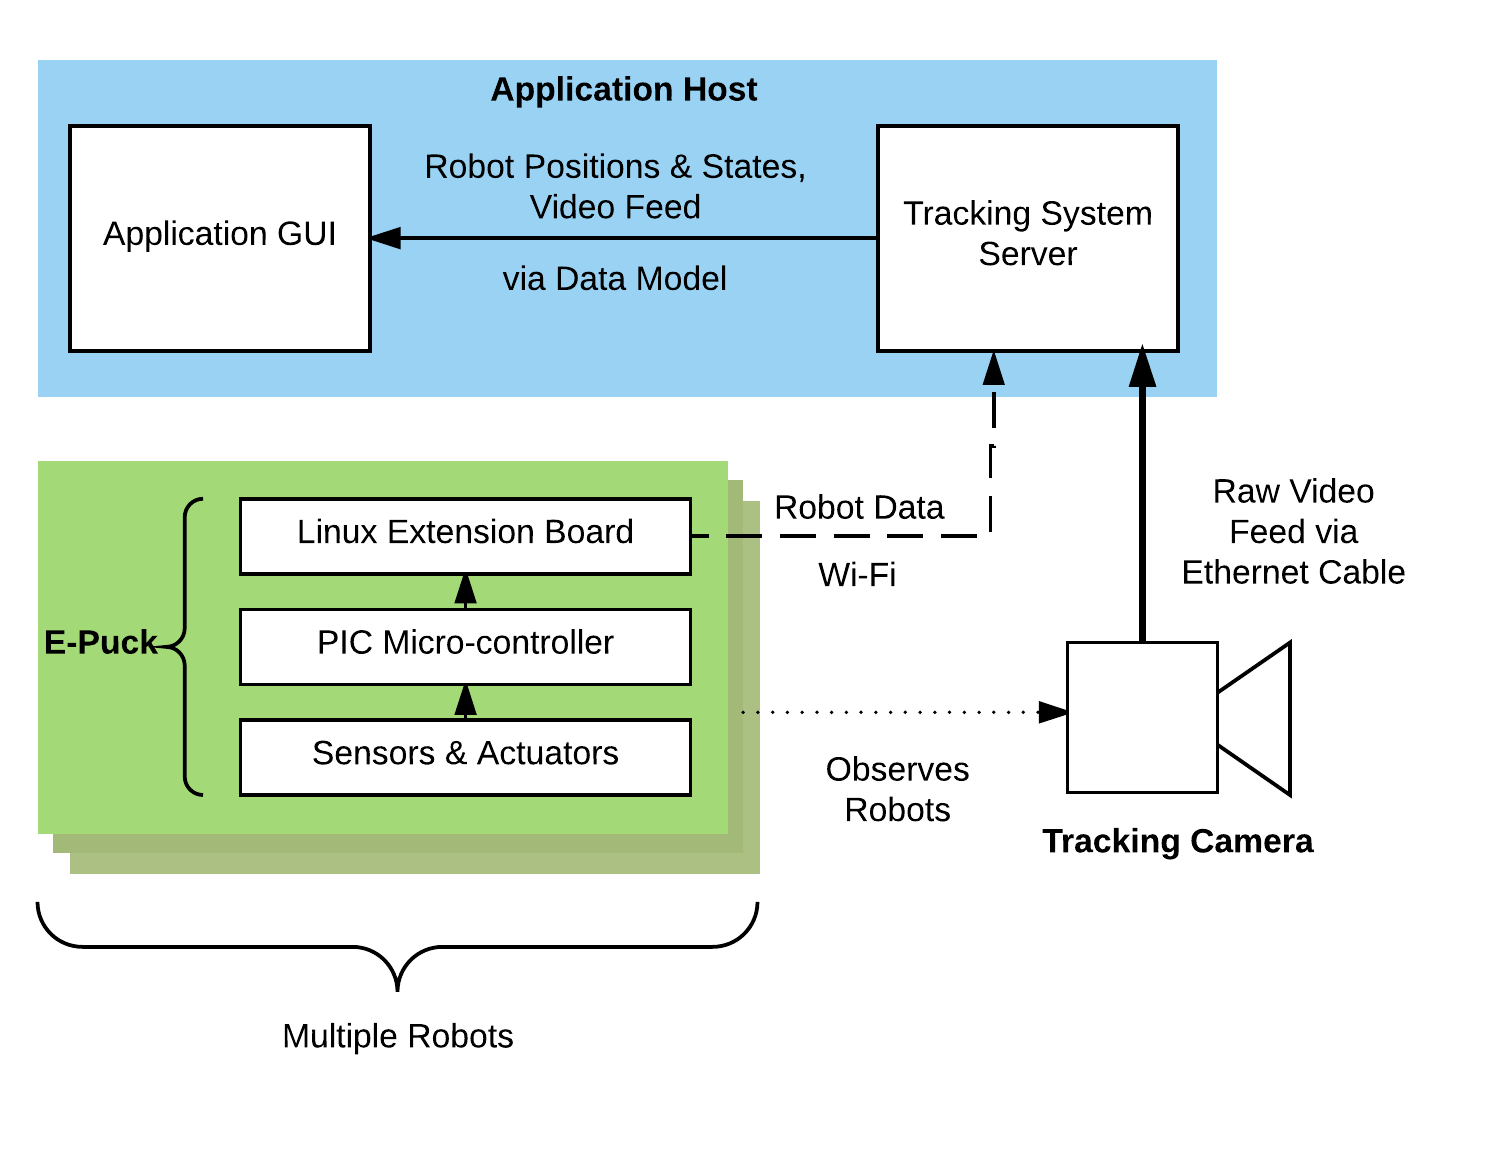
\includegraphics[scale=0.8]{SystemArchitecture.png}
	\decoRule
	\caption{The proposed system architecture.}
	\label{fig:SystemArchitecture}
	\end{center}
\end{figure}

%----------------------------------------------------------------------------------------

\section{Aim and Objectives}
Given the descriptions of the project context and concept in sections \ref{ProjectContext} and \ref{ProjectConcept}, the project aim can be formalised, and a set of objectives determined. This project aims to understand the needs of a swarm robotics researcher or system developer when attempting to debug their system, and create a computer application which allows a user to monitor the state and behaviour of a robot swarm system in real time, thus improving the ease and efficiency of this debugging process. The objectives required to achieve this aim are as follows:

\begin{itemize}
	\item Utilize existing fiducial marker based tracking technology to track the position of individual robots within a swarm over time.
	\item Develop code for presenting the user with a live video feed of a robot swarm, augmented with relevant and spatially situated information relating to the robots, using the data obtained from the tracking system.
	\item Develop code to allow multiple robots to communicate information regarding their internal state, sensor readings and decision making to the main application wirelessly via a network.
	\item Develop a data model that allows the application to store the information it receives from the robots, and update it as new information arrives.
	\item Develop code to ascertain higher level data related to the robots, such as recent movement history or state trasition history, and add this data to the model.
	\item Design and implement a user interface which presents the data model to the user in a human readable manner, and performs data fusion on the information provided by the robots and the tracking information.
	\item Develop the user interface in such a way as to allow the user to filter out information that is not currently relevant, and to contrast and compare information related to specific robots.
	\item Design and implement the system in a modular way so as to allow for relatively simple integration with other swarm robotic platforms and tracking systems in future extensions.
\end{itemize}

%----------------------------------------------------------------------------------------

\section{Functional Specification}
When developing software of any kind it is common practice to define a software specification prior to starting development. This specification describes the functionality required in the software in order for it to satisfy its purpose. The specification presented here is separated into core and secondary requirements. Core requirements are considered essential to the satisfactory delivery of the software. Secondary requirements will be satisfied where possible, given the time constraints of the project.

\textbf{Core Requirements:}
\begin{enumerate}
	\item Must be comprised of a PC application.
	\item Must be capable of receiving data related to the state of multiple robots.
	\item Must be capable of receiving positional data for the same set of robots.
	\item Must be capable of receiving a live video feed of the robots in their environment.
	\item Must collate received data and present it to the user in a combined graphical form.
	\item Must present auxiliary, non-spatial data to the user in textual or other forms.
	\item Must update in approximately real time.
	\item Must at minimum support the e-puck robot platform.
\end{enumerate}

\textbf{Secondary Requirements:}
\begin{enumerate}
	\item Should use a modularised structure.
	\item Should exchange data between the robot platform and the application using a platform-agnostic, extensible protocol.
	\item Should provide a basis for interoperability with a number of robotics platforms.
	\item Should allow the user to configure the displayed data.
	\item Should employ a model-view-controller (MVC) software architecture.
	\item Could provide the user with ways to configure and display custom data types.
	\item Could allow the user to compare data on two or more specific individual robots.
	\item Could calculate and display swarm-level meta-data and statistics.
	\item Could generate log files of robot activity over a user defined period.
\end{enumerate}

% Chapter 2

\chapter[Literature Review]{Literature Review} % Main chapter title

\label{Chapter2} % For referencing the chapter elsewhere, use \ref{Chapter1} 

%----------------------------------------------------------------------------------------

\section{Overview}
This section presents a review of some of the literature from the field of swarm robotics, beginning with some general summaries of the field's fundamentals, followed by a number of specific pieces of research from topic areas with particular relevance to this project. These areas include human-swarm interaction, robotics debugging, and robotics-focused augmented reality research. Finally a number of papers which connect augmented reality techniques directly to swarm robotics, and are therefore well aligned with the aims of this project, are discussed and critiqued. The results of this literature survey informed the project direction significantly, and formed the basis for many of the design and implementation decisions made later on. This literature review is also presented with the aim of providing the reader with the base of knowledge required to better understand the project.

%----------------------------------------------------------------------------------------

\section{Swarm Intelligence and Swarm Robotics} \label{GeneralSwarmRobotics}
An understanding of the fundamental concepts of Swarm Robotics, and to a lesser extent Swarm Intelligence, was deemed key to producing an application that is useful in practice, and will help a reader to better understand the purpose and aims of the project. A deep understanding of the technical details of specific swarm behaviours or implementations is not a priority for understanding this project, as the application aims to be more broadly applicable to a wide range of swarm systems. Emphasis has instead been placed on understanding the general classification of swarm robotic systems, relevant problem domains, and recurring concepts, so that the system might better serve researchers in the field.

Sahin \cite{Sahin:2004} presents a summary of the key concepts of swarm robotics, and attempts to offer a coherent description of the topic. He notes that a key difference from other multi-robot systems is the lack of centralised control, and the idea that desired swarm level behaviour should emerge from simple local interactions between robots, and between the robots and their environment. He also notes some of the key motivators behind Swarm Robotics research, stating that a swarm robotics system would ideally exhibit ``\textit{robustness}'', ``\textit{flexibility}'' and ``\textit{scalability}'' \cite{Sahin:2004}. 

Robustness refers to the swarm's ability to continue to function should one or more individual swarm members suffer a failure of some kind. Flexibility refers to the swarm's ability to adapt to changes in the environment without the need for re-programming. Scalability describes the idea that a swarm should be functional at a range of sizes, and that ideally the number of robots in the swarm could be increased or decreased depending on the demands of the task. These descriptors should be taken into account by the design of the system presented in this project. In order for the system to be able to work well with robust, scalable swarms it should adapt easily to variation in the number of robots being monitored. Newly detected robots should therefore be incorporated seamlessly. The video feed component of the system will allow a user to see the environment the swarm is interacting with and observe how robots respond to changes within it, and therefore judge the extent to which the swarm exhibits flexibility.

Sahin \cite{Sahin:2004} goes on to describe several classes of application for which Swarm Robotics systems might be well suited. Tasks that cover a region could benefit from a swarm's ability to distribute physically in a space according to need. Dangerous tasks could benefit from the relative dispensability of individual robots in the swarm; should one be damaged or destroyed the swarm could continue to function, and it would be less costly than the loss of a single, complex, expensive robot. Tasks requiring scalability are good candidates, as discussed before, and tasks that require redundancy are also highlighted, as swarm systems should have the ability to degrade gracefully, rather than suffering a single catastrophic failure. Through this generalisation of the application areas, insight can be gained into the kinds of work swarm robotics researchers are likely to be doing, and this should inform the design of the application. Overall Sahin's paper \cite{Sahin:2004} provides a coherent, succinct overview of the field, and although it is now over a decade old the concepts covered remain relevant.

The book `\textit{Swarm Intelligence: From Natural to Artificial Systems}', by Bonabeau, Dorigo and Theraulaz \cite{Bonabeau:1999}, provides in its introductory chapter a good overview of the biological concepts and animal behaviours which inspired much of the research that led to the creation of the field of swarm intelligence. Fundamental concepts such as self-organisation and decentralised control are discussed. In order to be a useful tool in the swarm robotics research space, it is important that the system developed during this project does not violate these core principles of the swarm robotics paradigm. Therefore the system should not facilitate low level control of the robots or allow for forms of communication and data exchange that might invalidate the self-organising, decentralised nature of the swarm's behaviour. 

\begin{figure}
 \begin{center}
 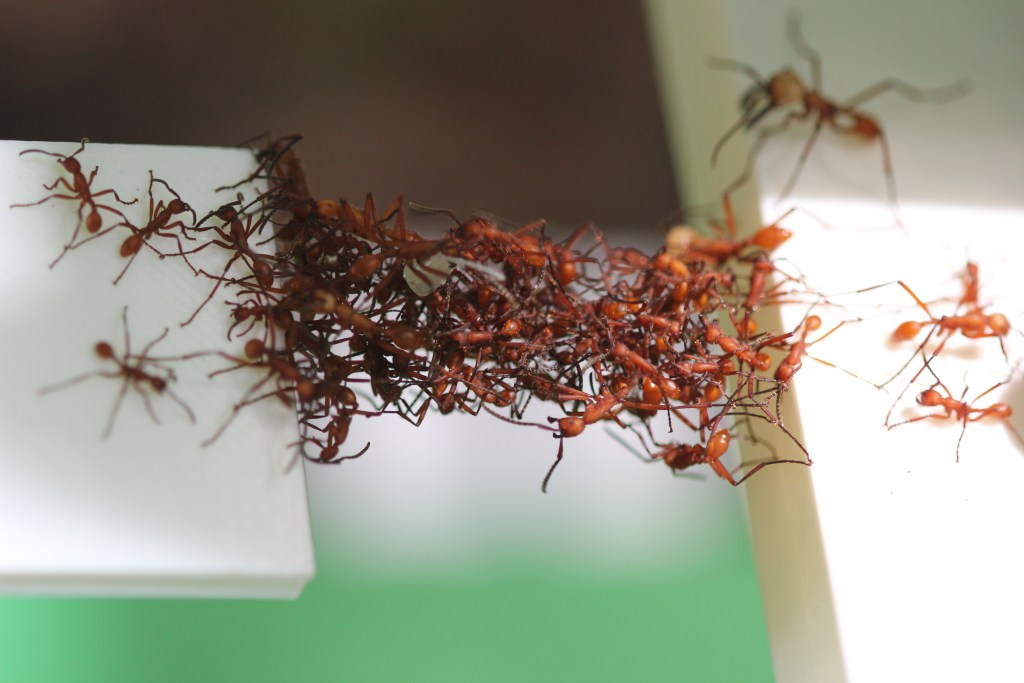
\includegraphics[width=\textwidth]{AntBridge.png}
 \decoRule
 \caption[Army Ants Bridging a Gap \cite{AntBridge}.]{A swarm of army ants forming a living bridge to cross a gap \cite{AntBridge}.}
 \label{fig:AntBridge}
 \end{center}
\end{figure}

The later chapters \cite{Bonabeau:1999} provide a detailed look at several key insect behaviours, and how mathematical models and algorithms can be derived to mimic them. An understanding of these behaviours and models can offer insight into what information the application might need to expose to allow a user to validate the correct operation of a swarm behaviour based on these concepts. A number of these algorithms focus or rely on data related to the position and movement of individuals within the swarm, and the swarm as a whole. The system developed during this project should reflect the importance of positional data and provide features which aid the user in interpreting it.

In a more modern work, Brambilla et al. \cite{Brambilla:2013} focus heavily on the engineering practicalities of designing, implementing and testing swarm robotic systems. The authors then apply this focus as a means by which to classify and critique a large body of swarm robotics research, noting that although much work has been carried out regarding the design and analysis of swarm behaviours, other areas including maintenance and performance measurement are heavily lacking in research contributions \cite{Brambilla:2013}. Debugging can be considered a maintenance task, and the system developed in this project has potential in both maintenance and performance measurement applications. It is hoped therefore that this work might contribute to this area of the field, by investigating through implementation the practicalities of a generalised swarm maintenance and observation software application. The authors \cite{Brambilla:2013} later note that human-swarm interaction remains an open issue, and will be key to realising functional, real-world swarm robotic systems. They identify a number of works related to human-swarm interaction, almost all of which focus on the task of controlling a robot swarm, and investigate different methods by which a user might insert data into the swarm system. Little consideration appears to be given, both in this paper and throughout the literature, to the task of monitoring a swarm, and best practices for retrieving information in a manner that is useful to a human operator.

%----------------------------------------------------------------------------------------

\section{Human Swarm Interaction} \label{HumanSwarmInteraction}
This project focuses on a piece of software which forms an interface between a human operator and a robot swarm. A relevant area of research is therefore Human-Swarm Interaction (HSI). Research in this area focuses on the different ways in which humans and robot swarms can interact, the different roles humans take whilst interacting with robot swarms, and the best practices for facilitating this interaction given different aims, and different user roles (developer, researcher, end user, etc.). The two key challenges of HSI are \textit{control} and \textit{monitoring}. The former refers to how best to allow a human operator to direct the behaviour of a decentralised swarm, whilst the latter refers to how best to retrieve data from a swarm and present it in a useful, human readable manner. This project is related to debugging robot swarm behaviours, which is primarily a swarm monitoring task, and therefore this section focuses on the monitoring side of HSI.

In their paper `\textit{Human Interaction with Robot Swarms: A Survey}' \cite{Kolling:2016} Kolling at el. begin by noting the lack of research into methods for interfacing humans and robot swarms. They suggest that real-world applications for swarm robotics systems are now within reach, and that discovering effective methods for allowing humans to control and/or supervise swarms is a key barrier to realising these systems. The paper \cite{Kolling:2016} provides a detailed analysis of human swarm interaction from a number of different perspectives. Of relevance to this project is the statement on page 15 that ``\textit{Proper supervision of a semiautonomous swarm requires the human operator to be able to observe the state and motion of the swarm, as well as predict its future state to within some reasonable accuracy}'' \cite{Kolling:2016}. This statement lends credence to the aims of this project, as swarm supervision and swarm debugging are highly comparable tasks; both involve observing the swarm whilst performing its task and determining the validity of the behaviour observed. The system developed in this project should allow the state of the swarm, including the internal state of individual robots, to be observed simultaneously with the physical positions and motions of the robots within their environment. The paper \cite{Kolling:2016} goes on to suggest that by observing the swarm over time the human operator will be able to provide `\textit{appropriate control inputs}'. In the case of this application, rather than providing control input, the human operator will be seeking to identify faults, and provide appropriate corrections to the system, however the concept of state visualisation remains relevant.

Rule and Forlizzi \cite{Rule:2012} present a thorough examination of the complexities of human robot interaction (HRI) when dealing with multi-robot (and multi-user) systems. Much of the paper focusses on control methods, which are not directly applicable to this project, however section 2.4 titled \textit{Salience of Information} discusses the task of designing interfaces for displaying information about multi-robot systems to a human operator in a manner which is both information dense and rapidly understandable. The authors note that the use of colour has been shown to improve interface readability \cite{Christ:1984}, and that the brain has been shown to process text faster than images \cite{Carney:1998}, hence complex icons should be avoided. These ideas should be incorporated into the design of the application user interface for this project. A range of different designs could be explored, including finding a balance between the amount of information displayed graphically, and the amount displayed textually, and deciding whether to use colour to differentiate between individual robots, or to differentiate between different types of data, or a combination of both.

The authors \cite{Rule:2012} then go on to use `\textit{contextual inquiry}' interviews with robot operators to determine a set of questions which, if answered, should allow for robust robot operation. Of relevance to this project are the four questions in the \textit{human-robot} category. These are 1) ``\textit{What mode, state, and environment is the robot in and how will this affect my commands?}'', 2) ``\textit{Which robot needs my attention?}'', 3) ``\textit{What is each robot accomplishing?}'', and 4) ``\textit{What can I accomplish with this robot?}''. Providing the user with answers to questions two, three and four is beyond the scope of this project, however the system should provide the user with an answer to question one, by allowing access to state and environment information simultaneously. 

Once again although the authors \cite{Rule:2012} consider only a robot control perspective, these questions remain broadly relevant to a debugging perspective also. For example, question one could be rephrased as \textit{What mode, state, and environment is the robot in, and is this having the correct effect on its behaviour?} to better fit the use case of this project. When discussing the appropriate level of display salience for robot state awareness in section 4.8 \cite{Rule:2012}, the authors note that users wanted the ability to ``\textit{select which aspects of robot information to view at any one time}''. They also state that users wanted basic overview information, with the ability to access a more detailed view specific to one robot when ``troubleshooting''. This configurable, layered approach to information display and access should be incorporated into the user interface design for the system.

The authors \cite{Rule:2012} do not state how they determined that the set of situation awareness questions presented ensure robustness. The contextual inquiry method is potentially subjective, suggesting that answering only these questions may not guarantee full awareness. Other factors which a system user could benefit from an awareness of should be considered. For example the authors mention the robot's mode, state and environment, but do not include the robot's sensor data. Furthermore care must be taken when applying the results of this work to swarm robotic systems, as it was not produced with swarms specifically in mind. Therefore applying the results within, without also considering needs specific to swarm robotics, could lead to too strong a focus on the actions of individual robots, and a lack of focus on the overall behaviour of the swarm.

Podevijn, O'Grady and Dorigo \cite{Podevijn:2012} present a novel method for obtaining feedback from an active robot swarm. The authors propose that information sent back from a self-organised swarm to an operator should itself be self-organised. They note a number of motivations for this approach. Firstly, should every robot simultaneously report information regarding its own ``\textit{local worldview}'', the authors suggest \cite{Podevijn:2012} that the operator would be over-burdened with an excess of information, and would therefore need further tools of some kind to parse this data effectively. They also suggest that the required communication infrastructure would increase the overall system complexity, and the hardware requirements of each robot. The volume of communication traffic for a large swarm might also prove impossible for a network to handle. 

Their work \cite{Podevijn:2012} demonstrates a number of possible methods by which a swarm of robots might report information in a self organised manner, in the hope of combining and reducing the information that needs to be reported. Whilst completing a grouping task, coloured LEDs were used to indicate visually which group each robot was a part of. This can be seen in figure \ref{fig:SelfOrganisedFeedback}. Another proposed mechanism \cite{Podevijn:2012} would use the formation of the swarm to indicate information about their behaviour, for example when moving collectively in one direction the robots would arrange into an arrow formation indicating the direction of movement. This mechanism was proposed only in concept, and not implemented on a real swarm.

\begin{figure}
 \begin{center}
 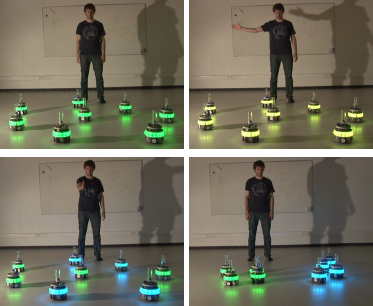
\includegraphics[scale=1]{SelfOrganisedFeedback.png}
 \decoRule
 \caption[Self Organised Feedback \cite{Podevijn:2012}.]{Self-organised, colour-based feedback during a selection and grouping task \cite{Podevijn:2012}. }
 \label{fig:SelfOrganisedFeedback}
 \end{center}
\end{figure}

This self organised approach to information reporting \cite{Podevijn:2012} has a number of issues. Firstly, the additional behaviour required to report information in a self organised manner may negatively impact the original desired behaviour of the swarm. In the case of the arrow formation example, having the robots move into a readable formation might disrupt other position-based behaviour. Implementing these information-reporting behaviours might also add significant complexity to the robots behavioural code, further increasing the difficulty of the already complex task of implementing a swarm behaviour. Furthermore, from a debugging perspective, this kind of high level, aggregate data reporting does not allow access to the low level internal state information that can be essential to isolating the cause of an observed issue.

The communication infrastructure requirements of a system that allows a large number of robots to communicate individually with the host are a concern, however in practice robot swarms tend to be composed of numbers of robots which are not unmanageable given modern networking technology. Standard WiFi networks are capable of supporting relatively high numbers of connected devices, whilst developments in mesh-network technologies driven by the emerging Internet of Things sector have made it possible for networks of very large numbers of devices to be achieved with relatively modest hardware \cite{Nguyen:2012}. In addition, the complexity increase due to greater networking and communication requirements is a known quantity; these technologies already exist and have standardised implementations. In contrast, implementing additional swarm behaviours to report information adds unknown complexity, as a reliable, formalised method for developing arbitrary swarm behaviours is still an open problem.

Finally the authors' assertion that the volume of data received from a swarm of individually reporting robots would overwhelm an operator is potentially true. However, a centralised host receiving all of the reported data is far better positioned than the swarm itself to process and condense this information into a form that the user can handle, without sacrificing on detail. This can also provide the user with access to variable levels of information, giving them greater control overall. In summary the concept of self-organised feedback as presented in \cite{Podevijn:2012} shows promise for situations where relatively simple, high level information is required to be directly apparent to a system user. However in practice the added complexity at the behavioural level, and the potential to interfere with other desired behaviour, may well outweigh the benefits of reduced communications complexity and infrastructure. By creating a generalised platform for swarm robot information reporting, this project could establish communications infrastructure requirements as a known, fixed quantity, which can potentially be re-used across multiple swarms.

McLurkin et al. \cite{McLurkin:2006} discuss the practical considerations of interfacing a human operator with their large swarm of 112 robots. The relevant portion of this work discusses the use of ``\textit{utility software for centralised development and debugging}'' \cite{McLurkin:2006}. The authors note the success of graphical interfaces based on those found in \textit{Real Time Strategy} video games for centralised data collection and display. Their \textit{SwarmCraft} graphical user interface (GUI), shown in figure \ref{fig:SwarmCraft}, can display information received regarding individuals, groups, or the whole swarm in a number of graphical forms. The authors \cite{McLurkin:2006} note that one potential issue is keeping the code for displaying the data and the code on the robot side in sync, such that the GUI can always correctly display the received data. The idea of a standardised data transfer format investigated by this project could provide a potential solution to this issue.

The authors \cite{McLurkin:2006} go on to discuss the problem of using monitors to display the robots' internal state information when debugging group behaviours, as a user must continuously switch between watching the swarm and looking at the monitor for detailed information. The authors use a `global output' system of LEDs and sounds to solve this issue. This output is however inherently limited by the amount of information that can be represented using the small number of LEDs, and the quality of information acquired from a swarm of robots all generating sound at once. This approach also requires specific hardware to be present on each of the robots, such as the LEDs and a speaker. Augmented reality (AR) techniques therefore offer a potentially more powerful solution; by superimposing the information that would traditionally be found by looking at the monitor onto a view of the robots themselves, the user can access all available information without looking away from the swarm's activity. Furthermore the requirement for the global output hardware is removed, and the user does not need to learn how to correctly interpret these somewhat cryptic output systems, as an AR solution could display information in any form necessary, including text.

\begin{figure}
 \begin{center}
 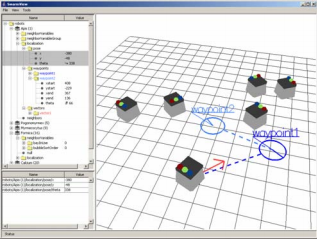
\includegraphics[scale=1]{SwarmCraft.png}
 \decoRule
 \caption[Swarm Craft GUI \cite{McLurkin:2006}.]{A screenshot of the \textit{SwarmCraft} GUI, developed by McLurkin et al. \cite{McLurkin:2006}.}
 \label{fig:SwarmCraft}
 \end{center}
\end{figure}

%----------------------------------------------------------------------------------------

\section{Robotics Debugging} \label{RoboticsDebugging}
`\textit{Debugging}' is the name given to the process of fixing problems or issues (commonly referred to as bugs) in a piece of software. Well established tool-sets and techniques exist for debugging traditional software, however debugging robotic systems is a fundamentally different and more complex problem, as discussed in section \ref{ProjectContext}. The literature reviewed in this section examines the challenges of robotics debugging, and presents some tools and techniques for reducing the difficulty of this task.

Collet and MacDonald \cite{Collet:2006} describe in detail the difficulties in debugging robotics systems. The authors identify that the difficulties in developing and debugging robotics applications when compared to traditional software arise from either the environment of the robot - which will often be ``\textit{uncontrolled}'' and ``\textit{dynamic}'' - or from the mobile nature of the robot. Because the environment a given robot operates in is a real world space, the level of control that can be exerted over it by the researcher or operator is inherently limited \cite{Collet:2006}. The environment may therefore change over time, exhibit imperfections, and include other time-varying elements. A robot is a physical actor and will likely experience dynamic change in its sensor readings and its relationship to the environment over time. This is especially true for mobile robots, whose position and orientation will change over time. The behaviour of the robot often largely depends on these highly variable factors, and therefore replicating a given behaviour exactly becomes almost impossible. 

The authors go on to state that difficulties in debugging often arise from ``\textit{the programmer's lack of understanding of the robot's world view} \cite{Collet:2006}''. It can therefore be extrapolated that for a multi robot system such as a robot swarm this problem would be exacerbated. Each robot will have its own perception of the environment, which will differ based on differences in the robots' positions and orientations as well as variations in the instrumentation of each robot. For a multi-robot system the programmer is required to have an understanding of not just one but multiple world views, adding yet more potential for error and inaccuracy, and further obscuring bugs or behavioural issues that the programmer is trying to diagnose. This work \cite{Collet:2006} suggests that developers will need specific tools which enhance their understanding of the robots' world view in order to develop effectively for swarm robotic platforms. This need forms the mandate for the majority of this project. Collet and MacDonald \cite{Collet:2006} go on to discuss the use of augmented reality to satisfy this need, and present an augmented reality based software tool for this purpose, which is discussed in Section \ref{AugmentedReality}.

Gumbley and MacDonald \cite{Gumbley:2009} identify one of the core issues in debugging robotic behaviours using traditional debugging software to be the assumption of a ``\textit{deterministic, suspendable environment}''. This assumption rarely holds true for robots, due to their existence in a real world environment. The authors note that traditional debugging constructs such as breakpoints pause code execution, but cannot for obvious reasons also pause a robot's environment. This allows the robot's environment to change whilst execution is paused, therefore affecting the robot's behaviour. In the case where a breakpoint has been inserted to try to isolate the cause of a previously observed fault, this change in behaviour may also stop the fault from occurring. The authors \cite{Gumbley:2009} go on to consider a number of possible methods by which a developer can obtain information without pausing execution, including live data extraction which is the method chosen in this project. They note that adding code to extract information without pausing execution has the potential to affect robot behaviour. This is a salient point, and should be considered when implementing the robot-side portion of this project, where care must be taken to minimise the affect data reporting has on the execution of the robot's actual behaviour. Issues of this nature could be caused by the data reporting code taking too long to execute, thus disrupting robot behaviour. Keeping the data reporting code lightweight and efficient should therefore be a priority.

\begin{figure}
 \begin{center}
 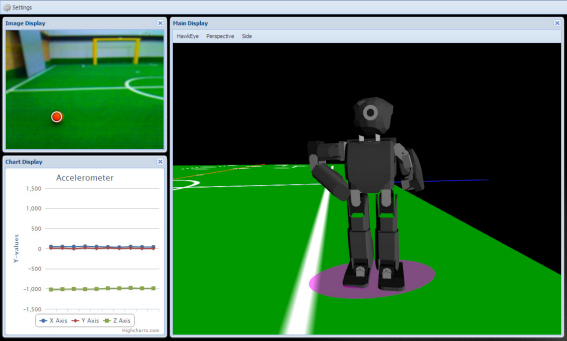
\includegraphics[scale=0.8]{NUbugger.png}
 \decoRule
 \caption[\textit{NUbugger} GUI \cite{Annable:2014}.]{The \textit{NUbugger} GUI, a real time, visual, robotics debugging utility developed by Annable et al. \cite{Annable:2014}.}
 \label{fig:NUbugger}
 \end{center}
\end{figure}

In their `\textit{NUbugger}' system \cite{Annable:2014}, Annable, Budden and Mendes implement a real time, visual debugging system for robotics. The authors begin by noting that the continually increasing complexity of robotic hardware and software has lead to typical debugging approaches based on diagnosis via observation of high-level symptoms becoming increasingly less useful. They note the need for real time, visual tools, to reflect the active, physical nature of robots. The authors system \cite{Annable:2014} streams all critical system information from their robot to a web server in real time, where it can be viewed in a graphical client. The graphical interface, shown in figure \ref{fig:NUbugger}, includes a visualisation of the humanoid robot position, orientation and pose, based on its own self-localisation belief and servomotor sensor readings. It also includes a live feed from the robot's built in camera, and graphs of real time sensor data. 

The system has been used to diagnose a number of real, low-level issues \cite{Annable:2014} relating to the robot's image processing and object detection functionalities, demonstrating the effectiveness of real time, visual debugging tools. The use of a web server in the authors' implementation \cite{Annable:2014} allows for the collection of information regarding multiple robots, and the display of this information in multiple clients, making the system highly versatile. However one possible limitation introduced as a result is the need for a number of relatively complex networking libraries to be running on the robots, and a high connection bandwidth, in order to send the required information, limiting the system to use on relatively complex, high performance robot platforms. The system is also only targeted at a single robot platform.

%----------------------------------------------------------------------------------------

\section{Augmented Reality and Single-Robot Systems} \label{AugmentedReality}

\begin{figure}[h]
	\centering
	\makebox[\textwidth][c]{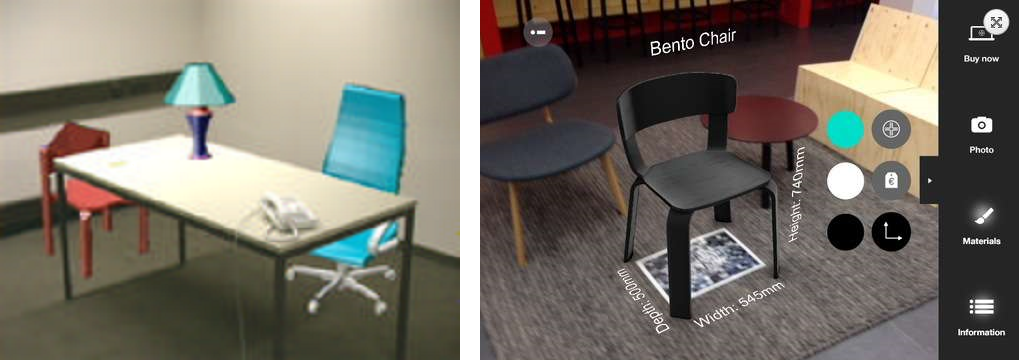
\includegraphics[width=\textwidth]{ARDouble.png}}
	\decoRule
	\caption[AR Furniture Visualisations \cite{Azuma:1997} \cite{SayDuck}.]{Left: An early example of an AR lamp and chairs augmenting a real table \cite{Azuma:1997}. Right: A modern furniture visualisation app, showing a virtual chair \cite{SayDuck}.}
	\label{fig:ARFurniture}
\end{figure}

Augmented Reality (AR) is the term used to describe the process of super-imposing `virtual' objects and elements, in the form of computer generated graphics, on to a live video image of the real world \cite{Azuma:1997}. The general aim of any augmented reality system is to give the impression that the virtual objects being rendered are actually situated within the user's real environment, and to allow the user to interact with them as such. True AR is sometimes defined as requiring the use of a \textit{head-mounted display} (HMD), as this leads to much more immersive qualities akin to virtual reality, to which AR is closely related. However this is not a universal requirement, and in one of the most widely cited surveys of the topic, Azuma \cite{Azuma:1997} provides a definition which states only three requirements of an AR system; the combination of virtual and real content, real time interaction, and 3D rendering. Figure \ref{fig:ARFurniture} shows on the left the example image used in Azuma's \cite{Azuma:1997} survey. It includes a view of a real table, augmented by virtual furniture. On the right is a modern example from a furniture testing app \cite{SayDuck}.

Augmented reality presents a powerful tool for debugging robots as it allows information gathered by a robot about an environment to be superimposed onto a real world view of that environment, such that discrepancies and inconsistencies between this information and the real world become inherently obvious. More generally, augmented reality can be used to create a shared space between a human and a robot. Even as early as 1997, Azuma \cite{Azuma:1997} notes that augmented reality has a potential application in robot path planning. One limitation of Azuma's survey is its age, as the two decades since its publication have seen rapid development in computing power and computer graphics, as well as augmented reality hardware. High fidelity, consumer HMDs, such as the \textit{Microsoft HoloLens} \cite{MicrosoftHoloLens} shown in figure \ref{fig:HoloLens}, have been beginning to emerge into use within real world applications since the mid-to-late 2010s \cite{HoloLens}. A more recent survey of the topic from 2014 \cite{Billinghurst:2014} agrees with many of Azuma's earlier definitions, but provides many examples of new applications of AR technologies. The author notes the power of AR as a new paradigm for human computer interaction, and the wealth of potential application areas, including robotics.

\begin{figure}
	\begin{center}
	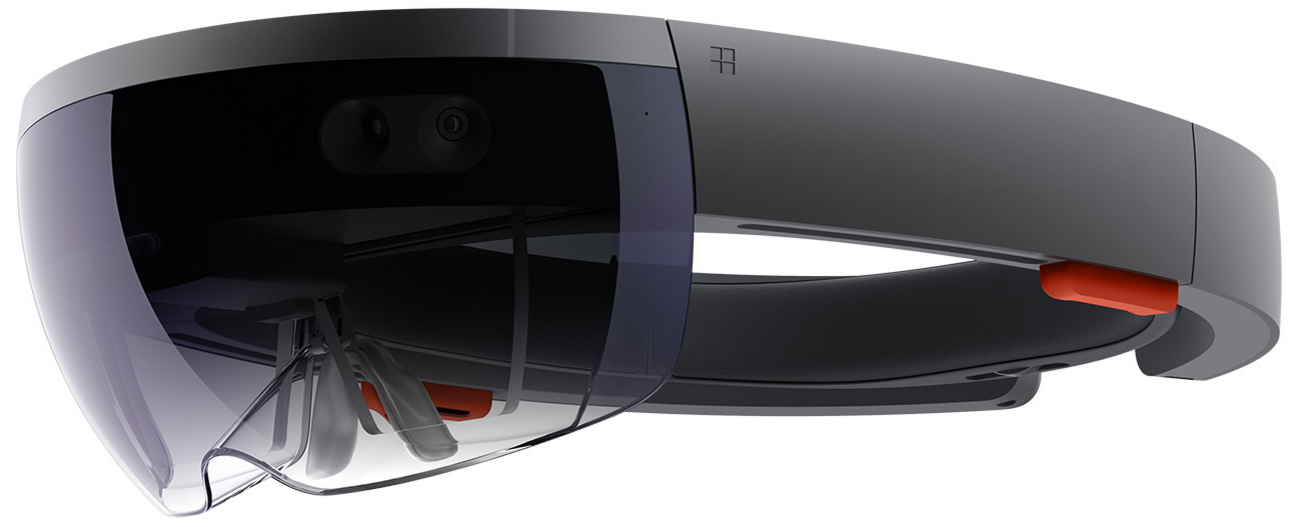
\includegraphics[scale=0.4]{HoloLens.png}
	\decoRule
	\caption[Microsoft HoloLens \cite{MicrosoftHoloLens}]{The Microsoft HoloLens head mounted display \cite{MicrosoftHoloLens}.}
	\label{fig:HoloLens}
	\end{center}
\end{figure}

Milgram et al. \cite{Milgram:1993} discuss the different communication formats used to interface between humans and robots, grouping them into ``\textit{continuous}'' and ``\textit{discrete}'' formats. For any communication involving a spatial or temporal component, the process of converting to and from a discrete format in order to transmit this information is an unnecessary burden. Both humans and robots use the continuous spatial dimensions, and humans have an inherent, instinctive understanding of physical things expressed in three dimensions. The authors \cite{Milgram:1993} therefore identify that  augmented reality provides an excellent means of supporting the communication of spatial information. Their paper focuses on the combination of stereoscopic displays and computer generated graphics to allow for more intuitive control of robotic systems. In the case of this project the concept is reversed; robots reporting spatial information for validation by a user should do so in a format which is inherently continuous such as a graphical visualisation in AR, rather than one that is discrete such as text-based numerical output. This should in theory reduce the time required for a human to process the information. The authors note \cite{Milgram:1993} that the ideal system utilises both discrete and continuous formats where appropriate to best communicate the required information, and is ergonomically designed to allow the user to make use of both easily and intuitively.

Like much of the HSI literature surveyed, this paper \cite{Milgram:1993} is focused primarily on robot control, rather than observation and monitoring. In spite of this much of the content of the paper remains applicable. Since the paper was written, just over twenty five years ago, major advancements have been made in virtually every area mentioned, including the quality and precision of robotic systems, their cognitive, perceptive and decision making abilities, augmented reality technologies and robotic autonomy. Because of this, some of the content of the paper has fallen out of date. Specifically, the assumption that robots lack the level of autonomy required to survey their environment and then form and execute a series of steps to carry out a relatively high level task, such as ``find and go to object Q''\cite{Milgram:1993}, is no longer necessarily true. A number of modern robots possess sufficient sensing capabilities, processing power and cognitive programming to perform such tasks based on high level commands. This does not however devalue the AR methods discussed within, and given the increased complexity and sensing capabilities of modern robots, AR based methods of interaction actually have more potential than ever. The paper however makes no mention of the potential for an AR system to report data from a robot's sensors visually, which may be attributed to the technological limitations of the time rather than an oversight by the authors.

Collet and MacDonald \cite{Collet:2006} suggest that augmented reality tools can address and mitigate some of the robotics debugging issues discussed in section \ref{RoboticsDebugging} by superimposing graphical representations of the robot's understanding of the environment on top of a live view of the environment itself \cite{Collet:2006}. Hence the programmer is able to see how the robot has interpreted the environment, and identify inconsistencies. The authors describe the image of the real world environment as the ``\textit{ground truth}'' against which the robot's view can be compared and contrasted \cite{Collet:2006}. Figure \ref{fig:Sonar} shows a visual example of this technique, where the data received from the robot's sonar sensors is converted to spatially situated 3D shapes and superimposed over the live image, and can therefore be verified visually by the user.

\begin{figure}
	\begin{center}
	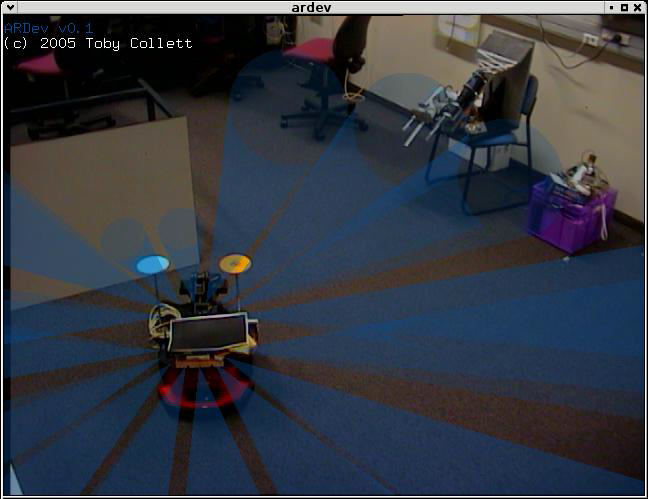
\includegraphics[scale=0.6]{Sonar.png}
	\decoRule
	\caption[Sonar data visualisation. Collet and MacDonald \cite{Collet:2006}]{Sonar sensor data visualisation in Collet and MacDonald's system \cite{Collet:2006}.}
	\label{fig:Sonar}
	\end{center}
\end{figure}

The application developed during this project closely follows this paradigm; allowing the user to identify bugs by comparing the robot's knowledge of its environment and its decision making factors (collectively referred to as its state) with a view of the environment, in real time. The application aims to apply this concept specifically to swarm robotics systems, and therefore must allow the user to compare the states of multiple robots with the environment simultaneously. From the perspective of each robot in the swarm, the other robots will form part of the environment, therefore the application must take this into account when displaying the information. Because of the large increase in information from a single-robot system to a multi-robot one, it becomes important that the application provides a way for the user to filter what information is displayed, allowing them to focus on the primary aspect under test. Filtering also allows the user to compare and contrast specific robots against one another by filtering out information related to other robots, or by displaying in more detail information related to the robots of interest.

\section{Augmented Reality and Multiple-Robot Systems} \label{SimilarWork}
A number of pieces of research have investigated different ways to monitor and interact with multi-robot systems, using a combination of augmented reality technology and HSI techniques. These similar works are summarised and reviewed in this section.

Daily et al. \cite{Daily:2003} present a technique for retrieving information from a swarm of robots, and displaying this to a user in a ``\textit{world-embedded}'' manner using augmented reality techniques. One of the stated aims of this work was the use of minimal communication bandwidth. The authors present \cite{Daily:2003} an infra-red (IR) LED based solution for both indicating robot position, and communicating a small amount of information, in the form of coded pulse sequences, simultaneously. The HMD worn by the user decodes this information and superimposes a graphical representation on top of the user's view of the robots using a see-through optical display. Communicating via IR LED directly to the user's HMD removes the need for communication infrastructure, however it requires the user to have a direct line-of-sight to the robots in order to receive information. The data rate that can be achieved via this method is also heavily limited. However in the use case demonstrated by the authors \cite{Daily:2003}, involving the display of a gradient in the direction of a target known to the swarm, the system is effective. The hardware requirements for this system are quite specific, and unlikely to be available on most robotics platforms, however the power of this kind of spatially situated or world-embedded data visualisation is clear.

Ghiringhelli et al. \cite{Ghiringhelli:2014} present a system for augmenting a video feed of an environment containing a number of robots with real time information obtained from each of the robots. This is similar in concept to the system described by Collet and MacDonald \cite{Collet:2006}, but is designed specifically to target a multi-robot system. The authors identify the ability to overlay spatial information exposed by the robots on to the video feed in real time, in the form of situated graphical representations, as the most important debugging feature of the system. Figure \ref{fig:SpatiallySituated} shows a spatially situated overlay of data exposed by robot thirty two, in the authors' system \cite{Ghiringhelli:2014}. A viewer is able to immediately verify the validity of the robot's world view from this image by comparing the blue overlay to the image beneath. Each robot features a coloured LED blinking a unique coded pattern to enable tracking, and the system uses homography techniques to map between each robot's frame of reference and the camera's \cite{Ghiringhelli:2014}. The author's system therefore requires hardware to be present on the robots to support the tracking method. The homography technique also requires a reference frame to be established on the floor of the robot space. 

The system developed in this project uses a simpler approach, with position and orientation tracking achieved through the use of the ArUco \cite{Garrido:2014} marker-based tracking system. The camera is positioned with a bird's-eye view of the space, to simplify mapping by effectively reducing the 3D space to a 2D approximation. The tracking LEDs used by the authors' system \cite{Ghiringhelli:2014} are active components, and therefore require specific hardware to be available on the robots in order for them to be tracked. This limits the system's generalisability. In contrast, using a passive, marker based technique means that no specific hardware is required, and the tracking could in theory be performed on any robot to which a marker can be attached.

\begin{figure}
	\begin{center}
	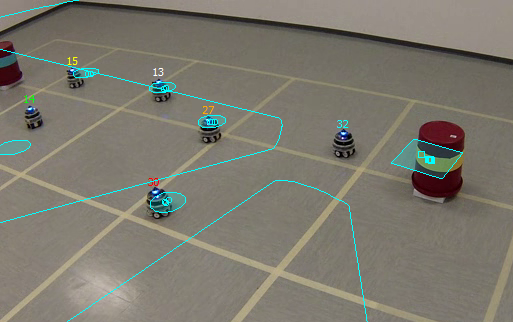
\includegraphics[scale=0.8]{SpatiallySituatedData.png}
	\decoRule
	\caption[Spatially situation data overlay. Garrido et al. \cite{Ghiringhelli:2014}]{Example of spatially situated data overlayed on a live image in \cite{Ghiringhelli:2014}.}
	\label{fig:SpatiallySituated}
	\end{center}
\end{figure}

The authors \cite{Ghiringhelli:2014} also note the inclusion of a number of interaction modalities which allow the user to manipulate the visibility and display of specific elements of the data, which is grouped according to its associated robot and its type. This allows a user to focus only on pertinent information by hiding other information which is irrelevant. This follows the guidelines established in Rule and Forlizzi's work \cite{Rule:2012} on HSI, and the requirements of users regarding information salience and display when interacting with multi robot systems. Following this precedent, display configuration was identified as a priority and implemented within the system described in this project. This project also looks at expanding the methods used to display data to include more standard interface elements not directly related to the video image, as previously seen in \cite{McLurkin:2006}, which is not addressed in \cite{Ghiringhelli:2014}. Overall Ghiringhelli et al. \cite{Ghiringhelli:2014} demonstrate how effective augmented reality-based tools can be for debugging a multi-robot system, and this project attempts to build on this success by providing a more generalised tool, which can meet the requirements of a large number of swarm-robotics systems.

\section{Summary}
The system developed during this project seeks to combine a number of ideas and techniques from existing systems and previous work to create a tool which specifically benefits swarm robotics development, but is generalisable in terms of target platform and required hardware. The system aims to collect and display swarm data in a central GUI similar to \cite{McLurkin:2006}, in the spatially situated, AR-based manner of \cite{Collet:2006}, \cite{Daily:2003}, and \cite{Ghiringhelli:2014}. The system is generalised by avoiding the specific hardware requirements of \cite{McLurkin:2006} and \cite{Collet:2006}, which tie those systems to specific platforms, and by using communication technologies which are more standard and more commonly understood than in \cite{Daily:2003}, and more flexible and information rich than in \cite{Podevijn:2012}. The use of a standardised, defined data format helps avoid some of the code synchronization issues of \cite{McLurkin:2006}, and aids in keeping the system general. Specific concepts regarding the display of data, as described in \cite{Rule:2012} and applied in \cite{Ghiringhelli:2014} are also considered and applied within this system. Overall this project aims to help further efforts to improve human-swarm interaction, and add to the available set of swarm debugging tools one that is easy to understand, simple to extend, and well generalised such that it might be ported to different robot platforms in future. It is hoped that the software developed will be useful within the work of the YRL, as well as having scope for extension and use by the wider swarm robotics community.

% Chapter 3

\chapter[Project Plan]{Project Plan} % Main chapter title

\label{Chapter3} % For referencing the chapter elsewhere, use \ref{Chapter1} 

%----------------------------------------------------------------------------------------

This project was completed between Monday 16th January and Thursday 18th May, 2017. A well defined breakdown of the tasks required to complete this project, and an organised plan for completing these tasks, was instrumental in ensuring that the project could be completed in the available time. This chapter gives details of this work breakdown, and the timing considerations. However, a significant majority of the project work was software development based, and - as with almost all modern software development - accurately predicting the time required to implement every piece of code was a virtually impossible task. The development process inevitably leads to the discovery of unforeseen issues and a deeper understanding of the problem constraints, which in turn requires the allocation of project time to be re-evaluated. Hence wherever possible an `\textit{agile}' methodology and approach was employed. This included frequent re-assessment of the remaining work and the feasibility of individual features. The agile methodology, and its application within this project, is discussed in more detail in section \ref{Agile}.

%----------------------------------------------------------------------------------------

\section{Work Breakdown}
At the start of the project the software development and software testing work was divided into the logical tasks shown in tables \ref{tab:DevTasks} and \ref{tab:TestingTasks} respectively. The timings given for each development task are approximate, and based on prior experience with software work. Other tasks, not related specifically to the software development, are listed in table .

\begin{longtable}{ >{\raggedright}p{5cm}>{\raggedright}p{6cm}p{3cm} }
	\caption{Development tasks.}\\
	\toprule
	\tabhead{Task} & \tabhead{Objective} & \tabhead{Approximate Time} \\
	\midrule
	
Read and Understand Existing Code & To understand existing code related to the tracking camera and networking on the e-pucks. & 14 Days (Alongside other development)
\\
Establish Development Environment and Toolchain & To enable organised development by establishing a tool set and workflow. & 3 Days 
\\
Learn to Re-Program e-puck Robots & To understand the cross compilation process for the e-pucks. & 2 Days 
\\ 
Outline Software Architecture & To design a coherent code structure in order for code to remain organised and modular. & 2 Days 
\\
Design General User Interface & To create a high level design of the basic UI and implement a skeleton framework of this UI. & 3 Days
\\ 
Incorporate Tracking Camera Code & To incorporate existing low-level code for acquiring images from the tracking camera and performing tag detection. & 2 Days
\\
Implement Tracking Camera Controller & To implement code to create a layer of abstraction between the application code and the tracking code. & 2 Days 
\\
Implement Wireless Data Receive & To implement code to allow the application to receive data wirelessly. & 3 Days
\\
Determine Robot Data Types & To establish an initial set of data types that will be supported by default, and a packet format for these. & 2 Days 
\\
Design and Implement Data Model & To design the back end data model of the application and implement it in code. & 6 Days 
\\
Implement Mapping Received Data to Model & To implement code to store received robot and tracking data in the application data model. & 3 days 
\\
Implement Basic Visualiser & To implement code for displaying the video feed and augmenting it with basic geometric primitives. & 5 Days 
\\
Design UI Data Representation & To establish a design for the representation of the different data types. & 2 Days
\\
Implement Graphical and Textual Data Visualisation & To implement code to convert the data in the data model into relevant visualisations. & 10 Days 
\\
Implement Data Visualisation Filtering & To implement code to allow the user to filter out unnecessary visualisation elements. & 5 Days 
\\
Implement Robot Data Comparison & To implement code to allow the user to compare the data of specific robots. & 3 Days
\\
	\bottomrule\\
	
	\label{tab:DevTasks}
\end{longtable}

\begin{longtable}{ >{\raggedright}p{5cm}>{\raggedright}p{6cm}p{3cm} }
	\caption{Testing tasks.}\\
	\toprule
	\tabhead{Task} & \tabhead{Objective} & \tabhead{Approximate Time} \\
	\midrule
	
Continuous Integration Testing & To continually test newly implemented features with the system as a whole during the implementation process. & Throughout development
\\
Manual Verification Testing & To verify the correct operation of the software through manual testing. Specific focus on the UI. & 10 Days
\\
Verification Fixes and Changes & To make the necessary changes to correct issues identified in the verification testing. & 5 Days
\\ 
Final Fixes and Changes & Some leeway time is available to make any final changes or fixes based on the results of the user evaluation sessions. & Remaining time 
\\ 
	\bottomrule\\
	
	\label{tab:TestingTasks}
\end{longtable}

\begin{longtable}{ p{5cm}p{9cm} }
	\caption{Other tasks.}\\
	\toprule
	\tabhead{Task} & \tabhead{Objective} \\
	\midrule
	
Initial Report & To produce an initial report in the early stages of the project, outlining the preliminary research completed and the project plan at this stage.
\\
Create Initial User Survey & To create a survey to be answered by potential users of the system such as robotics researchers to gauge interest levels for the proposed system and specific individual features.
\\
Distribute Initial User Survey and Collate Results & Distribute the survey and collate and analyse the responses.
\\
Create a System Evaluation and User Testing Plan & To devise a plan for evaluating the effectiveness of the system including a detailed description of the user testing procedure.
\\
User Evaluation Sessions & To evaluate the system by allowing a number of users to use it in a structured evaluation session.
\\
	\bottomrule\\
	
	\label{tab:OtherTasks}
\end{longtable}


%----------------------------------------------------------------------------------------

\section{Timing}

Using the estimated time required for each development task, as shown in table \ref{tab:DevTasks}, a plan for completing the project was devised. This plan could largely be separated into three main phases; a preliminary phase of research and design, the main implementation phase, and then the final testing and evaluation phase.

%----------------------------------------------------------------------------------------

\section{Risk Analysis and Mitigation}



%----------------------------------------------------------------------------------------

\section{Application of Agile Methodologies} \label{Agile}
% Chapter 4

\chapter[Aim and Objectives]{Aim and Objectives} % Main chapter title

\label{Chapter4} % For referencing the chapter elsewhere, use \ref{Chapter1} 

%----------------------------------------------------------------------------------------



%----------------------------------------------------------------------------------------

\section{Project Aim}
Summarise the project aim as a statement.

%----------------------------------------------------------------------------------------

\section{Objectives}
Itemize the objectives.

\section{Revision Since Initial Report}
Comment on any updates to the objectives following the initial report.

% Chapter 5

\chapter[E-Puck Robot Platform]{E-Puck Robot Platform} % Main chapter title

\label{Chapter5} % For referencing the chapter elsewhere, use \ref{Chapter1} 

%----------------------------------------------------------------------------------------

\section{Overview}
The e-puck robotic platform, created by a team at the \textit{Ecole Polytechnique Fédérale de Lausanne} \cite{epuck}, is a small, relatively inexpensive, multi-purpose robotic platform designed for for education and research pursuits regarding robotics and multi-robot systems. The platform is widely used in swarm robotics research, featuring in a number of publications. The e-puck was chosen as the first target platform for this system for a number of reasons. Firstly this was one of the platforms available in suitable numbers in the York Robotics Laboratory (YRL) at the University of York, where the practical work for this project was carried out. Secondly the platform's wide use in swarm robotics research helps to show the broad applicability of the system, and better demonstrates its value when compared to a less widely used or bespoke platform. Finally the platform's extensible design meant that it could be equipped with a Linux extension board, a configuration frequently used at the YRL. This made the use of WiFi for wireless data transfer feasible, and was a large part of the reason for the e-pucks choice. This section provides details of the e-puck robot's hardware, including processor, sensors and actuators, as well as details of the configuration used for this project, including the Linux extension board. Figure \ref{fig:EPuck} shows the e-puck robot [TAKE NEW PICTURE].

\begin{figure}
	\begin{center}
	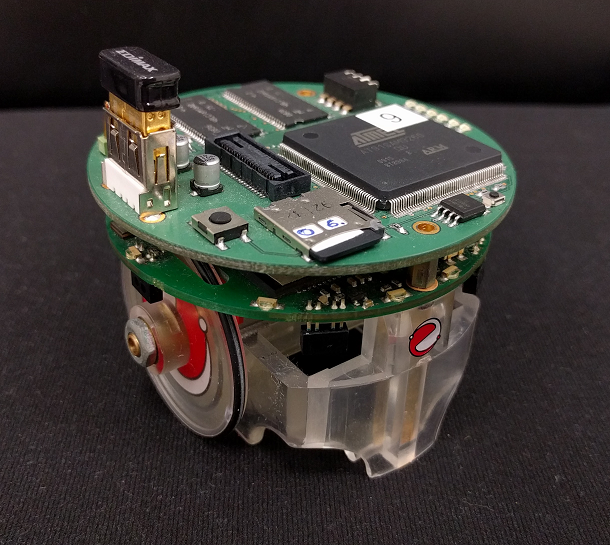
\includegraphics[scale=0.6]{EPuck.png}
	\decoRule
	\caption[The e-puck Robot]{The e-puck robot.}
	\label{fig:EPuck}
	\end{center}
\end{figure}

%----------------------------------------------------------------------------------------

\section{Processor}
The e-puck features a dsPIC 30F6014A microprocessor, designed and manufactured by Microchip Technology Inc. This is a general purpose 16-bit CPU, with relatively low performance by modern standards. The processor features 68 I/O pins, which are connected to the e-pucks various peripherals. Due to the use of the more powerful Linux extension board discussed in section \ref{LinuxExtensionBoard}, the primary use of the PIC processor in the e-puck configuration for this project is to interface with the e-puck's hardware. This involves receiving commands from the Linux extension board and sending appropriate control signals to the robot's actuators, as well as reading the robot's sensors and passing the retrieved sensor data back to the Linux extension board.

\subsection{Firmware}
Prior to the start of this project the YRL had already developed a library of low level code allowing the PIC to function in the hardware interface role as described above, controlled through the UART serial port. This firmware code was used as-is on the e-puck PIC controllers throughout the project.

%----------------------------------------------------------------------------------------

\section{Actuators}
The e-puck robot features two wheels, independently actuated by two step motors. The wheels have a diameter of approximately 41mm. The motors can rotate the wheels at an approximate maximum speed of 1000 steps per second in either direction, where 1000 steps is one full revolution. The robot also features a ring of 8 red LEDs around the edge of the main circuit board. 

%----------------------------------------------------------------------------------------

\section{Sensors}
The e-puck robot features a number of different sensor sets, of which only some are used in this project. A set of 8 IR proximity sensors are arranged around the circumference of the robot, with four positioned on the forward hemisphere, two positioned at right angles to the forward direction (one on either side) and two more positioned on the backward hemisphere at roughly 45 degrees either side of the backward direction. Figure \ref{fig:EPuckIRSensors} shows this layout. The IR sensors can be used in two modes - active and passive. In active mode the sensor emits an IR pulse and measures the IR strength of the reflection, whereas in passive mode the sensor simply samples the IR strength without emitting a pulse. The passive mode can therefore be used to get a 'background' IR reading, which can be compared to the active reading to improve accuracy. The IR sensor is of particular interest to this project as it is a frequently used tool when working with robots, especially robot swarms.

\begin{figure}
	\begin{center}
	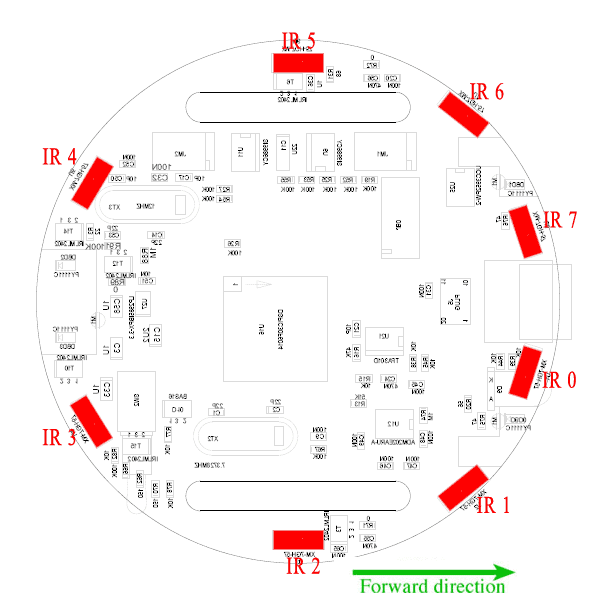
\includegraphics[scale=0.4]{EPuckIRSensors.png}
	\decoRule
	\caption[e-puck IR Sensor Layout]{The layout of the IR sensors on the e-puck robot.}
	\label{fig:EPuckIRSensors}
	\end{center}
\end{figure}

The robot also features three microphones, a 3 axis accelerometer and a camera. Due to the bandwidth required to use the microphones and camera they were considered a low priority for this project. [ACCELEROMETER?] 

%----------------------------------------------------------------------------------------

\section{Linux Extension Board} \label{LinuxExtensionBoard}
For this project the e-pucks were fitted with an extension board featuring a 32-bit ARM9 processor running a modified Linux operating system \cite{LinuxExtensionBoard}, developed by Wenguo Liu, and Alan F.T. Winfield. In this configuration the ARM processor, an Atmel AT91, takes charge of the high level robot control logic, as well as any intensive data processing operations. The dsPIC processor is then used to control the low level actuator and sensor control, running in parallel with the ARM processor and communicating via UART. The extension board provides a USB port, and for this project a WiFi adapter was connected to each robot. The controller code running on each robot could then make use of the standard IP network layer protocol, and the standard transport protocols TCP and UDP.

%----------------------------------------------------------------------------------------

% Chapter 6

\chapter[Video Tracking System]{Video Tracking System} % Main chapter title

\label{Chapter6} % For referencing the chapter elsewhere, use \ref{Chapter6} 

%----------------------------------------------------------------------------------------

\section{Overview}
In order to implement the augmented reality visualisation element of the system, and satisfy the related objectives, a live video feed of the swarm was needed. A method for tracking the positions of each individual robot in the swarm based on images from this feed was also required. Prior to the start of the project the YRL already had infrastructure in place for this kind of task, in the form of a machine vision camera placed above an 'arena', and software for processing the output of this camera using the `ARuCo\cite{Garrido:2014}' fiducial marker based tracking system. Figure \ref{fig:CameraLayout} shows the arrangement of the machine vision camera used for robot tracking, and the robot arena. It was determined that incorporating this existing infrastructure into the system was the quickest way to get this required aspect of the system working, allowing work to focus on the novel aspects sooner.

\begin{figure}
	\centering
	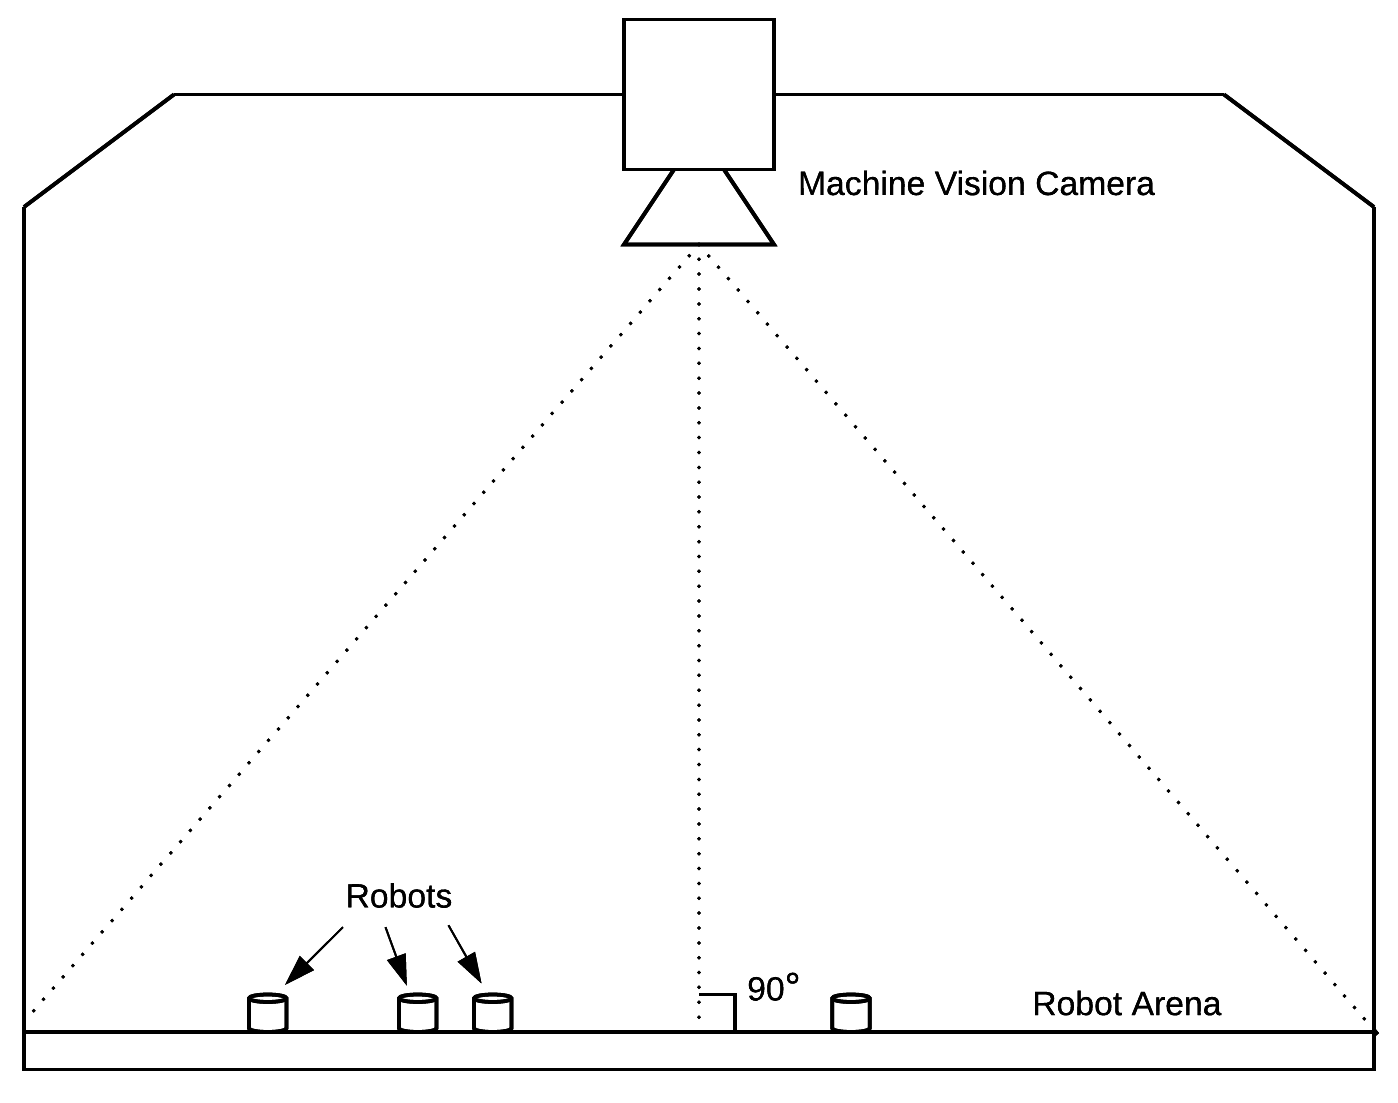
\includegraphics[scale=0.3]{Figures/CameraLayout.png}
	\decoRule
	\caption[Tracking Camera Arrangement]{Arrangement of the tracking camera over the robot arena.}
	\label{fig:CameraLayout}
\end{figure}

%----------------------------------------------------------------------------------------

\section{Camera}
[WHAT CAMERA IS USED? DETAILS.]


%----------------------------------------------------------------------------------------

\section{ARuCo Tracking System}
Developed by a team from the Computing and Numerical Analysis Department at Cordoba University in Spain, the ARuCo tag generation and detection system \cite{Garrido:2014} is a powerful fiducial marker creation and tracking tool. It comprises an algorithm for producing a `dictionary' of square, black and white, coded markers which can be printed and attached to objects and surfaces, and a method for automatically detecting these markers in a given image. The stated applications include augmented reality and robot localisation. One of the main benefits of this system over other fiducial marker systems is the execution speed. By first using edge-detection methods to find the outlines of markers in the image, the system can eliminate a large portion of the image before applying the more complex processing to identify and differentiate individual tags \cite{Garrido:2014}. This makes it possible for the ARuCo system to be run in real time, even with relatively modest computational power. In a conventional use case the orientation of the camera can be calculated based on the positions of the corners of a tag, given that the tag's orientation is known. In this use case the reverse is true, the camera's position is fixed, and therefore the orientation of the robot can be determined based on the position and orientation of the corners of its tag, relative to the camera. 

Each of the e-puck robots used in this project were assigned an ID number, and a dictionary of ARuCo tags was generated to match. The tags were affixed to the top of the robots, oriented to match their forward directions. Some cursory preliminary testing showed that the tags could be accurately and reliably detected in the camera images, at a decent frame rate. Further detail of the integration of the ARuCo marker tracking system into this application is given in section \ref{VideoFeedAndTrackingSystem}.

%----------------------------------------------------------------------------------------
% Chapter 7

\chapter[Initial User Survey]{Initial User Survey} % Main chapter title

\label{Chapter7} % For referencing the chapter elsewhere, use \ref{Chapter6} 

%----------------------------------------------------------------------------------------

\section{Overview}
In order to determine how best to implement the system in a fashion that is useful in, practice a survey was carried out at the YRL. Those asked were all actively engaged in robotics work, either in a research capacity or as a technician, and some experience and understanding of swarm robotics specifically. The survey aimed to determine first if a level on interest existed for such a system, and then which specific features were most desired. This would go on to influence design choices and inform priorities during development.

%----------------------------------------------------------------------------------------

\section{Data}
\textbf{Question 1: Do you believe that a system for displaying internal robot data for a swarm of robots in real time would be useful when debugging swarm robotics behaviours and/or conducting swarm robotics experiments?}

\begin{center}
\begin{tabular}{ c c c }
 Answer & Votes & Percentage \\ 
 \hline
 Yes & 4 & 80 \\ 
 No & 1 & 20 \\
 No Opinion & 0 & 0 \\
\end{tabular}
\end{center}

\vspace{1cm}

\textbf{Question 2: Do you believe that such a system would benefit from the inclusion of an 'augmented reality' component - whereby data retrieved from the robots could be displayed in graphical forms, overlaid on a live video feed of the robots themselves?}

\begin{center}
\begin{tabular}{ c c c }
 Answer & Votes & Percentage \\ 
 \hline
 Yes & 5 & 100 \\ 
 No & 0 & 0 \\
 No Opinion & 0 & 0 \\
\end{tabular}
\end{center}

\vspace{2cm}

\textbf{Question 3: Please rate each of the following potential features based on your opinion of their importance or usefulness to the system proposed, on a scale of one to five, where one indicates a feature is not important or useful, and five indicates a feature is very important or useful.}

On the questionnaire the values of one to five were qualified as `\textit{Not important or useful}', `\textit{Unlikely to be important or useful}', `\textit{Neutral}', `\textit{Somewhat important or useful}' and `\textit{Very important or useful}' respectively.

\begin{center}
\begin{tabular}{ p{10cm} c c c c c }
 Feature & 1 & 2 & 3 & 4 & 5 \\ 
 \hline
 Real time video feed of the robots and their environment & 0 & 0 & 0 & 0 & 5\\
 Augmentation of the video feed with the position and orientation of each robot & 0 & 0 & 1 & 1 & 3\\
 Augmentation of the video feed with each robots identifier (ID or name) & 0 & 0 & 0 & 1 & 4\\
 Augmentation of the video feed with spatially situated sensor data, represented in a graphical form & 0 & 0 & 0 & 2 & 3\\
 The ability to enable and disable individual elements of the video feed augmentation & 0 & 0 & 0 & 2 & 3\\
 The ability to customise individual elements of the video feed augmentation (colour, size, etc.) & 0 & 0 & 2 & 1 & 2\\
 Displaying the robots internal state and a history of recent state transitions & 0 & 0 & 0 & 3 & 2\\
 Displaying raw sensor data (e.g. IR) in textual format & 0 & 0 & 0 & 4 & 1\\
 Displaying sensor data in plotted graph formats & 0 & 0 & 1 & 3 & 1\\
 Support for displaying unspecified user data in textual form & 0 & 0 & 1 & 2 & 2\\
 The ability to compare two or more specific robots within the swarm & 0 & 1 & 1 & 1 & 2\\
 Logging received data and events to a text or CSV file & 0 & 0 & 0 & 1 & 4\\
\end{tabular}
\end{center}

\vspace{1cm}

\textbf{Question 4: Please briefly describe any additional features you believe would be useful, based on your experiences working with swarm robotics systems.}

\begin{itemize}
\item ``macro-level behavioural data on the swarm; e.g., number of robots in different behavioural states (color coded accordingly).''
\item ``I think the system (already potentially very useful) could be improved/expanded further to add the option of more post-processing/extraction of data. The ability to create video of the over-lay, and perform statistical analysis on the complete run, would begin to turn the system in not only a very useful debugging system but a complete package allow researchers to gather high-quality, publication ready analysis of swarm experiments.''
\end{itemize}

\textbf{Question 5: Which of the following aspects of the robot data do you believe should be made available by the application to aid in debugging and testing? Tick all that apply. Please add any more you may think of.}

\begin{center}
\begin{tabular}{ p{10cm} c }
 Data Type & Votes\\ 
 \hline
 Position & 4\\
 Orientation / direction & 4\\
 Position change over time (recent path tracking) & 4\\
 Internal state machine state & 3\\
 Internal state transition history & 3\\
 IR sensor values & 4\\
 Distance between robots & 3\\
 Robot ID & 4\\
 Other & 2\\
\end{tabular}
\end{center}

Additional responses:

\begin{itemize}
\item ``Option to include user-defined data so if a certain controller implements a timer that facilitates a state transition might be useful to see the value of that timer whilst debugging to compare with state transitions''
\item ``A simple API to add user-defined variables/statuses''
\end{itemize}

\textbf{Please add any additional comments you have about the proposed application in relation to your experiences working with swarm robotics systems.}

\begin{itemize}
\item ``A client-server model between back-end (camera) and remote client would potentially be very useful; also the system should be flexible and not reliant on a specific camera/server setup. Would be very interesting to see if it will work on a R-Pi 3 + camera combination, as this would allow for portable tracking setups.''
\item ``All real-time information is useful!''
\end{itemize}

%----------------------------------------------------------------------------------------

\section{Analysis}
The positive response to question one indicates a reasonable level of interest in the system amongst those surveyed. The similarly positive response to question two adds more weight to the idea that graphical debugging tools have the potential to be particularly useful in a robotics context, as established during the literature review. The responses to these two questions indicate that interest exists for the system, and that it is worthwhile implementing it. This satisfies the first aim of the survey.

The remainder of the survey focuses on establishing which features are most desirable, and the results were used when considering implementation priorities. The response to question three indicates that the majority of the core features were thought to be potentially useful, especially those related to the video feed and overlay. Tertiary features such as customising the colours and sizes of the overlays showed less interest. This was as expected, as these kinds of features do not aid directly in the debugging process. Considerable interest was expressed in the ability to log data and events, a feature which was not considered a major priority at the outset. Conversely, the ability to compare two robots was the only feature to receive a vote lower than neutral, despite being initially thought a key feature of the system. As a result the implementation of logging was moved up to a main priority, and the comparison feature was reduced to non-essential.

The respondents were then given the chance to optionally suggest additional features in question four. The first of the two responses suggests `macro-level behavioural data', a concept considered during the project's inception. It was not included in the initial plan or survey partly because at the outset it was not clear what form the feature would take, or whether it would be feasible in the time frame, and partly because it was seen as a feature related more to analysing swarm experiments and results rather than debugging. As a result of this answer displaying macro level swarm data was considered a desirable but not essential feature, to be implemented if time allowed. The second response offers a broader vision for the system as a whole. This report agrees with the observation of the systems potentially to become a complete package for analysing swarm experiments and extracting data, however the majority of the features mentioned are considered beyond the scope of this project. This includes video extraction and post processing of data. These are however considered in section [??] regarding future work, as they present significant potential expansions of the system.

Question five attempts to establish which specific data types are most desirable in the system. Note that one respondent did not answer this question at all, leading to the lower vote counts. None of the data elements listed received a significant deficit in votes, suggesting that all the data types listed should be included. Respondents were asked to optionally suggest other data types, and the two responses received both independently identified user-defined data or 'variables' as a desirable data  type. The inclusion of custom user defined data was a planned part of the system from the beginning, and is mentioned in question 3, but these responses confirmed that it should be a priority feature of the system.

The final section gave respondents the opportunity to add any additional comments about the system. The first response notes that designing the system in a way which does not make it `reliant on a specific camera/server setup' would improve its usability. This thinking matches the stated objective of making the system in a modular way that is easily extensible with different camera set-ups and different robots.

%----------------------------------------------------------------------------------------

\section{Issues and Shortcomings}
This survey provided a useful tool for gathering a general impression of relevant opinions regarding the project and the system. However it also had a number of issues in its execution which might somewhat diminish the value of the data. Firstly due to the highly specific nature of the desired participants, the sample size is extremely small. Care must therefore be taken in analysing too deeply the results; for example any statistical analysis performed would likely be flawed. Another issue is that the two larger multiple choice questions present a relatively small selection of possible features and data types, based on those already planned or considered for implementation.  This report therefore aims to use the results in an indicative, holistic manner to guide implementation, rather than quantitatively define the feature set.

%----------------------------------------------------------------------------------------

% Chapter 8

\chapter[Design]{Design} % Main chapter title

\label{Chapter8} % For referencing the chapter elsewhere, use \ref{Chapter8} 

%----------------------------------------------------------------------------------------

This section describes the design of the system, and gives details of the reasoning behind some of the design decisions. This design work was done largely prior to implementation, with some elements of the design being re-factored during the implementation phase in adherence to the agile development methodology being followed. The design process was separated into a number of key areas. Firstly a software architecture design was produced, including a breakdown of the system in terms of individual components and a description of the intended path of data through the system. This served as a road map during the implementation stage. The second key area was the user interface design. This involved determining how the main application should appear to the user, and how best to provide the user with access to the various features, and then creating a template of the window and component layout required to achieve this. The graphical representations for each of the data types to be displayed in the visualiser were also designed.

%----------------------------------------------------------------------------------------

\section{Software Architecture Design} \label{SoftwareArchitectureDesign}
The guiding principles of the software architecture design were `Object Oriented Programming' (OOP) practices, and the `model-view-controller' (MVC) software architecture pattern. OOP \cite{OOP} is an extremely widespread concept in modern software development theory. It states that code should be organised into units based on individual functionalities, commonly referred to as classes. Each class collects together the data that describes an object and the routines to perform actions with and on that data. A class then acts as a template, and a new instance of the class can be instantiated each time an object of that type is needed. OOP aims to make code easier to understand and maintain, reduce code duplication, and increase re-usability and modularity. Designing software in an OOP fashion is standard practice for most modern programming tasks, and modern languages are often designed around OOP concepts.

C++ was selected as the development language for this application as it offers much of the low level control and efficiency of the C language, whilst also supporting OOP practices natively. The majority of the existing software infrastructure in the YRL had also been implemented in C++, hence following suit would help with maintainability and integration in the future. Considering the project's requirements for interfacing with low level hardware such as the tracking camera (via a driver) and the robots (via network sockets), and for performing image processing, the speed and low level capabilities of C++ also seemed beneficial. Higher level languages such as Java were considered, as they offered a number of different benefits such as better portability and automatic resource management, but were ultimately deemed less suitable.

The MVC \cite{MVC} software architecture design pattern is another widespread concept in software development theory. It primarily relates to the programming of application user interfaces. The three words that give the pattern its name - model, view and controller - define the three 'layers' into which code components are organised. The model refers to the application's data, and includes all of the information that defines the application's current state. The view refers to the code used to produce the user interface from the data in the model layer. It acts as the method by which the user 'views' the data. Finally the controller layer acts as the intermediary between the two, retrieving data from the model and processing it if necessary before passing it to the view for display. The controller also responds to inputs, and modifies the data in the model accordingly. This includes user input, as well as input from other sources. In the case of this application these other sources include the tracking camera and the robots, which send their input via the Ethernet cable and WiFi network respectively. 

The MVC pattern specifies that all components must exist in one of these layers, and the layers must be kept separate. Adhering to an MVC pattern ensures that state data is not maintained or duplicated within the UI code, and that only one, true copy of the application data exists, stored in the model layer. Separating the functionalities in this way also helps to keep code structured and organised, making it easier to understand, maintain and extend, as changes to the internals of a component in one of the layers should not affect components in the other layers.

With these two principles in mind, the software design process could begin. First the application was broken down into individual components based on the functional specification. The following key components were identified:

\begin{itemize}
\item Code to handle communicating with the camera and retrieving the image data.
\item Code to perform the robot tracking.
\item Code to handle the networking, including receiving data from the robots.
\item Code defining a model to store the robot data in.
\item Code to enter new data into the model.
\item Code to augment the video feed based on the stored data.
\item Code to display the video and augmentations feed to the user.
\item Code to respond to user input via the user interface.
\item Code to store settings related to the application.
\end{itemize}

\begin{figure}[h]
	\centering
	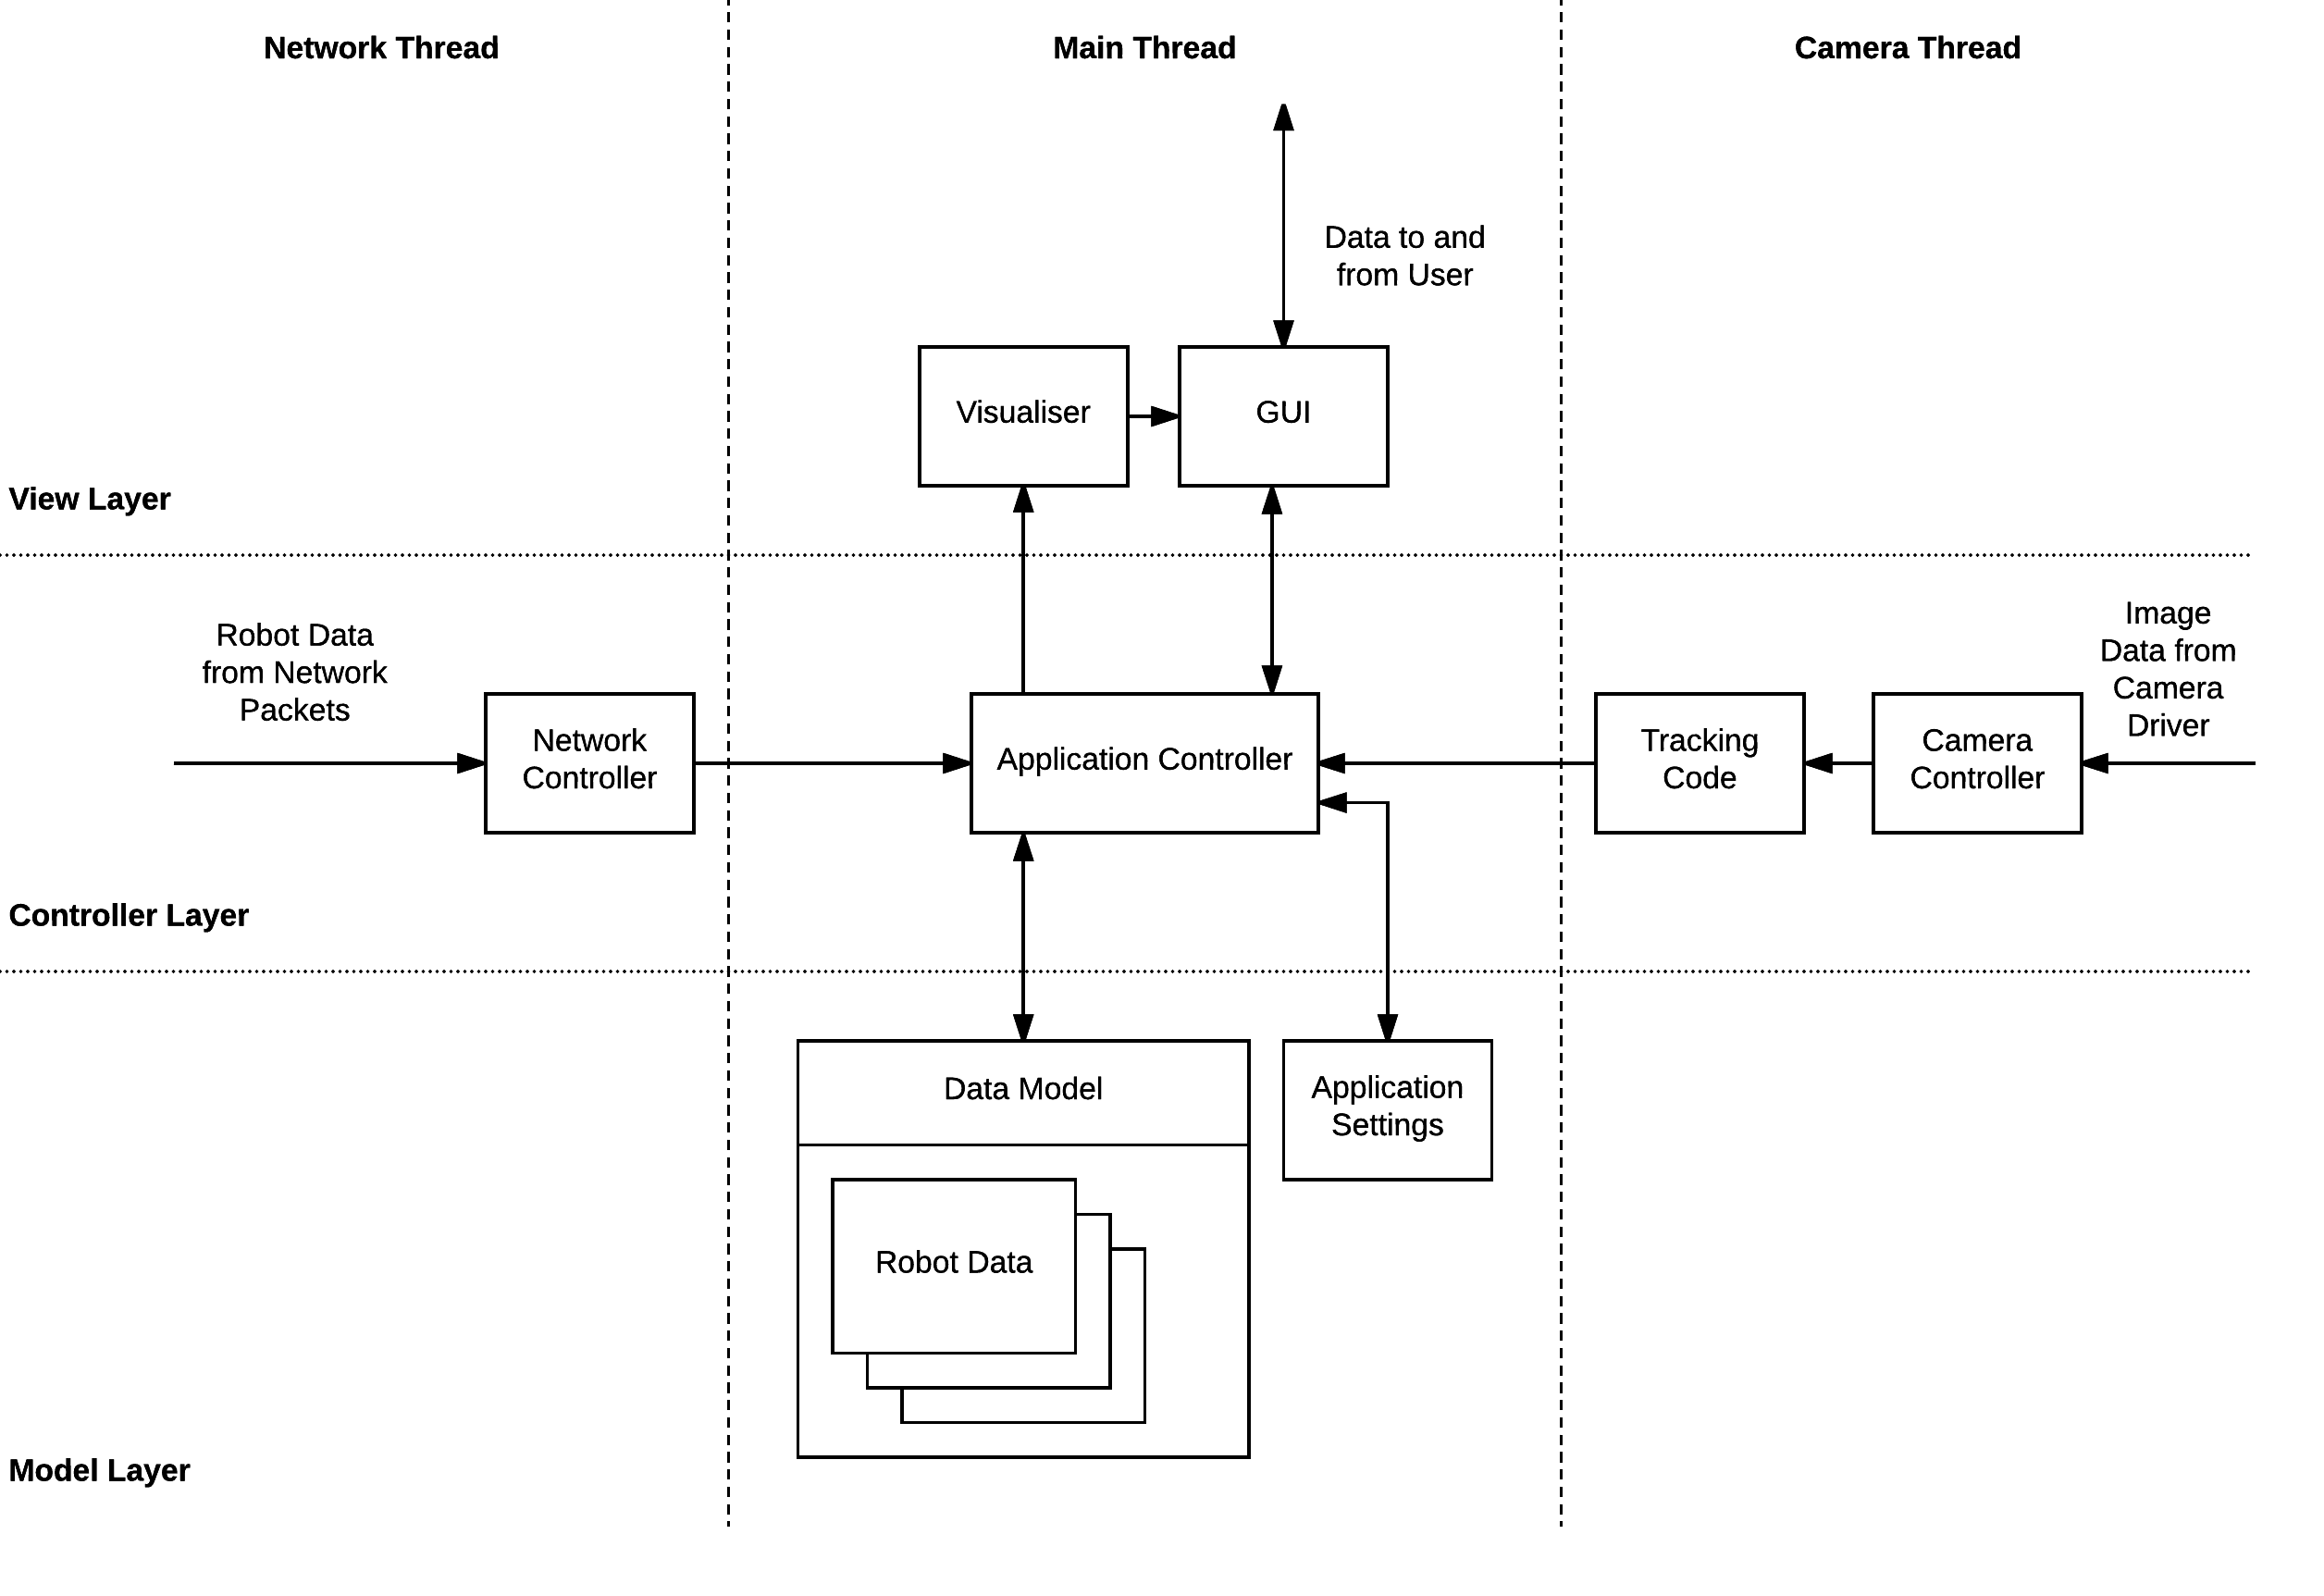
\includegraphics[scale=0.7]{Figures/SoftwareArchitecture.png}
	\decoRule
	\caption[Software Architecture Diagram]{A diagram of the software architecture design and data flow.}
	\label{fig:SoftwareArchitecture}
\end{figure}

Once separated into functional components, the required code blocks could be organised into a structure, and the data path of the application examined. Figure \ref{fig:SoftwareArchitecture} shows this structural arrangement, with boxes for each of the functional objects and arrows indicating data flow. The three layers of the MVC design pattern are shown by the vertical partitioning. The horizontal partitioning is used to show another key design consideration - threading. In order to maximise performance and ensure responsiveness, functionality which has the potential to `block' execution whilst waiting for a result or response should be run in a separate thread. This application was therefore designed with three threads in mind. The main thread handles the core of the application, including all data model access and GUI operations. The network thread handles communicating with the robots via WiFi. It was anticipated that this networking would involve low level socket code, which meant the potential for blocking socket-read operations, therefore requiring a separate thread. The camera thread handles reading the machine vision camera and performing the tag tracking using the ArUco library. It was anticipated that the camera read operation could block until the next frame was available in the camera driver's buffer. Tracking the robots in the image using the ArUco library also had the potential to be CPU intensive, so keeping this off the main thread was considered a potential performance benefit.

As can be seen in figure \ref{fig:SoftwareArchitecture}, the software architecture is structured around a central application controller. The data from all other components of the application flows through this central component, which routes it to where it needs to go. It is also responsible for updating the visualiser and GUI with new data when necessary, and acting on the user input signals received through the UI. The other key controller layer components - the network controller and the camera controller - exhibit data flow in only one direction. The design of these components was therefore relatively simple, as they needed only to perform the following loop of tasks:

\begin{enumerate}
 \item Receive data from external source.
 \item Process data as necessary, extracting required information.
 \item Notify the application controller of the newly available data.
 \item Wait for new data to become available. Return to step 1.
\end{enumerate}

The remaining components are more complex, and required greater software design considerations. The design of the data model is discussed in section \ref{DataModelDesign}. The design of the visualiser code is discussed in section \ref{VisualiserDesign}.

\subsection{Data Model} \label{DataModelDesign}
\begin{figure}[h]
	\centering
	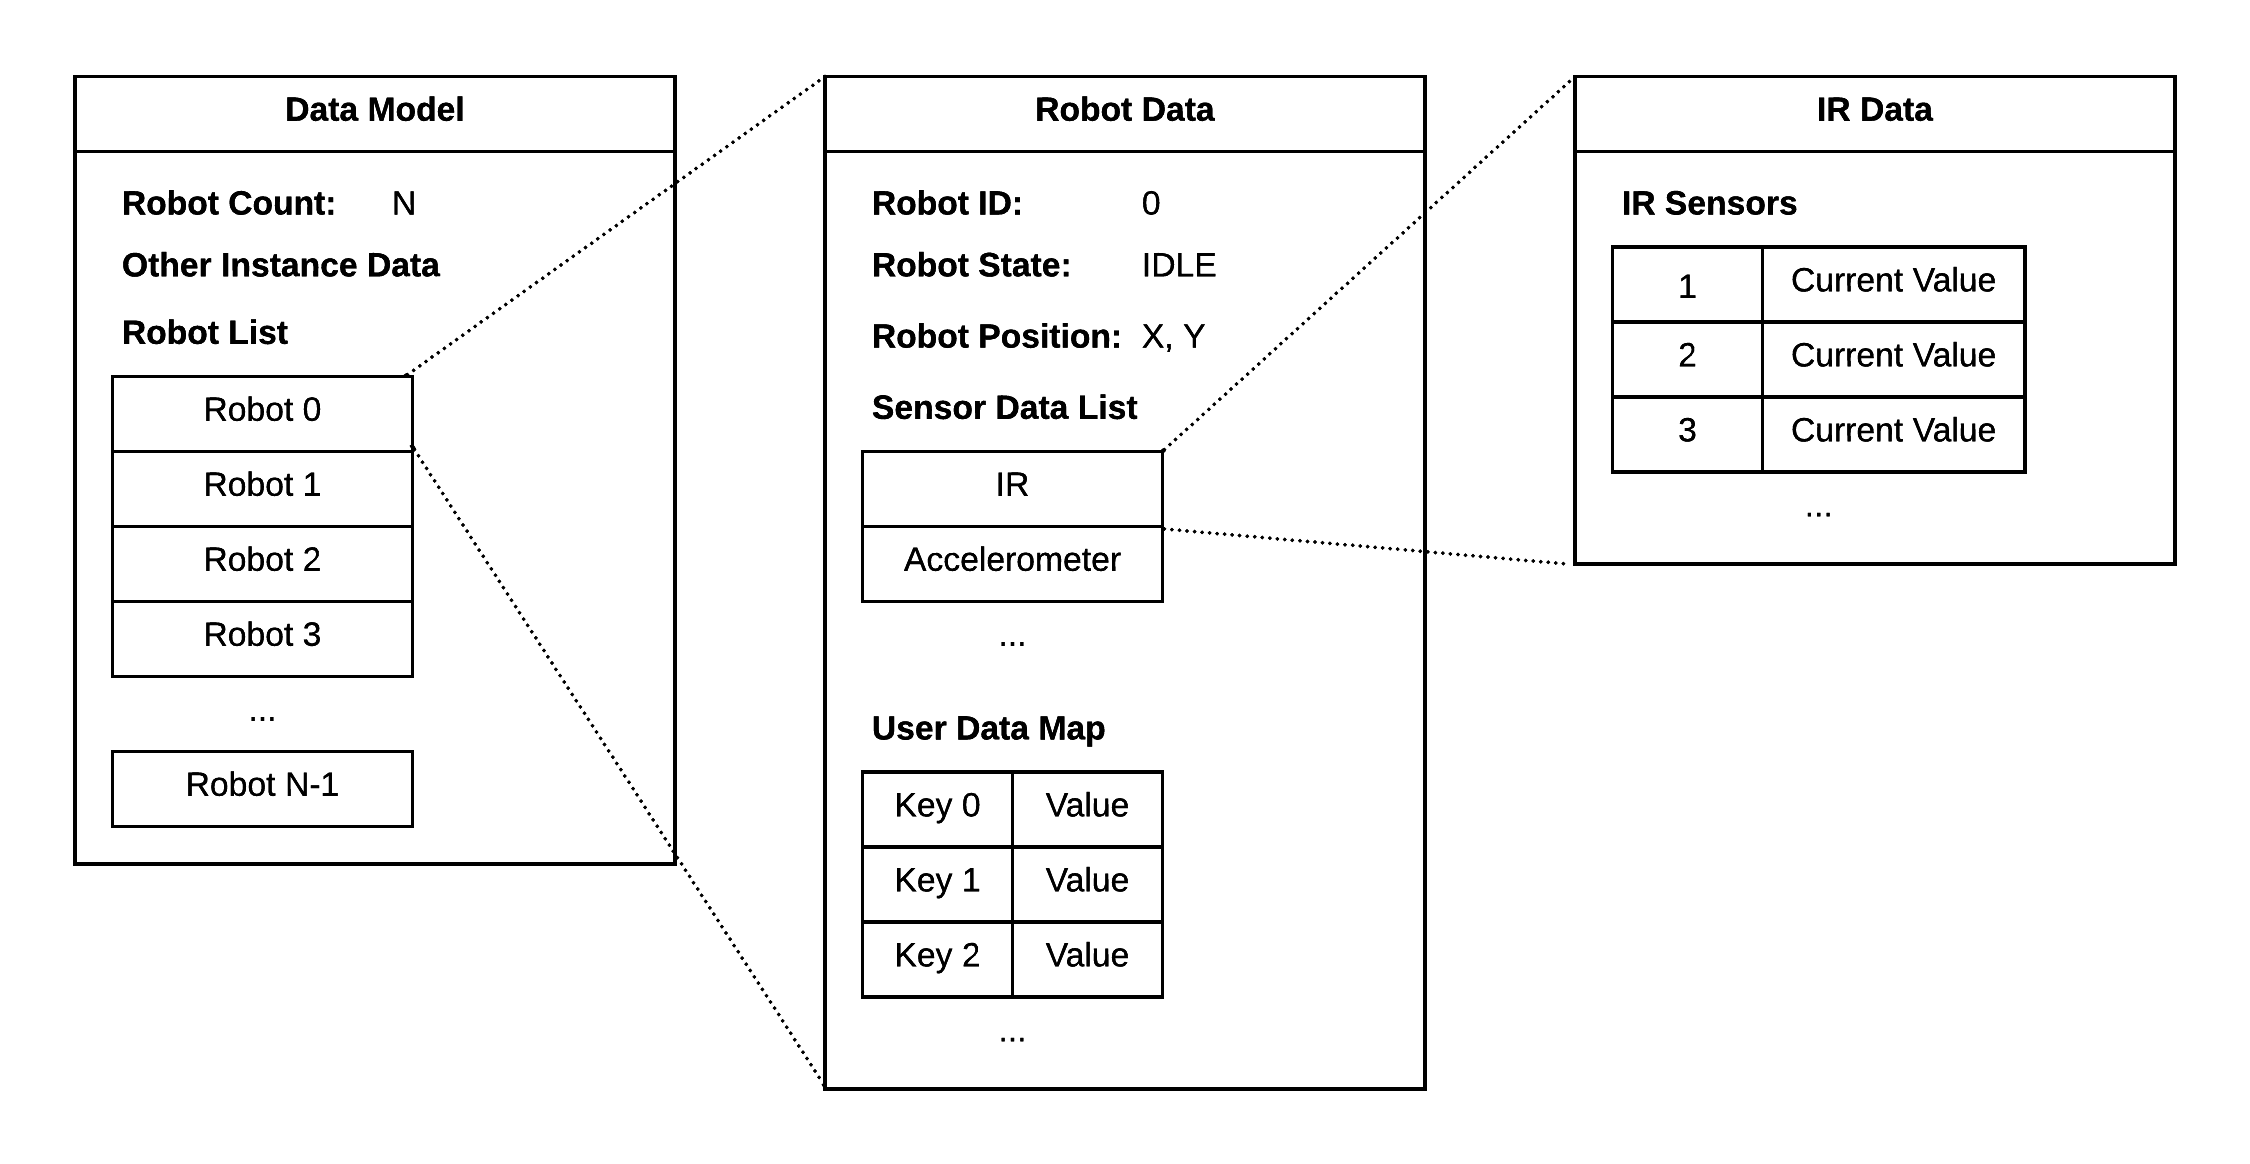
\includegraphics[scale=0.7]{Figures/DataModel.png}
	\decoRule
	\caption[Data Model Diagram]{A diagram of the data model design.}
	\label{fig:DataModel}
\end{figure}

The purpose of the data model component is to store all of the data required to describe the application's current state. This includes all data related to each of the robots being tracked by the system. In order to achieve this in an object oriented manner the data model itself was designed to comprise a number of smaller components in a hierarchical structure. The main data model object maintains a collection of smaller objects, each containing the data related to a single robot. These in turn maintain a collection of different data objects relating to the robot's state and sensor data. Figure \ref{fig:DataModel} illustrates this hierarchical data model design using the IR sensor data of a single robot as an example.

This follows object oriented programming practices by defining a single class to describe a robot, from which a new robot data object can be instantiated each time the system begins tracking a new robot. When data is received regarding a robot the system is already aware of, it can simply update the correct existing robot data object with the new data.

\subsection{Visualiser} \label{VisualiserDesign}
\begin{figure}[h]
	\centering
	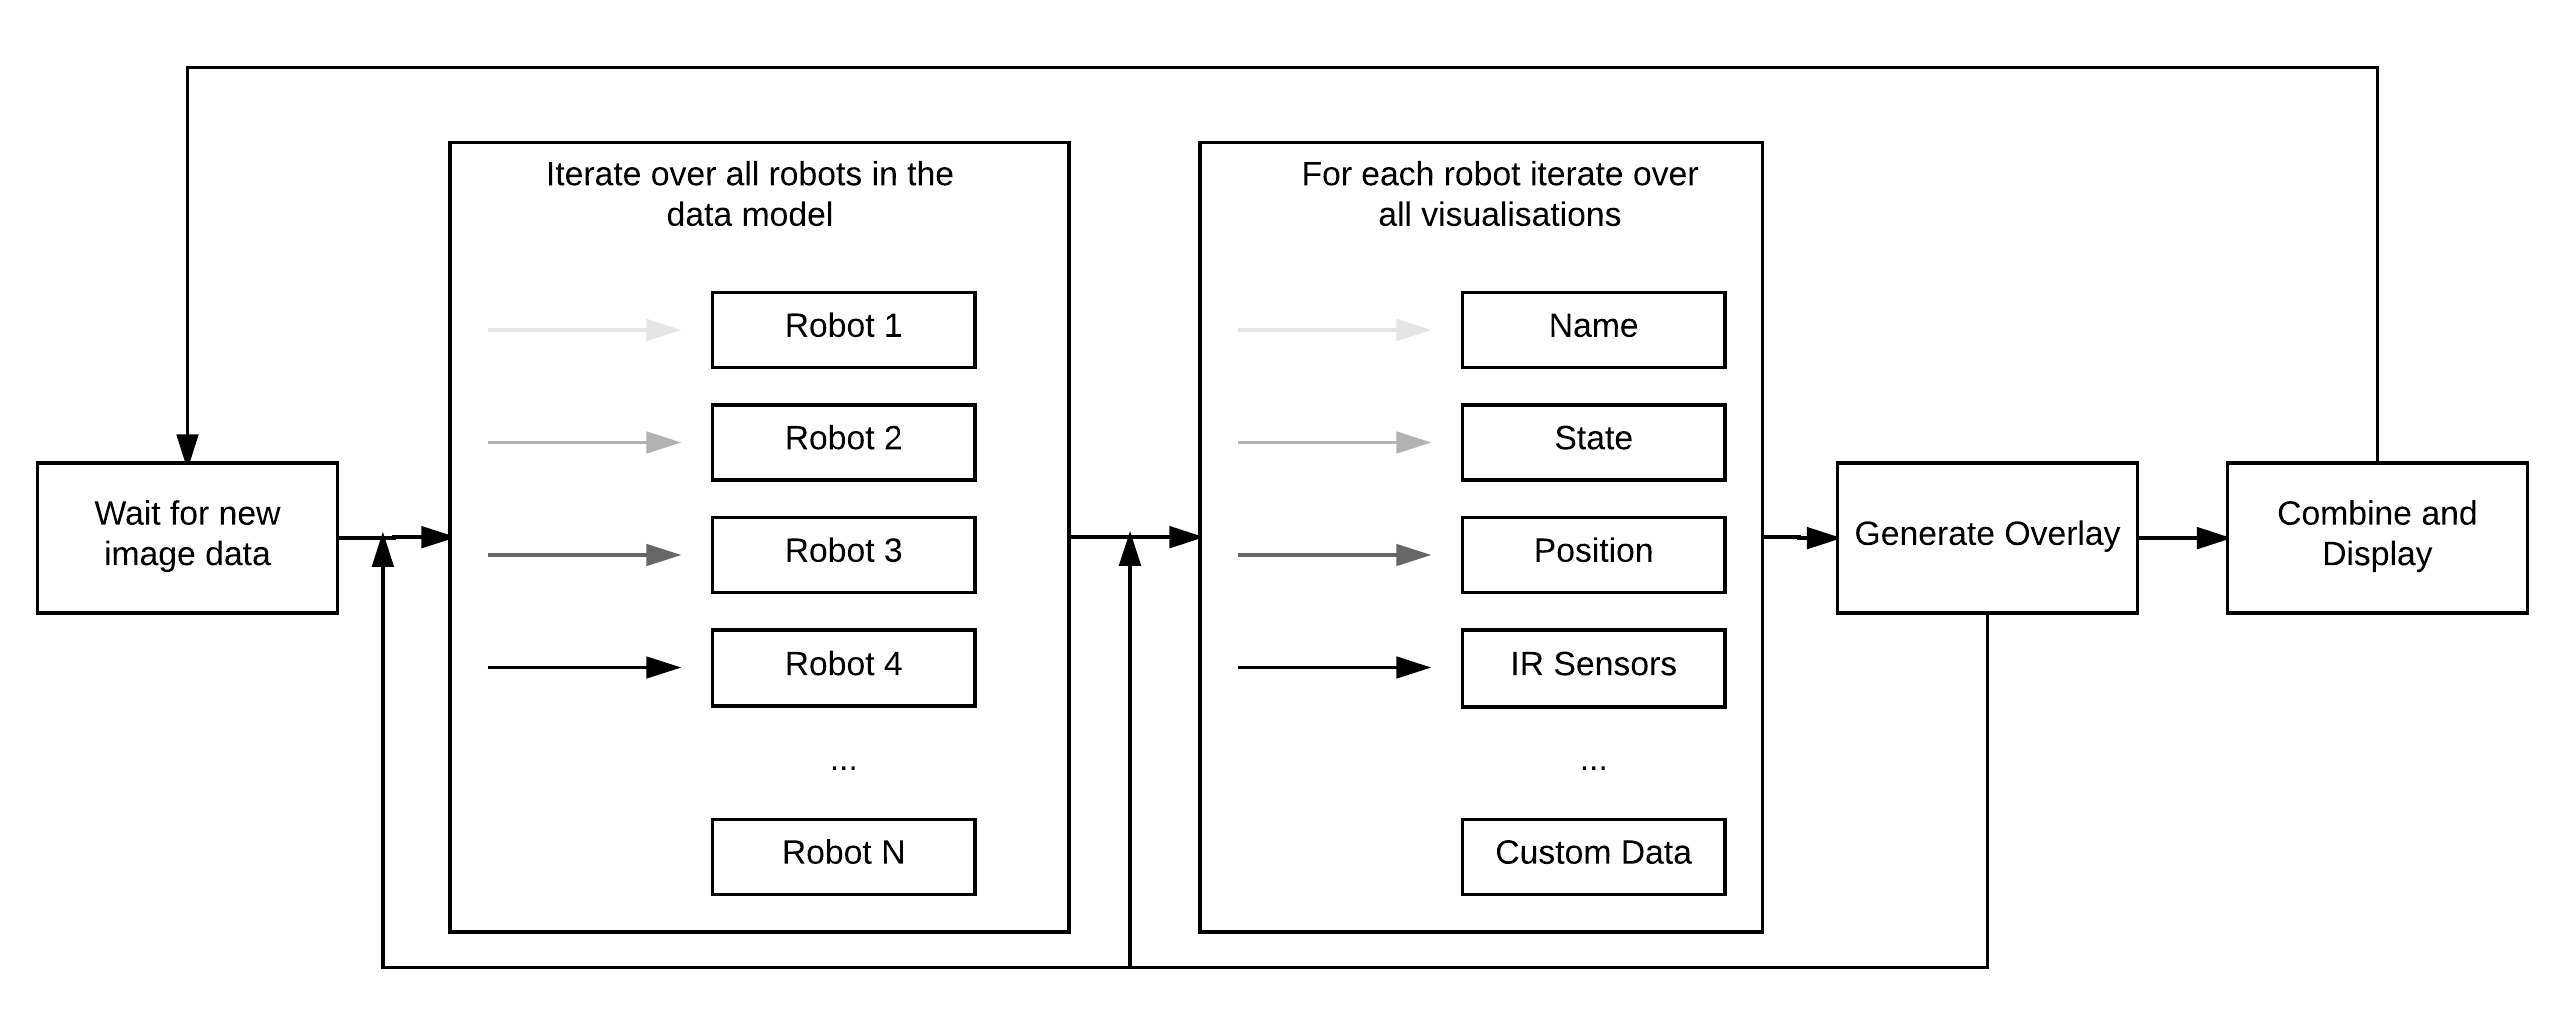
\includegraphics[scale=0.7]{Figures/VisualiserProcess.png}
	\decoRule
	\caption[Visualiser Render Process Design]{A diagram describing the design of the visualiser rendering process.}
	\label{fig:VisualiserProcess}
\end{figure}

The purpose of the visualiser component is to generate and display the augmented video feed to the user. The component must receive the latest camera image and the most up to date robot data, and generate the graphical overlays based on a combination of the robot data and the current settings for each visualisation. It can then display the latest image, with the graphical overlays applied, to the user by rendering it as a single image within the appropriate GUI element. This rendering process must occur each time a new video frame is read from the camera, hence both the video and the overlays should update regularly and respond rapidly to changes in the robot data.

In order to further modularise the visualiser code, it was broken down into a number of smaller components. For each type of data visualisation a separate component was defined, which describes how the visualisation for that data type is generated, based on a single robot data object. The main visualiser component could then be designed to generate the graphical overlays iteratively, by stepping through the available set of robot data objects, and for each one stepping through the different visualisation components, generating an overlay for each combination. The overlays can then be combined and displayed as a single image. Figure \ref{fig:VisualiserProcess} describes this process diagrammatically.

%----------------------------------------------------------------------------------------

\section{User Interface Design} \label{UserInterfaceDesign}
\begin{figure}[h]
	\centering
	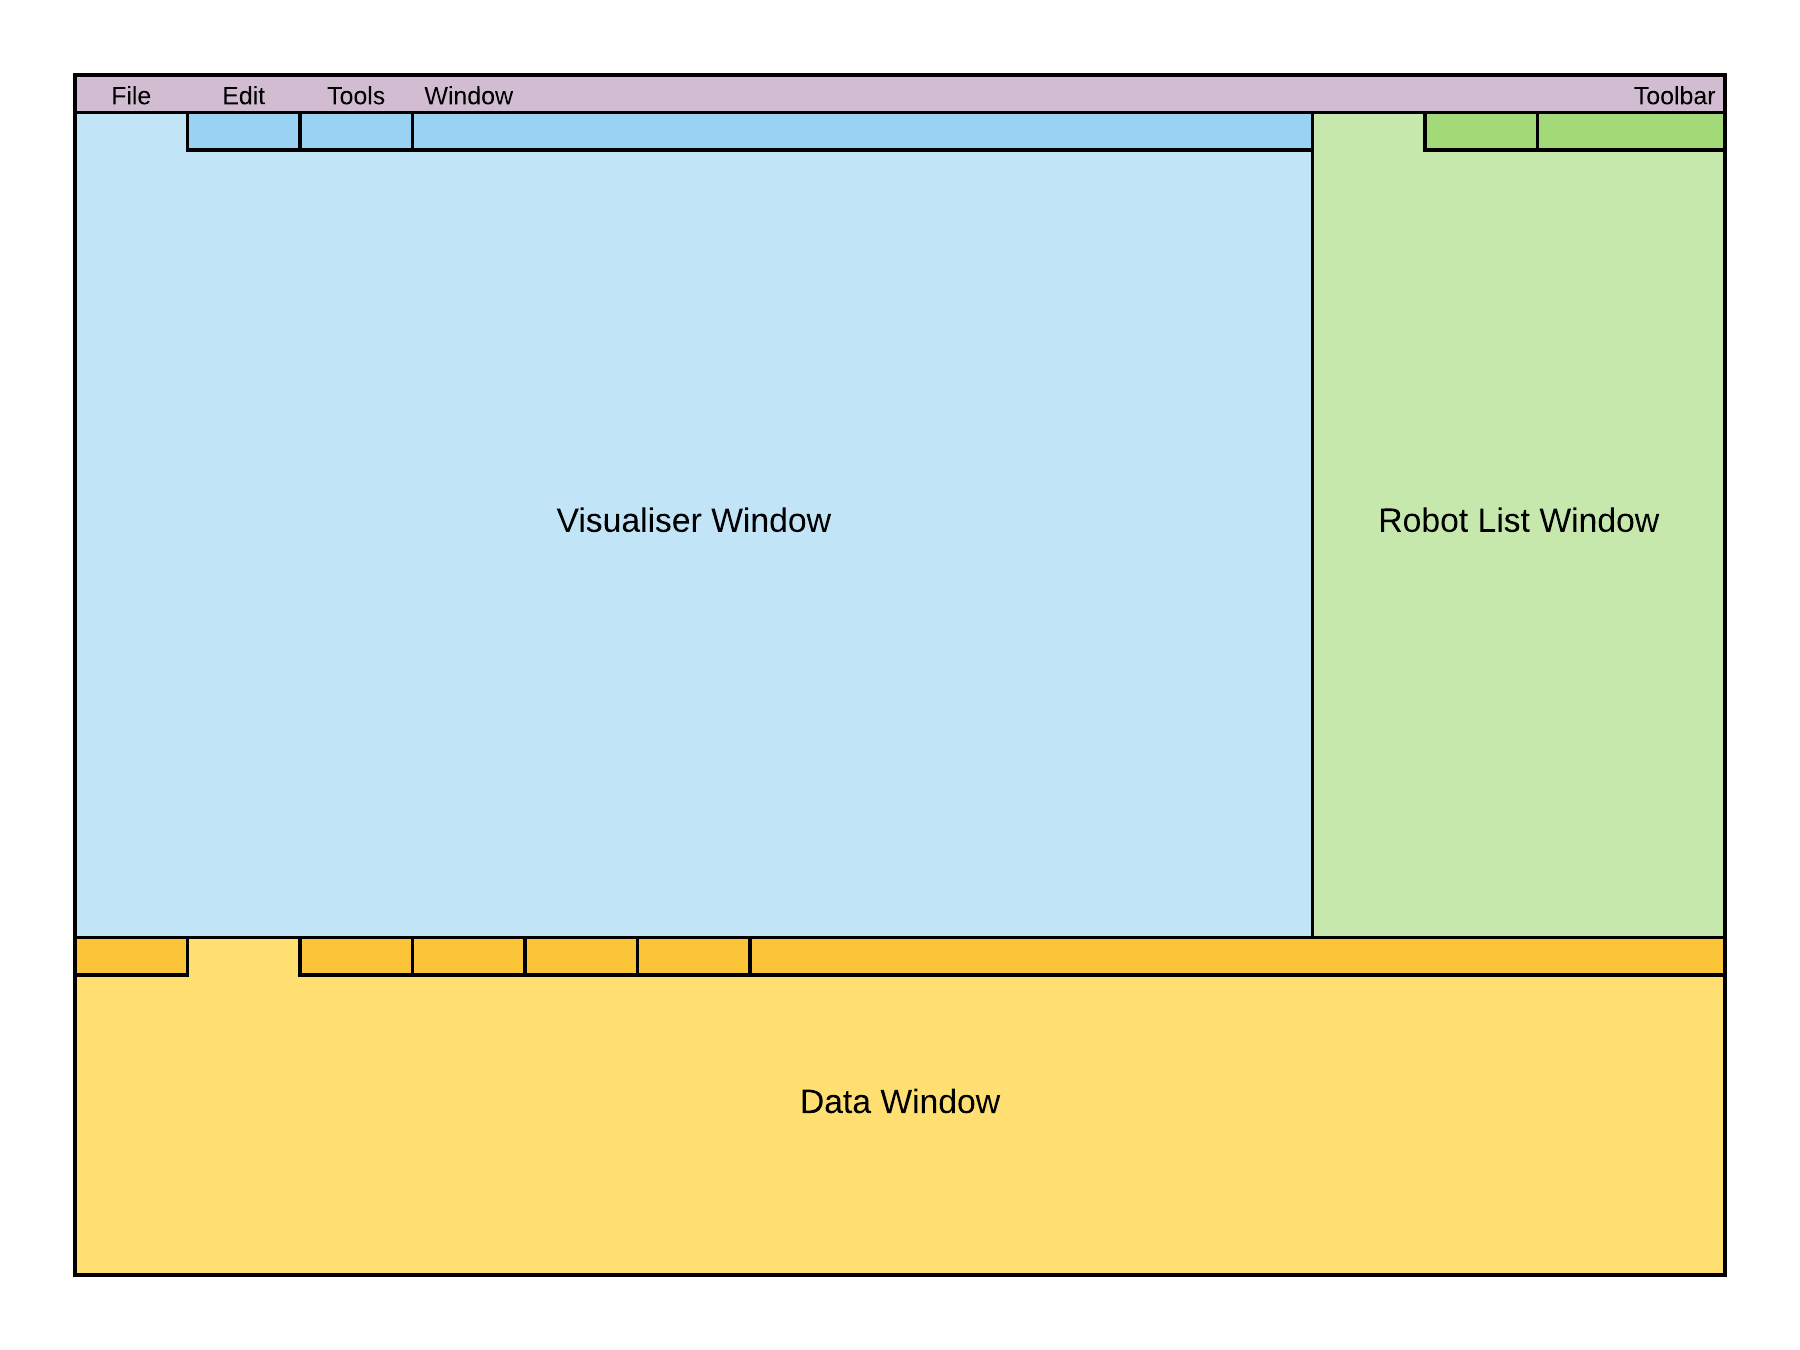
\includegraphics[scale=1]{Figures/UILayout.png}
	\decoRule
	\caption[UI Layout]{The design of the basic user interface layout.}
	\label{fig:UILayout}
\end{figure}

The second main area of consideration during the design phase was the Graphical User Interface (GUI). It was determined that creating a well-designed, intuitive interface would be essential to satisfying the objective of providing data in a 'human readable' form. Having real time data would be useless if the user cannot parse the data displayed sufficiently quickly, due to a poorly designed or confusing UI. The first decision made was to try and keep the interface familiar to a computer user, through the use of standard, widely understood user interface elements. 

There exists a well-defined `language' in computer interface design, using constructs such as windows, panels, tabs, buttons, text fields and other elements which have well-understood functions. It was thought that basing the user interface design on this well-established standard would minimise the time for a new user to become accustomed to the system. The next step was determining how many panels would be necessary for the intended functionality to be possible, and how best to lay these out within the window and organise the smaller elements within each panel. Three main panels were determined to be necessary. The first would display the video feed and visual overlay, the key component of the application. A second panel would be used to display a list of the robots known to the system, so that they could be selected without obscuring the video feed. Finally a third panel would be used to display more detailed information about the selected robot in a number of different tabs. Figure \ref{fig:UILayout} shows the basic layout design for these main panels.

The visualiser panel, highlighted in blue, takes primary place in the layout. In order to maximise the size, and therefore the readability, of the augmented video feed it was determined that this panel should occupy as much space as possible. A number of tabs allow the user to change the focus of the panel, giving access to various settings, including settings for the visualiser and camera. The robot list panel is highlighted in green on the right hand side. This requires less width, as its main function is to display a list of the known robots, and allow the user to select one. Again tabs within the panel allow the user to access functionality related to the robots, such as settings for the network connection. Finally the data panel is highlighted in yellow at the bottom of the layout. Each of the tabs provide more detailed information on a specific type of data collected about the selected robot, as well as a tab for a general overview, and a console-style log of application events. It was noted that when displaying data in this panel it should be formatted to maximise the use of the available space. This means using the full width of the window and limiting the height to avoid excessive scrolling. The design also includes a toolbar at the top of the window, another standard feature of window-based software applications. The toolbar is provided to allow quick access to useful functionalities.

\begin{figure}[h]
	\centering
	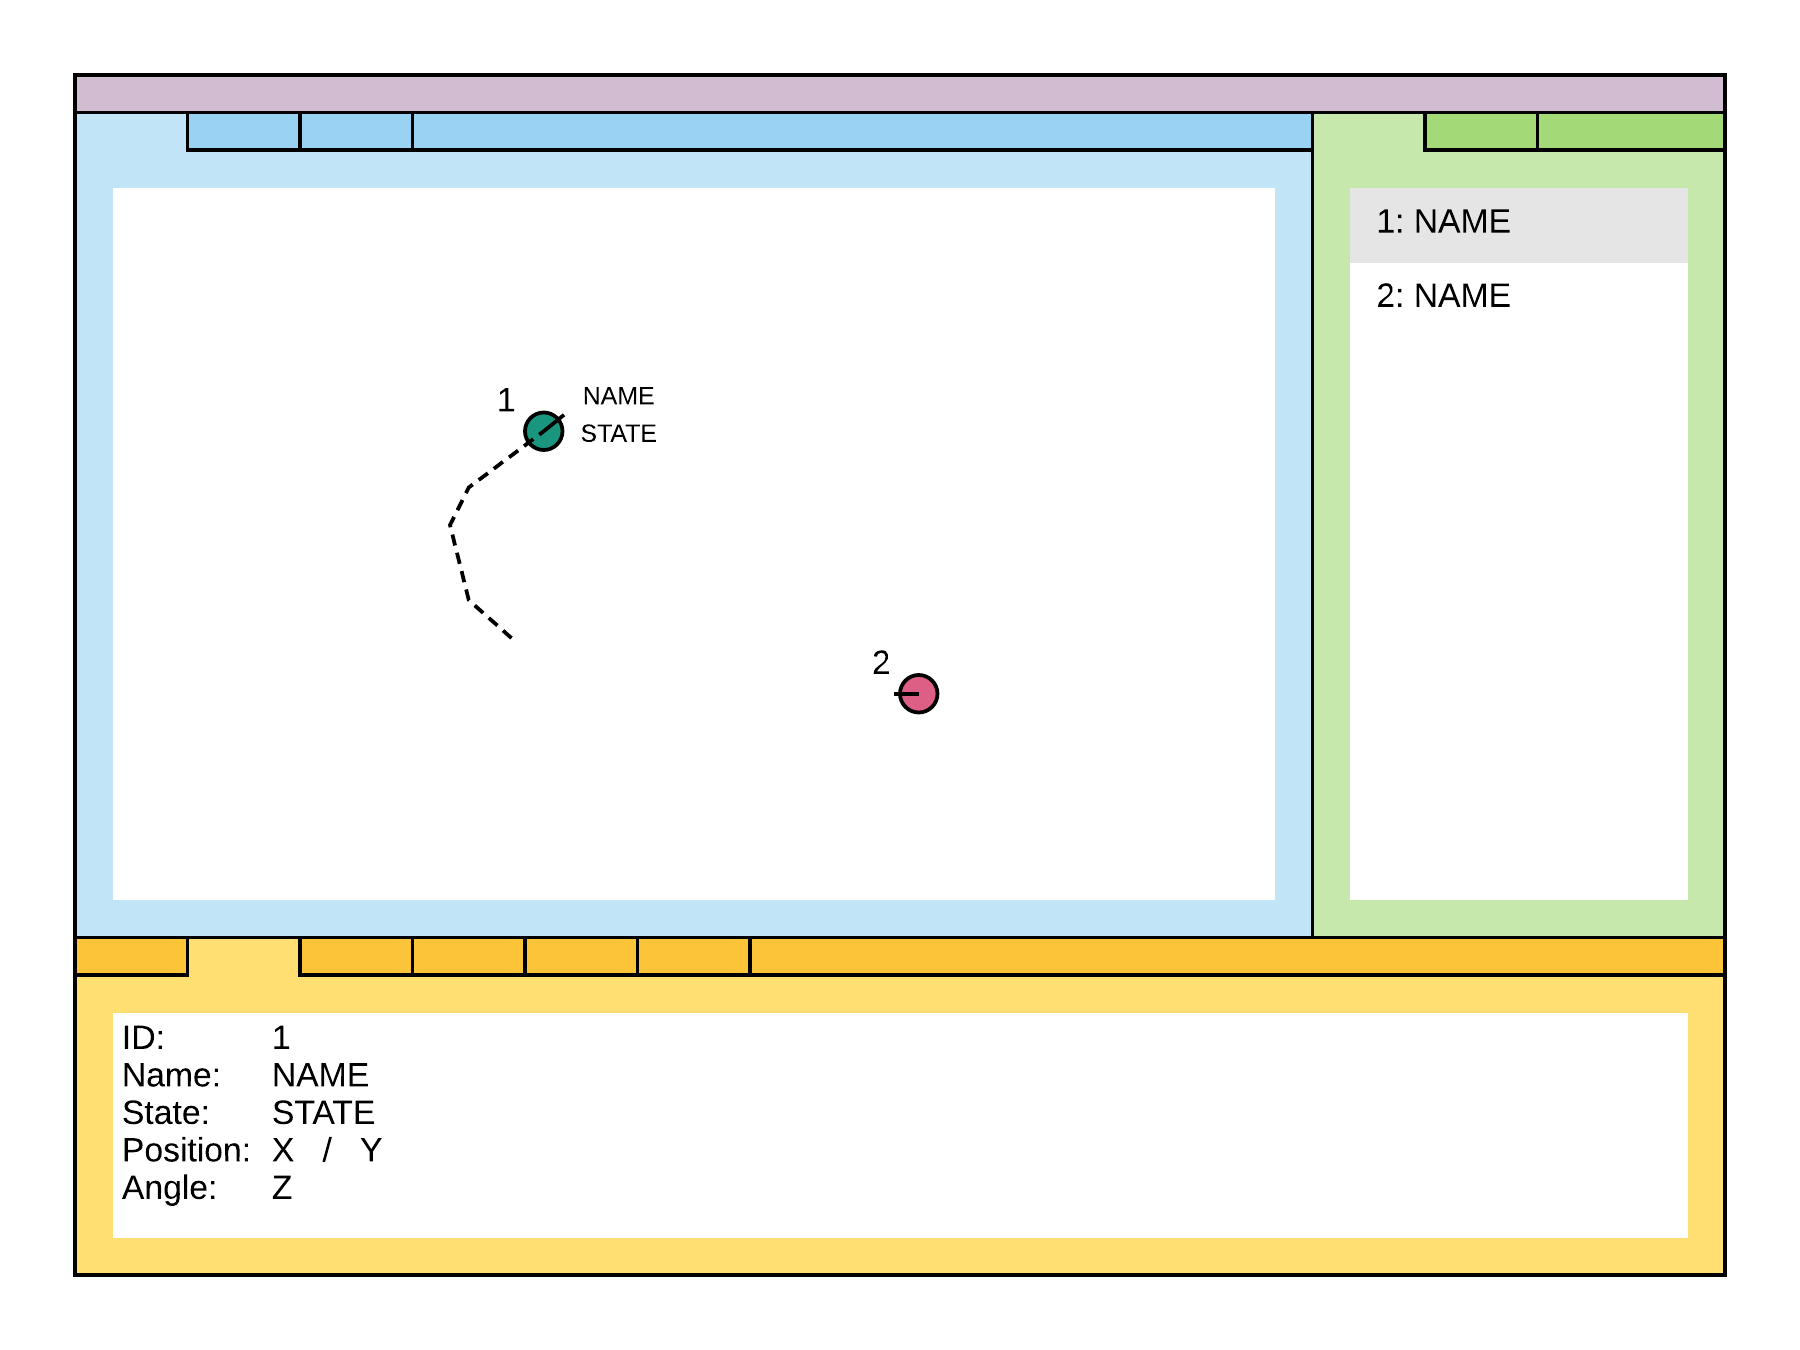
\includegraphics[scale=1]{Figures/UIExample.png}
	\decoRule
	\caption[UI Example]{The basic UI design, filled with some example content.}
	\label{fig:UIExample}
\end{figure}

Figure \ref{fig:UIExample} shows how this layout might look when filled with some example content. The robot list identifies the two robots being tracked by the system, and shows that robot 1 is selected. The visualiser component shows an example of how the video image might be augmented with graphical overlays generated from data regarding the two robots. These overlays include indicators for each robot's position and orientation, as well as text showing the name and state of the selected robot. The dotted line shows the recent path taken by the robot, which is an example of one potential type of data visualisation. Colour is also used to differentiate the two robots. The data view at the bottom of the window shows some example data for the selected robot, which might be seen on a general `overview' tab.

Time was also spent creating more detailed designs for some of the individual tabs within the main panels. Each tab within the data panel needed to display a different data type, and therefore required a unique layout and design. Figure \ref{fig:DataPanelDesigns} shows the initial designs for four of the key tabs, using both textual and graphical approaches to data representation. Layout 1 shows the overview tab design, as seen previously. Layout 2 shows the design for the console tab, which displays messages about the application sequentially. Layout 3 shows the state tab, which offers additional information about the state of the selected robot, beyond simply its current state. The first box displays a list of all of the robot's known states, and the second box displays a list of the robot's recent state transitions, including the original state, the new state and the time the transition occurred. Finally layout 4 shows one possible design for displaying the robot's IR sensor data, using a bar graph to give a relative, comparable impression of each sensor's value, and the numerical displays beneath to provide the actual sensor values. 

Figure \ref{fig:VisualiserSettingsTabDesign} shows the design for the settings tab of the visualiser panel. The purpose of this tab is to provide access to general settings related to the visualiser, and specific settings for each of the data visualisation types. The actual settings shown in the design are representative. General settings are changed using basic form controls such as tick boxes. Settings for specific visualisations can be changed using extra pop-up windows accessed by double clicking the relevant visualisation in the list. In figure \ref{fig:VisualiserSettingsTabDesign} the IR data visualisation settings are shown as an example.

\begin{figure}
	\centering
	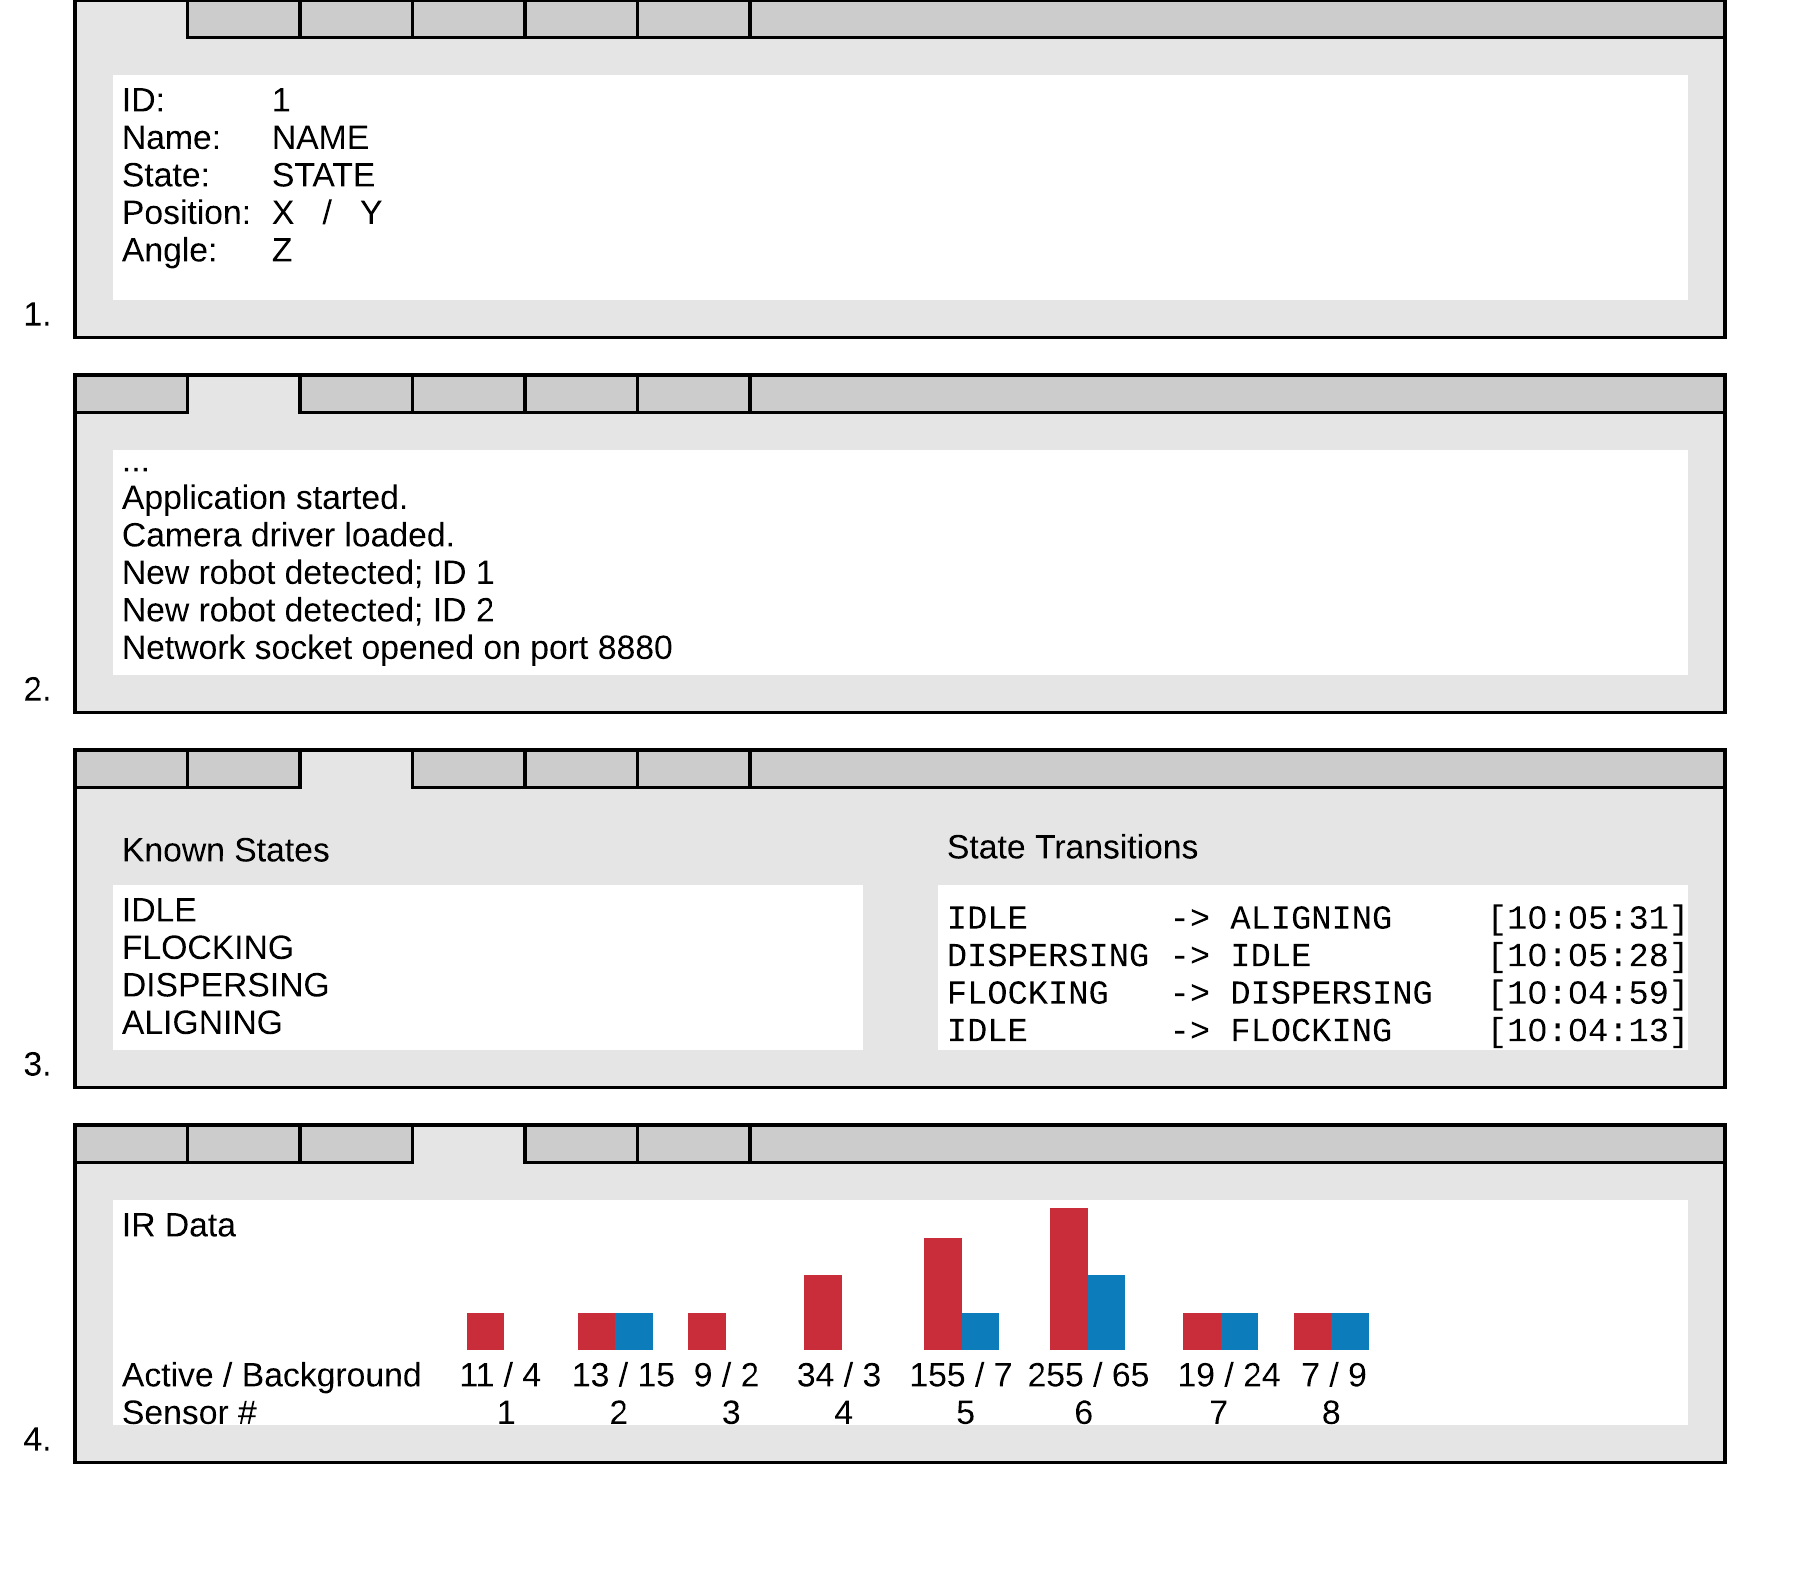
\includegraphics[scale=1]{Figures/DataPanelDesigns.png}
	\decoRule
	\caption[Data Panel Designs]{The initial UI designs created for some of the tabs within the data panel.}
	\label{fig:DataPanelDesigns}
\end{figure}

\begin{figure}
	\centering
	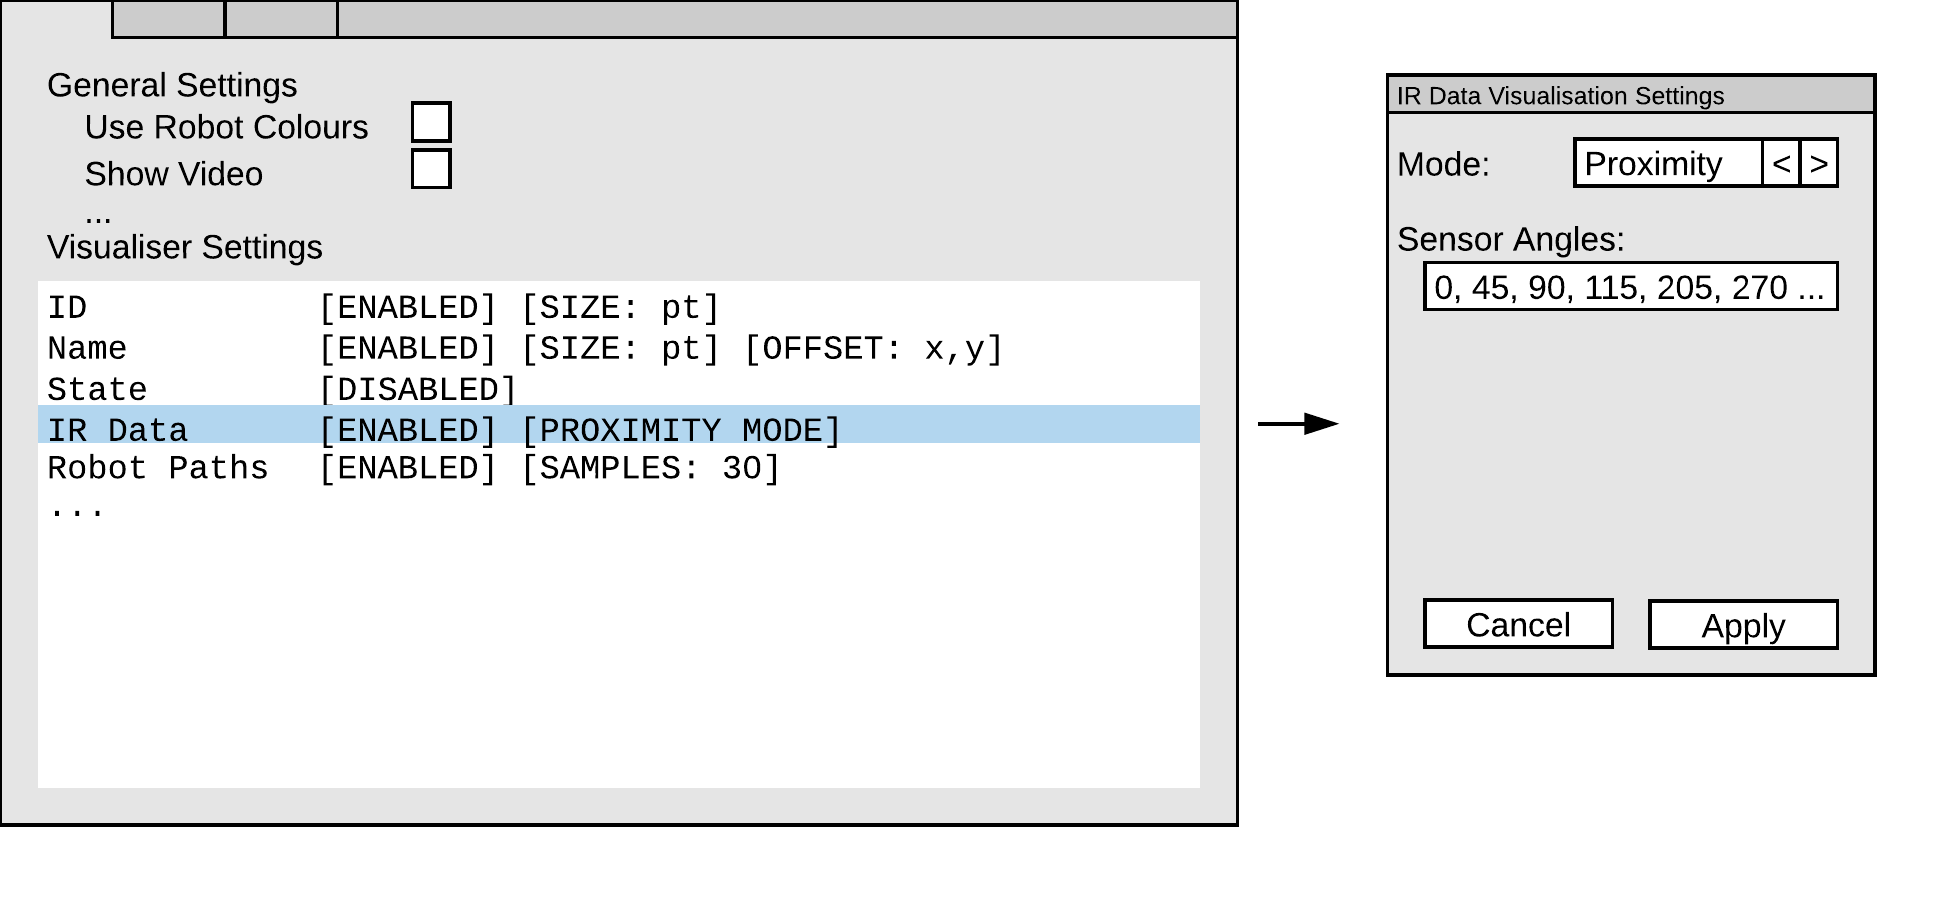
\includegraphics[scale=1]{Figures/VisualiserSettingsTabDesign.png}
	\decoRule
	\caption[Visualiser Settings Tab Design]{The initial UI design for the visualiser settings tab, and pop-up visualisation settings windows.}
	\label{fig:VisualiserSettingsTabDesign}
\end{figure}

\subsection{Data Visualisation Designs} \label{DataVisualisationDesigns}

As well as designing layouts for some of the more complex individual UI elements, designs were also created for some of the graphical overlays that would be shown within the visualiser. The best way to visualise the data could not be determined prior to implementing the visualiser, hence a number of variations for the overlays of each type were generated. These could then be tried in practice to determine which were the most effective. Figure \ref{fig:OverlayDesigns} shows a selection of the overlay designs for the key data visualisation types, with the data visualisation shown in orange. Each row of the figure shows the visualisation design for a different type of data. The details of these designs are as follows.

\begin{description}
\item [Row 1.] Shows the representational 'robot' (a grey circle with an ArUco tag on top) with no overlay applied, for reference purposes. 

\item [Row 2.] Shows three options for the position overlay, including circular and square outline designs, and a filled circle design. It was thought that the filled circle might be easier for a user to see, but had the downside of obscuring the robot, whereas the outline designs might be more difficult to see depending on the width of the lines.

\item [Row 3.] Shows three options for the direction overlay. The first uses a simple line on top of the robot, from its centre outward, indicating its direction. The second develops on the first with an arrow, which might potentially add clarity, but would be more difficult to render at small sizes. The third also uses an arrow, rendered slightly away from the robot. This arrow could rotate to match the robot's orientation, but maintain the same positional offset, or it could simply rotate with the robot about its centre point. Offsetting the arrow makes the shape clearer as it does not overlap the robot, however in practice it could overlap other overlay elements, reducing the clarity of both. 

\item [Row 4.] Shows three options for the positioning of text overlays, including above and below the robot, and offset both vertically and horizontally. Text overlays are unlikely to be readable if rendered directly on top of the robot, and will always be prone to overlapping other elements if rendered with an offset. 

\item [Row 5.] Shows two possible IR data overlay designs. The first uses lines to display the sensor values, where the lines are oriented to face in the direction of the sensors, and their lengths vary with the relevant sensor value. If the lines were to vary inversely with their related sensor values this could be used as an approximate proximity display. The second design shows a `heat map' style overlay, where the values of the sensors are indicated by boxes that change colour in relation to the relevant sensor value. 

\item [Row 6.] Shows three variations of the robot path overlay design, including smooth and stepped lines as well as solid and dotted variants. A smoother path line would likely require more data to be stored, which might be a disadvantage.
\end{description}

\begin{figure}
	\centering
	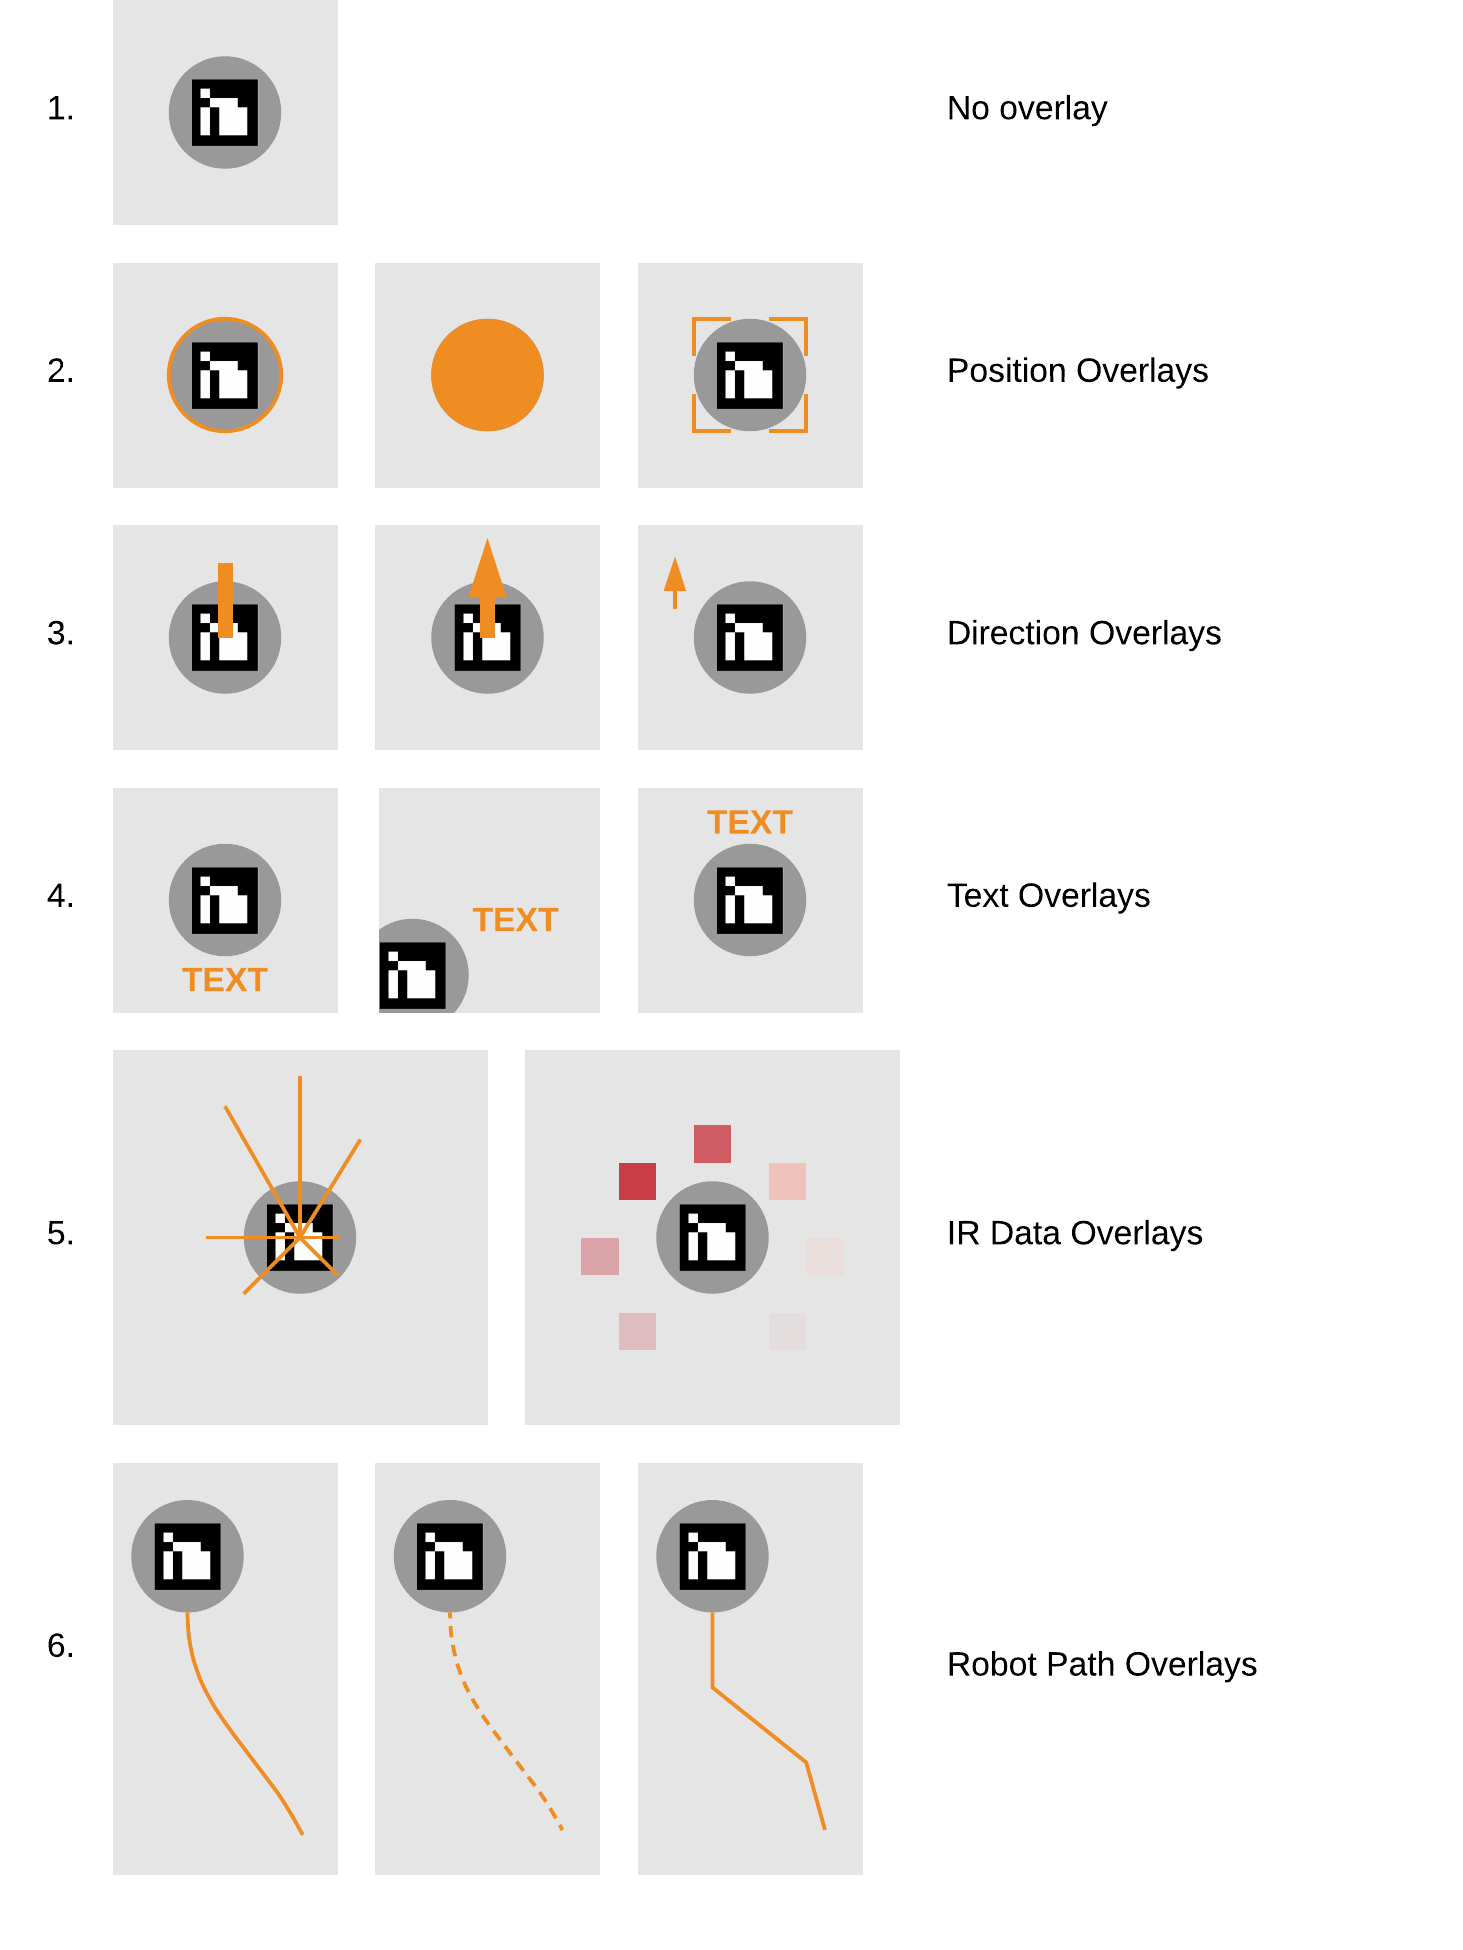
\includegraphics[scale=1]{Figures/OverlayDesigns.png}
	\decoRule
	\caption[Visualiser Overlay Designs]{A selection of the designs for visualiser overlays, for a number of data types.}
	\label{fig:OverlayDesigns}
\end{figure}

%----------------------------------------------------------------------------------------

\section{Summary}

In this chapter the design of the application was described, including details of both the software architecture design and the user interface design. The software architecture is designed with OOP practices practices in mind, and is based on the MVC software architecture pattern. Details of the internal structural design of two of the key functional components - the \textit{Data Model} and the \textit{Visualiser} - were also presented. The user interface design included details of the three main interface panels and their intended functions, as well as specific designs for the contents of different tabs within each panel. A number of possible designs for each of the different data visualisation overlays to be displayed in the visualiser were also presented. With these designs in place the implementation stage could begin to realise the application in code, as discussed in the next chapter.
% Chapter 9

\chapter[Implementation]{Implementation} % Main chapter title

\label{Chapter9} % For referencing the chapter elsewhere, use \ref{Chapter9} 

%----------------------------------------------------------------------------------------

This section gives details of the implementation phase of the project, including descriptions of how parts of the system function, information regarding the development process and explanations for some of the key decisions made regarding the implementation.

\section{Overview}
The system was implemented closely following the design laid out in chapter \ref{Chapter8}, and is comprised of two parts; the main computer software application (referred to henceforth as `the application') and a collection of software routines designed to be included within the code on the robots, which form an `application programming interface' (API) . This API (referred to as the 'robot side code' or 'robot side API') provides the developer with functions to send data from the robot back to the application, and contains routines for handling the networking requirements to achieve this, and for correctly formatting the data. Details of this robot side API are provided in section \ref{RobotSide}. Both parts of the system implementation are fully independent. The application can be run on its own and receive data from another source, provided that this data correctly follows the format outlined in section \ref{DataTransferFormat}. The robot side code could be used to send data to another host, provided that the robot used the correct target IP address and port number, and again provided that the host could correctly interpret the data format. The application is the much larger of the two system parts, and therefore will be the focus of the majority of this implementation chapter.

Figure \ref{fig:UI} shows the user interface for the application as it is seen at start-up. This can be compared to figures \ref{fig:UILayout} and \ref{fig:UIExample} to see the relationship to the user interface design. The key features of the application can be seen in this image, including the video feed augmented with information about the three visible robots, including position, direction, ID number, and for the selected robot name and current state. The robot list panel is also visible on the right hand side, showing the IDs and names of the known robots, and which is currently selected. Finally the data panel can be seen at the bottom of the application, currently set to the overview tab, providing more detailed information about the selected robot. More detailed information about the implementation of the UI itself can be found in section \ref{UserInterfaceImplementation}.

\begin{figure}
	\centering
	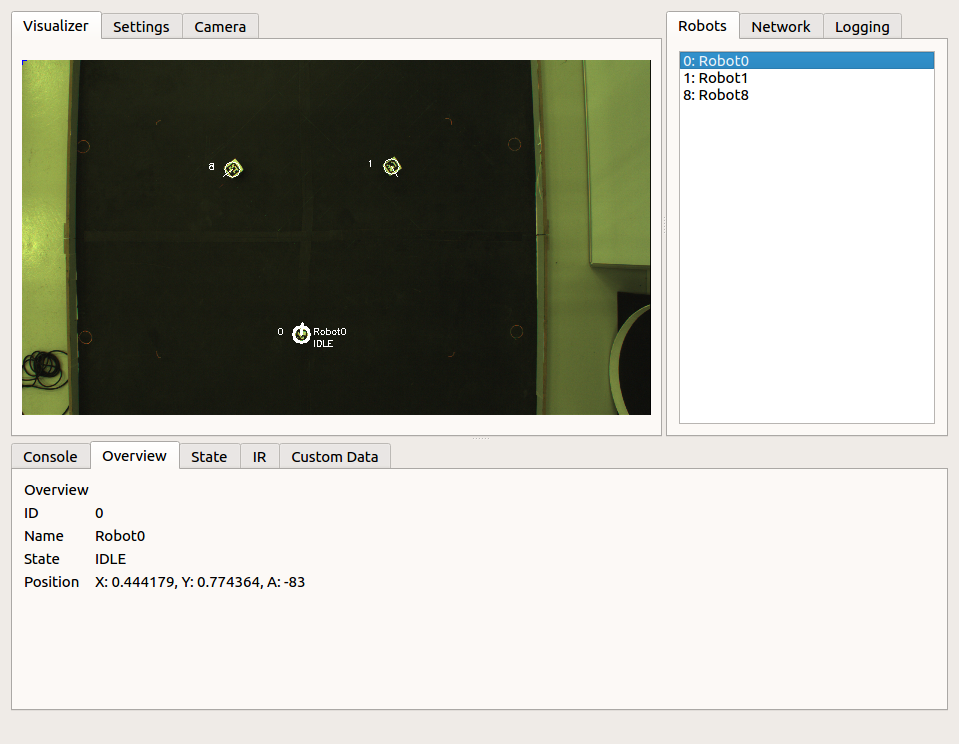
\includegraphics[scale=0.4]{Figures/ApplicationScreenshotOverview.png}
	\decoRule
	\caption[Application User Interface]{The user interface for the application.}
	\label{fig:UI}
\end{figure}

\section{Application Framework Selection}
Developing computer software applications often involves implementing a large amount of the same low level functionality, regardless of the application. This includes low level back end functionality such as event management and dissemination, standard constructs such as timers and threads, as well as standard user interface elements such as windows, menus, panels, lists, tables, buttons and many more. It is clear that these functionalities are independent of the purpose of the application being developed, and implementing them from scratch for each new application would require a huge amount of time, and therefore be extraordinarily inefficient. For this reason the vast majority of modern software is created using some kind of application programming framework. The purpose of these frameworks is to provide the common, low level application functionality in the form of an API, which the developer can then leverage to develop their specific application. The API will usually include a number of classes to define the common UI elements, and a hierarchical tree- or node-based structure the developer can populate with these individual elements to create their desired UI. Most computer applications are event driven; when the user provides some kind of input such as a click or a key press an event is generated. The event generated will be different depending on which UI component the user was interacting with. This event then needs to be disseminated through the application in order to trigger the correct functionality. Most application programming interfaces will handle the generation and dissemination of these events, allowing the developer to `\textit{register}' code to be executed in response to specific events. The developer can therefore simply focus on implementing the functionality that is unique to their application.

Most modern application frameworks contain a wide variety of features in addition to those responsible for the UI and event management. These can include everything from low level components such as timers, input/output (I/O) interfaces, and networking components, to higher level multimedia handlers such as video and audio players, and rich HTML viewers. Frameworks also might include classes for creating data models which can be easily mapped to more complex user interface elements such as responsive tables.

Selecting an appropriate framework to use as the basis for this application was one of the first steps in the implementation process. All of the available frameworks have different benefits and limitations, and target a variety of different platforms, operating systems, and languages. During the design phase it was determined that the application should be implemented in C++, for reasons discussed in section \ref{SoftwareArchitectureDesign}. This therefore eliminated a number of frameworks, such as the Oracle Application Development Framework which is specific to the Java language, and Microsoft's .NET framework, which is C\# specific. The application also needed to run on the server connected to the tracking camera, which runs a Linux operating system. This therefore ruled out any windows specific framework, including one of the most widely used C++ frameworks, the Microsoft Foundation Class Library (MFC).

\subsection{The Qt Framework}
It was determined that the `\textit{Qt}' application framework was the most suitable for this application, as it provides support for cross-platform compilation, including Linux, and was implemented natively in C++. A number of factors, in addition to the target platform and language, influenced this decision. The framework is fairly widely used, and therefore has a well-tested, refined, and mature API, with a good body of documentation available. It provides a comprehensive library of classes for a range of common application functionalities, including GUI front-end and low level back-end components. The framework also includes built in support for multi-threading, and a structured `\textit{signals and slots}' system for sending event notification and moving data between components and across threads. For an application such as this, with a number of external data sources in addition to the user input and a multi-threaded design, this was determined to be a highly beneficial feature which could reduce development complexity significantly. Furthermore previous experience with Qt outside of this project had been positive, and meant a smaller learning curve would be necessary to get started developing the application. For non-commercial projects Qt is available free of charge, making it a good fit for an academic project.

The following primary features of the Qt application framework were used within this project:

\begin{itemize}
 \item Standard GUI components and layout management classes used to create the majority of the user interface.
 \item Event management system to handle user input events.
 \item `\textit{QTimer}' component to implement timers and recurring events, such as camera polling.
 \item `\textit{QThread}' API to partition the application components into threads.
 \item `\textit{Signals and Slots}' system for inter-component and inter-thread signalling and data transfer.
 \item `\textit{QPainter}' component for rendering custom user interface elements.
\end{itemize}

%----------------------------------------------------------------------------------------

\section{Source Code}
The system source code is implemented in two groups of files; a collection of C++ source and header files which make up the main application, and a smaller collection of C++ source and header files which handle the robot-side portion of the system. In addition to its source files the main application also relies on a number of other files which are used by the Qt system to define the user interface layout, and manage the build process. Table \ref{tab:CodeFiles} details the names and purposes of all files within the main application. Table \ref{tab:RobotCodeFiles} details the files that make up the robot side API.

\begin{longtable}{ l p{10cm} }
\caption[Application Code Files]{Source code and tertiary files that make up the main application.}\\
 File & Purpose\\ 
 \hline
 main.cpp & The entry point for the application. Instantiates the MainWindow class.\\
 mainwindow.cpp, .h & The core class, contains the entry point for the application and controls the set up and tear down processes and handles UI events within the main window.\\
 mainwindow.ui & Describes the user interface layout in a XML-like format. Used by the Qt framework to construct the UI.\\
 datamodel.cpp, .h & The top level class encapsulating the full data model. Maintains a list of RobotData objects.\\
 robotdata.cpp, .h & A class encapsulating the data of a single robot, including ID, position, state, sensor data and user data.\\
 datathread.cpp, .h & This class contains all routines for receiving data from the robots via wifi, and is designed to be run on a thread of its own.\\
 cameracontroller.cpp, .h & The high level class encapsulating the routines and data related to the tracking camera. This class is designed to be independent of the camera hardware being used.\\
 machinevision.cpp, .h & A lower level class encapsulating routines for interfacing with the camera hardware.\\
 visualiser.cpp, .h & This class encapsulates the visualiser GUI object, and is implemented to conform the Qt framework as a custom extension to the QWidget class. Also contains routines for applying the video augmentations as per the current visualiser settings.\\
 viselement.h & Contains an abstract class definition for a single visualiser settings element. These elements are used to define how specific elements of the video augmentation are rendered, and also contain settings and variables relevant to this task. \\
 vis*.cpp, .h, .c & Classes beginning with the `\textit{vis}' prefix derive from the VisElement abstract class and contain routines for rendering the visualisation for one type of data. The latter part of the class name identifies which data type is targeted.\\
 irdataview.cpp, .h & A custom GUI object, derived from QWidget, which displays the raw IR sensor data as a bar graph in the data window.\\
 settings.cpp, .h & Encapsulates the general application settings and routines for changing their values according to user input.\\
 log.cpp, .h & Encapsulates the routines for logging events and data to text files.\\
 util.cpp, .h & Contains static utility functions used in various places throughout the application code.\\
 *settingsdialog.cpp, .h & Classes ending with the `\textit{settingsdialog}' suffix describe dialog windows for adjusting the settings related to the visualisation of specific data types, identified by the first part of the class name.\\
 robotinfodialog.cpp, .h & Defines a dialog window which displays meta information about a specific robot, and provides controls to delete that robots data from the data model.\\
 addidmappingdialog.cpp, .h & Defines a dialog window which can be used to add a non-standard ID mapping.\\
 testingwindow.cpp, .h & Defines a dialog window for running and displaying the results of the data model unit tests.\\
 appconfig.h & Contains pre-processor definitions for controlling inclusion/exclusion of code segments.\\
 SwarmDebug.pro & Used by the Qt framework to build the application. Directs to the necessary code files and libraries.\\
 \bottomrule\\
	
 \label{tab:CodeFiles}
\end{longtable}

\begin{longtable}{ l p{10cm} }
\caption[Robot-side Code Files]{Source code files that make up the robot side API.}\\
 File & Purpose\\
 \hline
 debug\_network.cpp & This file encapsulates networking functionality for communicating with the debugging system. Contains routines for sending data of specific types, as well as for sending raw packets.\\
 debug\_network.h & Header file for the debugging system network interface. Also contains definitions for data type identifiers.\\
 \bottomrule\\
	
 \label{tab:RobotCodeFiles}
\end{longtable}

%----------------------------------------------------------------------------------------

\section{Data Model} \label{DataModel}
The data model forms the core of the `\textit{unseen}' or back end code for the application - code that does not directly influence the interface seen by the user. For each robot being tracked by the system, the data model is required to store the information related to that robot. This is done in a structured manner, such that other parts of the application can query specific data within the model easily. The contents of the data model are updated whenever new data arrives, and are consulted when rendering the user interface. Section \ref{DataModelDesign} describes the design of the data model and it's hierarchical structure. The implementation follows this design closely, with the \textit{DataModel} class contained in \textit{datamodel.cpp / .h} encapsulating the top level data model container, and the individual robot data object encapsulated in the \textit{RobotData} class in \textit{robotdata.cpp / .h}. 

The \textit{DataModel} class uses a standard C++ vector to maintain a list of \textit{RobotData} objects. Each of these \textit{RobotData} objects describes one robot that is currently known to the system. The list is ordered based on the robot ID of each entry, and is sorted after each new insertion. The \textit{DataModel} class provides convenience functions for data retrieval functionality, such as retrieving a robot's data given its ID. It also provides a function for entering new data into the model, which inherits the properties of a `\textit{slot}' within the Qt framework, allowing it to be called from other threads. Each new data packet received from the network is routed to this slot, as well as position data obtained from the tracking system. All data is supplied in the form of a string in one of the packet formats described in section \ref{DataTransferFormat}. Code within the data model class then handles interpreting the string, determining its purpose and the source robot, separating out the data and updating the relevant robot within the model. Whenever data arrives from a previously unknown robot, this code handles creating a new \textit{RobotData} object, and adding it to the list.

The \textit{RobotData} class encapsulates the data for a single robot. This includes a large number of individual data points, in a number of different formats. Table \ref{tab:RobotDataContents} describes these data points.

\begin{longtable}{ l l p{8cm} }
\caption[Robot Data Contents]{The contents of the \textit{RobotData} class.}\\
 \hline
 Data Point & Type & Description\\
 \hline\\
 Robot ID & Integer & The numerical ID of the robot, used by the tracking system and when transmitting data.\\
 Robot Name & String & The name associated with this robot. Set by the user when programming the robot, and reported in watchdog packets. \\
 State & String & The current state of the robot. \\
 Known States & List of strings & A list of all states the robot has previously reported. \\
 Position & 2D Vector & The current position of the robot expressed as a proportional coordinate vector. \\
 Angle & Integer & The current angle of the robot in degrees. \\
 Colour & OpenCV Scalar & The colour used for this robot in the visualiser, if colours are enabled, expressed as an OpenCV Scalar struct in RGB format. \\
 IR Data & Array of Integer & The most recent IR sensor readings for this robot. One value per sensor. \\
 Background IR Data & Array of Integer & The most recent background IR sensor readings. One value per sensor. \\
 Custom Data & Key Value Map & All custom user data. Stored as a map of key value pairs. \\
 
 \label{tab:RobotDataContents}
\end{longtable}

In addition to this data, the class also maintains a list of recent state transitions, and a short term history of the robot's position. The state transition list uses a custom structure to store the state before the transition, the state after the transition, and the time the transition occurred. A fixed size array of these custom structures is maintained and updated each time a state transition occurs, acting as a first-in first-out (FIFO) queue. The position history is stored in a similar fashion, using a fixed size array of coordinate pairs, which is updated every Nth position update. This interval can be configured by the user, with a lower interval giving a higher resolution but a shorter history, and vice versa for a higher interval.

%----------------------------------------------------------------------------------------

\section{Video Feed and Tracking System} \label{VideoFeedAndTrackingSystem}
The code relating to retrieving images from the machine vision camera and running the ARuCo tag tracking algorithm can be found in the files \textit{cameracontroller.cpp / .h} and \textit{machinevision.cpp / .h}. This code is run on the separate camera thread, in order to maximise application performance and ensure responsiveness in the event that the camera driver blocks execution whilst retrieving the next frame. The \textit{CameraController} class handles the higher level operations such as running a timer to periodically poll the camera driver for the next image, supplying the driver with the correct dimensions for the image to be resized to in order to fit within the available space in the UI, and converting the image itself and the tracking data into formats which can be passed back to the main thread and used in the UI and data model respectively. The application threading is handled through the use of the Qt framework's \textit{QThread} API, and communication between threads utilises the framework's `\textit{signals} and \textit{slots}' feature, which allows components on different threads to send and receive data in a managed, thread-safe manner. The \textit{CameraController} class therefore utilises two signals; one for emitting the camera image data, and another for emitting the robot position data. At initialisation time the application's core class, \textit{MainWindow}, connects these signals to matching slots within the \textit{Visualiser} and \textit{DataModel} classes respectively.

The \textit{MachineVision} class handles the lower level operations related to the camera and the tracking system, including setting up the camera driver, retrieving and resizing individual images from the camera and running the ARuCo tag detection algorithm. The ARuCo software is included as an additional component of the OpenCV image processing library, and provides the function `\textit{aruco::detectMarkers}' which will run the tag detection algorithm on a given OpenCV image. For each tag detected in the image the ARuCo algorithm returns the pixel coordinates of the four corners of the tag. The \textit{MachineVision} class includes code to average these four coordinates, acquiring a central pixel coordinate, and then convert this to a 'proportional' coordinate; two numbers between 0 and 1 which represent the horizontal and vertical components of the position as a proportion of the full height and width of the image respectively. This ensures that the robot positions can still be correctly displayed after the image has been resized, without having to maintain information related to the resizing operation. The angle the robot is facing is also calculated. This is done by first calculating the position of the fourth corner, as a coordinate relative to the position of the third, and then applying an arctangent function to this coordinate. This angle is then converted to degrees and stored as an integer in order to reduce complexity, as a precision greater than one degree was not deemed necessary.

%----------------------------------------------------------------------------------------

\section{Networking}
The networking requirements of the system were relatively simple, and can be summarised as follows:

\begin{enumerate}
	\item Must utilize a WiFi network.
	\item Must allow a large number of sources to transmit data to a single host
	\item Must allow for frequent transmission of small packets of data
\end{enumerate}

WiFi networks utilise the standard Internet Protocol (IP) network layer protocol. There are two commonly supported transport layer protocols which run on top of IP, the Transmission Control Protocol (TCP) and the User Datagram Protocol (UDP). TCP is a managed and delivery-error checked protocol, and therefore guarantees that packets will be transmitted in the correct order, with lost packets being retransmitted. This adds overheads such as acknowledgements to the protocol, and requires an established 'connection' in order to function correctly. TCP also operates a queueing system, whereby packets for transmission are held until a number of them are ready, and can therefore be grouped together and sent. UDP, by contrast, does not error check the delivery of packets, making no guarantees that a packet will be received, or that packets will be received in the correct order, removing the need for an established connection and reducing the overheads involved. Packets can therefore be sent from any application to any target IP address and port on the network, without first establishing a connection with another application. Packets are also sent immediately, with no queueing system in place It was determined that the User Datagram Protocol (UDP) would be the most suitable for this system, for a number of reasons. The connection requirements of TCP would require the to form a connection with application each robot prior to transmitting data, which would add unnecessary complexity. Using UDP also ensured that the packets were transmitted immediately, reducing the potential for latency in the system. The lack of delivery checking was not considered an issue, as the robots would be transmitting updates frequently enough that a single lost packet would not cause a significant issue.

Code relating to the networking functionalities of the application is contained in the files \textit{datathread.cpp / .h}, which encapsulate the \textit{DataThread} class. This class is run on a dedicated thread to ensure that potentially blocking operations do not impact application performance. This class contains routines for dealing with the low level network requirements, such as establishing a socket through which to receive data packets from the robots, and continually listening on this socket for new data. All socket operations are implemented using structures and definitions from the standard C++ networking libraries. Data received from the robots is passed to the main application thread through a Qt signal, using the Qt signals and slots interface in the same manner as described in section \ref{VideoFeedAndTrackingSystem}. The main application class, \textit{MainWindow}, connects this signal to the appropriate slot in the \textit{DataModel} class. The application side networking is configured in the \textit{network} tab of the right-hand panel of the user interface. The user is able to enter a desired port number on which to receive data, and can begin listening for packets on this port by pressing the `\textit{start listening}' button.

Within the robot side API, the networking functionality is implemented in a very similar way. The initialisation function establishes a target socket based on a supplied IP address and port. This should match the IP address of the computer or server running the main application, and the port chosen by the user within the main application. When any of the functions for sending specific data packets are called, the data is then sent to this target socket. All socket operations are again implemented using the standard C++ networking libraries.

%----------------------------------------------------------------------------------------

\section{Data Transfer Format} \label{DataTransferFormat}
In order for the application to interpret and use data received from the robots, a common format for exchanging data needed to be defined, and used correctly at both ends of the communication link. A number of different options were considered for achieving this, ranging from super-lightweight custom packets using the minimum number of bytes, to established existing solutions such as the JSON data interchange standard. The primary concerns when making this decision were a desire to minimise any overhead in terms of extra code needed on the robot side, as the robots have limited memory, and to ensure the format remained as simple as possible, so that future extensions to the system, such as implementations for other robots, could be programmed with relative ease. It was ultimately decided not to use JSON, to avoid the need for any additional code libraries to be stored in the robot's memory, and to instead use a custom simple string-based packet format. All data to be transmitted from the robot to the application is therefore converted to a simple string which is then transmitted in the data packet. As well as containing the data, the string must identify the robot and describe the type of data within. The format for these strings is defined as three sections separated by space characters. The first section contains the numerical ID of the robot sending the packet. The second contains a number identifying the type of data contained in the packet. The last section contains the packet data, and has a variable format, depending on the packet's type. Figure \ref{fig:DataFormat} gives a visual representation of this format. Table \ref{tab:DataFormat} describes the purpose of each packet type, and describes the format of the `packet data' section for each.

\begin{figure}
	\centering
	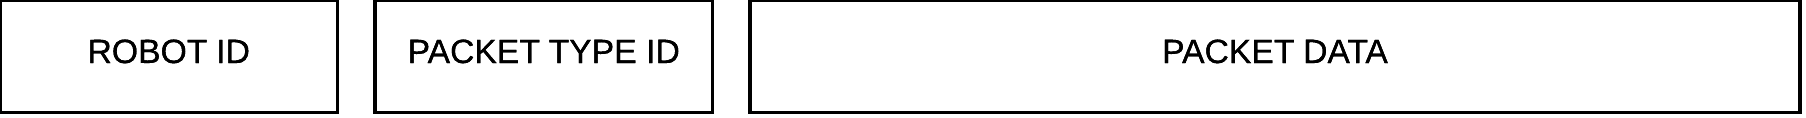
\includegraphics[scale=0.3]{Figures/DataFormat.png}
	\decoRule
	\caption[Data Format]{The general format for each data packet.}
	\label{fig:DataFormat}
\end{figure}

\begin{longtable}{ l p{12cm} }
\caption[Data Format]{The format of the data section and the purpose of each packet type.}\\
 \hline
 \multicolumn{2}{p{12cm}}{\textbf{Watchdog Packet}}\\
 \hline
 Type ID & 0 \\
 Format & [ROBOT NAME]\\
 Purpose & Sent periodically to inform the application that the robot is still active. Also contains the robot's name, as should be displayed in the application.\\
 
 \hline
 \multicolumn{2}{p{12cm}}{\textbf{State}}\\
 \hline
 Type ID & 1 \\
 Format & [CURRENT STATE]\\
 Purpose & Informs the application of the robots current state.\\
 
 \hline
 \multicolumn{2}{p{12cm}}{\textbf{Position}}\\
 \hline
 Type ID & 2 \\
 Format & [X POSITION] \_ [Y POSITION] \_ [ANGLE]\\
 Purpose & Provides the application with a robot's position and orientation. This data is not sent by the robot, but instead comes from the tracking code.\\
 
 \hline
 \multicolumn{2}{p{12cm}}{\textbf{IR}}\\
 \hline
 Type ID & 3 \\
 Format & [SENSOR 1 DATA] \_ [SENSOR 2 DATA] \_ ... [SENSOR N DATA] \\
 Purpose & Contains a robot's infra-red sensor readings. Each sensor value is separated by a space, and the packet can contain as many values as the robot has IR sensors. \\
 
 \hline
 \multicolumn{2}{p{12cm}}{\textbf{Background IR}}\\
 \hline
 Type ID & 4 \\
 Format & [SENSOR 1 DATA] \_ [SENSOR 2 DATA] \_ ... [SENSOR N DATA] \\
 Purpose & Contains a robot's background infra-red sensor readings. Formatted the same as the standard IR data packet.\\
 
 \hline
 \multicolumn{2}{p{12cm}}{\textbf{Message}}\\
 \hline
 Type ID & 5 \\
 Format & [MESSAGE STRING]\\
 Purpose & This packet allows any general message to be sent from the robot to the application, and will be displayed in the application console and recorded in the logs. \\
 
 \hline
 \multicolumn{2}{p{12cm}}{\textbf{Custom Data}}\\
 \hline
 Type ID & 6 \\
 Format & [KEY] \_ [VALUE]\\
 Purpose & Contains a piece of custom user data, in the form of a key value pair. \\
	
 \label{tab:DataFormat}
\end{longtable}

%----------------------------------------------------------------------------------------

\section{User Interface} \label{UserInterfaceImplementation}
The user interface has been implemented using the Qt GUI framework. The layout for the interface is defined in \textit{mainwindow.ui}, a file generated by the Qt interface designer application to describe the structure and layout of the interface components in an XML based format. The Qt framework uses a standard event-driven interface paradigm, where events are generated when the user interacts with the interface, and code is used to define specific routines to execute in response to relevant events. The routines for handling interface events can be found in \textit{mainwindow.cpp / .h}, and are usually prefixed with the term `\textit{on\_}'. For example, the function `\textit{on\_actionExit\_triggered}' is called when the `Exit' action is selected from the menu, and instructs the application to close.

[INDIVIDUAL UI ELEMENTS w/ SCREENSHOTS]

In addition to the main user interface, a number of extra `dialog' windows are used to provide the user with access to the settings of each visualisation element, if settings are available. These dialog windows are defined in the files  \textit{idsettingsdialog.cpp / .h, pathsettingsdialog.cpp / .h} and \textit{proximitysettingsdialog.cpp / .h}. Dialog windows are a commonly used tool within application programming. They act as pop-up windows which usually require the user to either confirm or cancel some change. In this case the dialog windows present controls for changing specific visualisation settings, and the user can then either apply their changes or cancel them using the standard accept/reject buttons at the bottom of the window.

%----------------------------------------------------------------------------------------

\section{Visualiser}
The 'visualiser' is the name given to the custom user interface component that renders the augmented video feed. Implementing this component was key to satisfying the portion of the project aims related to augmented reality, and it forms one of the most visible elements of the system. The main visualiser component is defined in the \textit{Visualiser} class (\textit{visualiser.cpp / .h}), and a number of extra classes are used to define the associated settings and routines for visualising specific data types (\textit{VisConfig, VisID, VisName, VisState, VisPosition, VisDirection, VisProximity, VisPath}). Section \ref{VideoFeedAndTrackingSystem} describes the process of retrieving images from the camera and tracking the robots. The image data then arrives at the visualiser via a Qt slot function. At this stage the image is augmented based on the data in the data model, by iterating over the list of robots, and for each one iterating over the list of data visualisations, calling the render function for each. These render functions take the image and the current robot's data as arguments, and then add the relevant graphical representation to the image using the drawing functions within the OpenCV image processing library.

It was decided that an individual class would be implemented for each type of data visualisation, derived from the abstract class \textit{VisElement}. The aim was to make the visualisation process simpler to manage, and to follow object oriented practices, making it easier for new visualisation types to be added without modifying the underlying system. This also allows each data visualisation object to maintain its own settings, so that the visualiser component itself need not be aware of the details of the configuration of each data visualisation element. Instead each data visualisation element simply checks it's own configuration when it's render function is called.

The rest of the code in the \textit{Visualiser} class relates to embedding the OpenCV image within a Qt UI widget, and tertiary functionality such as detecting clicks within the image frame, and retrieving the frame's size. The OpenCV to Qt image conversion is done by instantiating a QImage instance directly from the internal pixel data of the OpenCv image. This QImage is then drawn onto the widget.

\subsection{Data Visualisations}
The visualiser supports a number of specific data visualisations:

\begin{enumerate}
 \item Displaying robot positions.
 \item Displaying robot 'orientations' by highlighting their forward directions.
 \item Displaying the ID of a robot as text close to its position.
 \item Displaying the name of a robot as text close to its position.
 \item Displaying the current state of a robot as text close to its position.
 \item Displaying a graphical representation of a robot's IR sensor data.
 \item Displaying the recent path a robot has taken as a line behind the robot.
\end{enumerate}

Each visualiser element can be enabled and disabled via the settings tab. Some of the visualisations have more complex settings, which can be accessed be double clicking the specific element in the visualisations list, also in the settings tab. Figure  shows the text based visualisations. Figure  shows the position and orientation visualisations. The IR sensor data visualisation is more complex, and offers a number of configuration options. The visualisation can either display in 'proximity mode' or 'heat mode'. In proximity mode lines are drawn in the direction each sensor is facing to approximate the proximity of the surface reflecting the IR pulses. This line therefore varies inversely with the value of the sensor. This mode can be seen in figure . In heat mode the IR sensors are represented as small blocks positioned around the perimeter of the robot. The size of the blocks and their colour varies in relation to their corresponding sensor value, as can be seen in figure . Both modes position their visualisations to correspond with the individual sensor positions, and this can be adjusted by the user via the IR visualisation settings dialog. The settings dialog also allows the user to decide whether IR data should be displayed for all the robots, which can overwhelm the display, or just the selected robot. The path visualisation can be seen in figure , and can also be configured to display for all robots or only the selected one. The user can also configure the interval between the position samples (as discussed in section \ref{DataModel}) via the settings dialog, which effects the smoothness and length of the path line.

[SCREENSHOTS]

%----------------------------------------------------------------------------------------

\section{Robot Side API} \label{RobotSide}
The robot side API is defined in `\textit{debug\_network.cpp / .h}' as a single class, \textit{DebugNetwork}. The contents of the \textit{DebugNetwork} class are described in table \ref{tab:RobotAPI}.

\begin{longtable}{ l l p{8cm} }
\caption[Robot API]{The contents of the \textit{DebugNetwork} class the forms the robot side API.}\\
 \hline
 \multicolumn{3}{l}{\textbf{Variables}} \\
 \hline
 Name & Type & Purpose\\
 \hline\\
 socket\_ready & Boolean & Indicates whether the socket has been created successfully, and it ready to be used.\\
 sock\_in & Struct & A structure defining the target socket.\\
 sock\_fd & Integer & Identifies the socket on the local machine (robot).\\
 robot\_id & Integer & The numerical ID of this robot. Set at initialisation time. Inserted to the header of each packet to identify the sender.\\
 \hline
 \multicolumn{3}{l}{\textbf{Functions}} \\
 \hline
 Name & Return Type & Purpose\\
 \hline\\
 init & Void & Initialises the class by setting up the socket and setting the ID for this robot. Requires a port number, a target host IP address and the robot ID as arguments. \\
 destroy & Void & Shuts down the socket. \\
 sendData & Void & Sends a given string as a raw data packet. \\
 sendWatchdogPacket & Void & Constructs and sends a watchdog packet. Requires the robot name to be provided as an argument. \\
 sendStatePacket & Void & Constructs and sends a state packet. Requires the current state to be provided as an argument string. \\
 sendIRDataPacket & Void & Constructs and sends an IR data packet. Requires the data be arranged into an array, and takes a pointer to the first element and a size value as parameters. Also takes an extra boolean parameter which can be set to true to indicate that this packet should be identified as backgroud IR data.\\
 sendLogMessage & Void & Constructs and sends a message packet to display a message in the application console and logs. The message string is supplied as an argument.\\
 sendCustomData & Void & Constructs and sends a custom data packet. The key value pair are supplied to this function as two argument strings.\\
 getRobotID & Integer & Returns the numerical robot ID, as currently set. \\
 setRobotID & Void & Sets the numerical robot ID based on an integer argument. \\
 
 \label{tab:RobotAPI}
\end{longtable}

In order to utilize this API a user can modify their robot controller code to include the \textit{debug\_network.h} header file, call the \textit{init} function at start-up time, and then call the various packet and data functions whenever necessary. The user is therefore in charge of how frequently data is transmitted, and can decide whether to simply send updates to the application when the robot's data changes, or to transmit a fixed quantity of data every control step. It was potentially possible for the API to handle all data reporting in the background, without requiring the user to specify when to transmit data in the controller code, however this approach was not taken for a number of reasons. Firstly it limits the control and flexibility available to the user. Each swarm system is different, and may have different requirements, hence the API should allow the developer to make decisions regarding data reporting which are right for their specific case. It would also limit the portability of the API, as a more automatic system would likely have to hook into the lower level robot drivers, meaning much greater changes would be necessary to port the code to a different robot. Furthermore by allowing the user to have complete control over when and how frequently data is transmitted they are able to manage the amount of traffic they are putting on their network, potentially mitigating congestion issues with very large swarms. Finally allowing users to control the moments within the code when data is reported to the debugging system was deemed to be a more intuitive system, especially as many developers are already familiar with the concept of using `print' statements within code to display debugging messages in a console.

%----------------------------------------------------------------------------------------
% Chapter 10

\chapter[Testing and Evaluation]{Testing and Evaluation} % Main chapter title

\label{Chapter10} % For referencing the chapter elsewhere, use \ref{Chapter10} 

%----------------------------------------------------------------------------------------

\section{Overview}


%----------------------------------------------------------------------------------------

\section{Continuous Integration Testing}


%----------------------------------------------------------------------------------------

\section{Validation Testing}


%----------------------------------------------------------------------------------------

\section{User Evaluation}

\subsection{Method}
\subsection{Results}
\subsection{Analysis}

%----------------------------------------------------------------------------------------
% Chapter 11

\chapter[Future Work]{Future Work} % Main chapter title

\label{Chapter11} % For referencing the chapter elsewhere, use \ref{Chapter11} 

%----------------------------------------------------------------------------------------

\section{Use within the York Robotics Laboratory}


%----------------------------------------------------------------------------------------

\section{Platform Development}


%----------------------------------------------------------------------------------------

\section{Integration with Tablet Application}


%----------------------------------------------------------------------------------------

\section{Integration with ARGoS Simulator}


%----------------------------------------------------------------------------------------

\section{Integration with Augmented Reality Hardware}


%----------------------------------------------------------------------------------------
% Chapter 12

\chapter[Conclusion]{Conclusion} % Main chapter title

\label{Chapter12} % For referencing the chapter elsewhere, use \ref{Chapter12} 

%----------------------------------------------------------------------------------------

\section{Overview}


%----------------------------------------------------------------------------------------

\section{Evaluation Against Aims and Objectives}


%----------------------------------------------------------------------------------------

\section{System Limitations}

- Requires code to be added to the robot behaviour to report information, and therefore behaviour may change, especially if this code is removed after debugging.


%----------------------------------------------------------------------------------------

\section{Use Within the York Robotics Laboratory}

One of the key aims of this project was to create a system which is practical, usable, and offers real benefit to swarm robotics developers and researchers. In this capacity it is hoped that the application will continue to be used within the YRL to aid in swarm robotics research and development efforts, and that the application itself will see further development to build upon its core functionality in some of the ways previously mentioned.

%----------------------------------------------------------------------------------------

\section{Value Within the Swarm Robotics Space}


%----------------------------------------------------------------------------------------

%----------------------------------------------------------------------------------------
%	THESIS CONTENT - APPENDICES
%----------------------------------------------------------------------------------------

\appendix % Cue to tell LaTeX that the following "chapters" are Appendices

% Include the appendices of the thesis as separate files from the Appendices folder
% Uncomment the lines as you write the Appendices

% Test Results Appendix

\chapter{Test Results} % Main appendix title

\section{Manual UI Testing Results} \label{app:UITestResults}

\begin{longtable}{ l p{10cm} }
 \hline
 \multicolumn{2}{c}{\textbf{Visualiser Panel Tab System}}\\
 \hline
 \textbf{Purpose} & Allows access to the different tabs within the visualiser panel.\\
 \textbf{Required Functionality} & Must display the names of each different tab. Must allow the user to click on the tabs and thus change between them. The required tabs are the visualiser tab, the visualiser settings tab and the tracking camera settings tab.\\
 \hline
 \multicolumn{2}{p{14cm}}{\textbf{1. Examine UI element visually. Verify that it appears correct. Verify that it contains all elements necessary to satisfy its purpose.}}\\
 \multicolumn{2}{p{14cm}}{The tab bar appears to be visually correct. All required tabs are present and visible.}\\
 \hline
 \multicolumn{2}{p{14cm}}{\textbf{2. Examine all text within the element. Check for errors in both meaning and spelling.}}\\
 \multicolumn{2}{p{14cm}}{The spelling of each tab name is correct. The meaning of each tab name is relatively clear, although 'Settings' is ambiguous, and only related to the visualiser through position and context. Consider renaming this tab to clarify its purpose.}\\
 \hline
 \multicolumn{2}{p{14cm}}{\textbf{3. Verify that all components within the element which perform actions in response to user input operate correctly.}}\\
 \multicolumn{2}{p{14cm}}{Tab selection operates correctly. Clicking any of the tabs changes the panel to display the contents of that tab. This satisfies the required functionality.}\\
 \hline
 \multicolumn{2}{p{14cm}}{\textbf{4. Verify that all components respond quickly to user input.}}\\
 \multicolumn{2}{p{14cm}}{The tab changes immediately when clicked.}\\
 \hline
 \multicolumn{2}{p{14cm}}{\textbf{5. Verify that component actions and functionality do not degrade with extreme use (sustained rapid input, large numbers of input changes, etc).}}\\
 \multicolumn{2}{p{14cm}}{Repeatedly and rapidly changing tabs does not have any detrimental affect on the application.}\\
 \hline
 \multicolumn{2}{p{14cm}}{\textbf{6. Verify that all data displayed within the element is visible, readable, correctly arranged and correctly labelled.}}\\
 \multicolumn{2}{p{14cm}}{n/a.}\\
 \hline
 \multicolumn{2}{p{14cm}}{\textbf{7. Verify that the element behaves sensibly when window resizing occurs, and that it remains usable and data remains visible whenever possible.}}\\
 \multicolumn{2}{p{14cm}}{The tabs are not affected by window resizing. All of the tabs fit within the minimum size of the panel. If the panel is reduced below this size it is minimized, and the tabs are hidden as intended.}\\
 \hline
 \multicolumn{2}{p{14cm}}{\textbf{8. Verify that the element updates promptly when responding to changes in data.}}\\
 \multicolumn{2}{p{14cm}}{n/a.}\\
 \hline
 \textbf{Fixes Required} & Consider changing the text on the visualiser settings tab from 'Settings' to something more informative to improve clarity.\\
 \bottomrule
\end{longtable}
\clearpage

\begin{longtable}{ l p{10cm} }
 \hline
 \multicolumn{2}{c}{\textbf{Visualiser Settings Tab}}\\
 \hline
 \textbf{Purpose} & Displays the current settings for the visualiser and allows the user to change them.\\
 \textbf{Required Functionality} & Must correctly display the current visualiser settings. Must allow the user to adjust the general visualiser settings, and access dialog windows for changing the settings of specific visualisations.\\
 \hline
 \multicolumn{2}{p{14cm}}{\textbf{1. Examine UI element visually. Verify that it appears correct. Verify that it contains all elements necessary to satisfy its purpose.}}\\
 \multicolumn{2}{p{14cm}}{Panel layout appears to be correct. Controls are included to modify all of the required settings.}\\
 \hline
 \multicolumn{2}{p{14cm}}{\textbf{2. Examine all text within the element. Check for errors in both meaning and spelling.}}\\
 \multicolumn{2}{p{14cm}}{All spelling is correct, and the meaning of all text is clear.}\\
 \hline
 \multicolumn{2}{p{14cm}}{\textbf{3. Verify that all components within the element which perform actions in response to user input operate correctly.}}\\
 \multicolumn{2}{p{14cm}}{All the settings controls work correctly. Double clicking on any of the visualiser config elements in the list displays the appropriate settings dialog, if one exists.}\\
 \hline
 \multicolumn{2}{p{14cm}}{\textbf{4. Verify that all components respond quickly to user input.}}\\
 \multicolumn{2}{p{14cm}}{All controls respond immediately to input.}\\
 \hline
 \multicolumn{2}{p{14cm}}{\textbf{5. Verify that component actions and functionality do not degrade with extreme use (sustained rapid input, large numbers of input changes, etc).}}\\
 \multicolumn{2}{p{14cm}}{Rapidly enabling and disabling settings multiple times has no detrimental affect. Disabling and re-enabling the robot colours setting causes the robots to be re-assigned colours randomly, which might be undesired behaviour.}\\
 \hline
 \multicolumn{2}{p{14cm}}{\textbf{6. Verify that all data displayed within the element is visible, readable, correctly arranged and correctly labelled.}}\\
 \multicolumn{2}{p{14cm}}{Information regarding the current settings is readable, correctly arranged and clearly labelled. Detailed settings for each visualiser element are described in text next to the element name.}\\
 \hline
 \multicolumn{2}{p{14cm}}{\textbf{7. Verify that the element behaves sensibly when window resizing occurs, and that it remains usable and data remains visible whenever possible.}}\\
 \multicolumn{2}{p{14cm}}{All text fits within the minimum panel width, and scroll bars are presented when the height becomes too small to display the full visualiser config element list. Resizing is handled gracefully.}\\
 \hline
 \multicolumn{2}{p{14cm}}{\textbf{8. Verify that the element updates promptly when responding to changes in data.}}\\
 \multicolumn{2}{p{14cm}}{Changes to the general settings and the visualiser settings are reflected in the panel immediately.}\\
 \hline
 \textbf{Fixes Required} & Investigate alternative methods for assigning robot colours.\\
 \bottomrule
\end{longtable}
\clearpage

\begin{longtable}{ l p{10cm} }
 \hline
 \multicolumn{2}{c}{\textbf{Camera Settings Tab}}\\
 \hline
 \textbf{Purpose} & Displays the current settings for the tracking camera and allows the user to change them.\\
 \textbf{Required Functionality} & Must correctly display the current camera settings. Must allow the user to adjust the camera settings. Must allow the user to adjust the tracking system settings, and apply/remove mappings between specific tracking tag IDs and robot IDs.\\
 \hline
 \multicolumn{2}{p{14cm}}{\textbf{1. Examine UI element visually. Verify that it appears correct. Verify that it contains all elements necessary to satisfy its purpose.}}\\
 \multicolumn{2}{p{14cm}}{Panel layout appears to be correct. Controls are included to modify all of the required settings. A table and associated controls are included to allow the ID mapping to be modified.}\\
 \hline
 \multicolumn{2}{p{14cm}}{\textbf{2. Examine all text within the element. Check for errors in both meaning and spelling.}}\\
 \multicolumn{2}{p{14cm}}{All spelling is correct, and the meaning of all text is clear.}\\
 \hline
 \multicolumn{2}{p{14cm}}{\textbf{3. Verify that all components within the element which perform actions in response to user input operate correctly.}}\\
 \multicolumn{2}{p{14cm}}{All the settings controls and the mapping table work correctly.}\\
 \hline
 \multicolumn{2}{p{14cm}}{\textbf{4. Verify that all components respond quickly to user input.}}\\
 \multicolumn{2}{p{14cm}}{All controls respond immediately to input.}\\
 \hline
 \multicolumn{2}{p{14cm}}{\textbf{5. Verify that component actions and functionality do not degrade with extreme use (sustained rapid input, large numbers of input changes, etc).}}\\
 \multicolumn{2}{p{14cm}}{Camera resolution input boxes are input validated to only accept numbers in the range 1 to 10,000. Rapid use of controls has no detrimental affect.}\\
 \hline
 \multicolumn{2}{p{14cm}}{\textbf{6. Verify that all data displayed within the element is visible, readable, correctly arranged and correctly labelled.}}\\
 \multicolumn{2}{p{14cm}}{Current settings are all correctly displayed.}\\
 \hline
 \multicolumn{2}{p{14cm}}{\textbf{7. Verify that the element behaves sensibly when window resizing occurs, and that it remains usable and data remains visible whenever possible.}}\\
 \multicolumn{2}{p{14cm}}{All components fit within the panel's minimum dimensions, and are hidden when the panel is minimized.}\\
 \hline
 \multicolumn{2}{p{14cm}}{\textbf{8. Verify that the element updates promptly when responding to changes in data.}}\\
 \multicolumn{2}{p{14cm}}{n/a.}\\
 \hline
 \textbf{Fixes Required} & None.\\
 \bottomrule
\end{longtable}
\clearpage

\begin{longtable}{ l p{10cm} }
\hline
 \multicolumn{2}{c}{\textbf{Robot List Panel Tab System}}\\
 \hline
 \textbf{Purpose} & Allows access to the different tabs within the robot list panel.\\
 \textbf{Required Functionality} & Must display the names of each different tab. Must allow the user to click on the tabs and thus change between them. The required tabs are the robot list tab, the network settings tab and the logging tab.\\
 \hline
 \multicolumn{2}{p{14cm}}{\textbf{1. Examine UI element visually. Verify that it appears correct. Verify that it contains all elements necessary to satisfy its purpose.}}\\
 \multicolumn{2}{p{14cm}}{The tab bar appears to be visually correct. All required tabs are present and visible.}\\
 \hline
 \multicolumn{2}{p{14cm}}{\textbf{2. Examine all text within the element. Check for errors in both meaning and spelling.}}\\
 \multicolumn{2}{p{14cm}}{The spelling of each tab name is correct. The meaning of each tab name is clear.}\\
 \hline
 \multicolumn{2}{p{14cm}}{\textbf{3. Verify that all components within the element which perform actions in response to user input operate correctly.}}\\
 \multicolumn{2}{p{14cm}}{Tab selection operates correctly. Clicking any of the tabs changes the panel to display the contents of that tab. This satisfies the required functionality.}\\
 \hline
 \multicolumn{2}{p{14cm}}{\textbf{4. Verify that all components respond quickly to user input.}}\\
 \multicolumn{2}{p{14cm}}{The tab changes immediately when clicked.}\\
 \hline
 \multicolumn{2}{p{14cm}}{\textbf{5. Verify that component actions and functionality do not degrade with extreme use (sustained rapid input, large numbers of input changes, etc).}}\\
 \multicolumn{2}{p{14cm}}{Repeatedly and rapidly changing tabs does not have any detrimental affect on the application.}\\
 \hline
 \multicolumn{2}{p{14cm}}{\textbf{6. Verify that all data displayed within the element is visible, readable, correctly arranged and correctly labelled.}}\\
 \multicolumn{2}{p{14cm}}{n/a.}\\
 \hline
 \multicolumn{2}{p{14cm}}{\textbf{7. Verify that the element behaves sensibly when window resizing occurs, and that it remains usable and data remains visible whenever possible.}}\\
 \multicolumn{2}{p{14cm}}{When the panel width is reduced such that the tabs do not fit, small scroll arrows are added to allow the user to scroll along the tabs, therefore remaining accessible even when the window or panel size is reduced.}\\
 \hline
 \multicolumn{2}{p{14cm}}{\textbf{8. Verify that the element updates promptly when responding to changes in data.}}\\
 \multicolumn{2}{p{14cm}}{n/a.}\\
 \hline
 \textbf{Fixes Required} & None.\\
 \bottomrule
\end{longtable}
\clearpage

\begin{longtable}{ l p{10cm} }
 \hline
 \multicolumn{2}{c}{\textbf{Robot List}}\\
 \hline
 \textbf{Purpose} & Displays a list of all the robots for which the system has data, allowing the user to select them.\\
 \textbf{Required Functionality} & Must display a list of all the known robots, identifying them by both ID and name. Must allow the user to select any of the robots, causing the other parts of the interface to target the newly selected robot.\\
 \hline
 \multicolumn{2}{p{14cm}}{\textbf{1. Examine UI element visually. Verify that it appears correct. Verify that it contains all elements necessary to satisfy its purpose.}}\\
 \multicolumn{2}{p{14cm}}{The list displays correctly. Contains all know robots. Clearly shows current selection.}\\
 \hline
 \multicolumn{2}{p{14cm}}{\textbf{2. Examine all text within the element. Check for errors in both meaning and spelling.}}\\
 \multicolumn{2}{p{14cm}}{n/a.}\\
 \hline
 \multicolumn{2}{p{14cm}}{\textbf{3. Verify that all components within the element which perform actions in response to user input operate correctly.}}\\
 \multicolumn{2}{p{14cm}}{Robots can be selected correctly by clicking, and changing the selection causes the rest of the application to update to the new focus.}\\
 \hline
 \multicolumn{2}{p{14cm}}{\textbf{4. Verify that all components respond quickly to user input.}}\\
 \multicolumn{2}{p{14cm}}{The application responds to a new selection immediately.}\\
 \hline
 \multicolumn{2}{p{14cm}}{\textbf{5. Verify that component actions and functionality do not degrade with extreme use (sustained rapid input, large numbers of input changes, etc).}}\\
 \multicolumn{2}{p{14cm}}{Rapidly changing the selected robot has no detrimental effect on the application.}\\
 \hline
 \multicolumn{2}{p{14cm}}{\textbf{6. Verify that all data displayed within the element is visible, readable, correctly arranged and correctly labelled.}}\\
 \multicolumn{2}{p{14cm}}{For each robot the correct ID number and name are displayed, as defined in the data model. The the number of robots exceeds the available space in the list a scroll bar is added.}\\
 \hline
 \multicolumn{2}{p{14cm}}{\textbf{7. Verify that the element behaves sensibly when window resizing occurs, and that it remains usable and data remains visible whenever possible.}}\\
 \multicolumn{2}{p{14cm}}{The list is unaffected by window resizing, adding a scroll bar when necessary at small sizes.}\\
 \hline
 \multicolumn{2}{p{14cm}}{\textbf{8. Verify that the element updates promptly when responding to changes in data.}}\\
 \multicolumn{2}{p{14cm}}{Changes in the data model are reflected immediately, including robots being added, removed and changing name.}\\
 \hline
 \textbf{Fixes Required} & None.\\
 \bottomrule
\end{longtable}
\clearpage

\begin{longtable}{ l p{10cm} }
 \hline
 \multicolumn{2}{c}{\textbf{Network Settings Tab}}\\
 \hline
 \textbf{Purpose} & Allows the user to configure settings related to the network communication with the robots.\\
 \textbf{Required Functionality} & Must display the current network settings. Must allow the user to change the network settings. Must allow the user to start and stop the data thread which listens for packets.\\
 \hline
 \multicolumn{2}{p{14cm}}{\textbf{1. Examine UI element visually. Verify that it appears correct. Verify that it contains all elements necessary to satisfy its purpose.}}\\
 \multicolumn{2}{p{14cm}}{The panel appears visually correct, with the necessary components visible.}\\
 \hline
 \multicolumn{2}{p{14cm}}{\textbf{2. Examine all text within the element. Check for errors in both meaning and spelling.}}\\
 \multicolumn{2}{p{14cm}}{All spelling correct and all meanings clear.}\\
 \hline
 \multicolumn{2}{p{14cm}}{\textbf{3. Verify that all components within the element which perform actions in response to user input operate correctly.}}\\
 \multicolumn{2}{p{14cm}}{The port number can be changed correctly, and is input-validated to reject non-numerical input. The button for starting and stopping the data thread operates correctly.}\\
 \hline
 \multicolumn{2}{p{14cm}}{\textbf{4. Verify that all components respond quickly to user input.}}\\
 \multicolumn{2}{p{14cm}}{All components respond immediately.}\\
 \hline
 \multicolumn{2}{p{14cm}}{\textbf{5. Verify that component actions and functionality do not degrade with extreme use (sustained rapid input, large numbers of input changes, etc).}}\\
 \multicolumn{2}{p{14cm}}{Rapidly and repeatedly pressing the start/stop listening button appears to have no detrimental effect. The port number entry box rejects numbers below 1, but does not have a maximum value, as some computers support extremely high port numbers.}\\
 \hline
 \multicolumn{2}{p{14cm}}{\textbf{6. Verify that all data displayed within the element is visible, readable, correctly arranged and correctly labelled.}}\\
 \multicolumn{2}{p{14cm}}{n/a.}\\
 \hline
 \multicolumn{2}{p{14cm}}{\textbf{7. Verify that the element behaves sensibly when window resizing occurs, and that it remains usable and data remains visible whenever possible.}}\\
 \multicolumn{2}{p{14cm}}{Controls remain usable at the full range of interface sizes.}\\
 \hline
 \multicolumn{2}{p{14cm}}{\textbf{8. Verify that the element updates promptly when responding to changes in data.}}\\
 \multicolumn{2}{p{14cm}}{n/a.}\\
 \hline
 \textbf{Fixes Required} & None.\\
 \bottomrule
\end{longtable}
\clearpage

\begin{longtable}{ l p{10cm} }
 \hline
 \multicolumn{2}{c}{\textbf{Data Logging Tab}}\\
 \hline
 \textbf{Purpose} & Allows the user to configure the data logging functionality.\\
 \textbf{Required Functionality} & Must display the current data logging settings. Must allow the user to change the data logging settings. Must allow the user to start and stop the data logging.\\
 \hline
 \multicolumn{2}{p{14cm}}{\textbf{1. Examine UI element visually. Verify that it appears correct. Verify that it contains all elements necessary to satisfy its purpose.}}\\
 \multicolumn{2}{p{14cm}}{The panel appears correct, with all required elements present.}\\
 \hline
 \multicolumn{2}{p{14cm}}{\textbf{2. Examine all text within the element. Check for errors in both meaning and spelling.}}\\
 \multicolumn{2}{p{14cm}}{Spellings correct and meanings clear. The log file directory path can be extremely long, and might overrun the available width of the panel. Long paths should be truncated.}\\
 \hline
 \multicolumn{2}{p{14cm}}{\textbf{3. Verify that all components within the element which perform actions in response to user input operate correctly.}}\\
 \multicolumn{2}{p{14cm}}{All components operate correctly. The log file path can be set using a file dialog.}\\
 \hline
 \multicolumn{2}{p{14cm}}{\textbf{4. Verify that all components respond quickly to user input.}}\\
 \multicolumn{2}{p{14cm}}{All components respond immediately.}\\
 \hline
 \multicolumn{2}{p{14cm}}{\textbf{5. Verify that component actions and functionality do not degrade with extreme use (sustained rapid input, large numbers of input changes, etc).}}\\
 \multicolumn{2}{p{14cm}}{Rapid use of the start/stop button has no detrimental effect. Invalid file selections are rejected by the dialog.}\\
 \hline
 \multicolumn{2}{p{14cm}}{\textbf{6. Verify that all data displayed within the element is visible, readable, correctly arranged and correctly labelled.}}\\
 \multicolumn{2}{p{14cm}}{n/a.}\\
 \hline
 \multicolumn{2}{p{14cm}}{\textbf{7. Verify that the element behaves sensibly when window resizing occurs, and that it remains usable and data remains visible whenever possible.}}\\
 \multicolumn{2}{p{14cm}}{All controls fit within the minimum size of the panel. See 2. for note on the log file path length.}\\
 \hline
 \multicolumn{2}{p{14cm}}{\textbf{8. Verify that the element updates promptly when responding to changes in data.}}\\
 \multicolumn{2}{p{14cm}}{n/a.}\\
 \hline
 \textbf{Fixes Required} & Add code to handle long directory paths gracefully.\\
 \bottomrule
\end{longtable}
\clearpage

\begin{longtable}{ l p{10cm} }
\hline
 \multicolumn{2}{c}{\textbf{Data Panel Tab System}}\\
 \hline
 \textbf{Purpose} & Allows access to the different tabs within the data panel.\\
 \textbf{Required Functionality} & Must display the names of each different tab. Must allow the user to click on the tabs and thus change between them. The required tabs are: Console, Overview, State, IR data, Custom data.\\
 \hline
 \multicolumn{2}{p{14cm}}{\textbf{1. Examine UI element visually. Verify that it appears correct. Verify that it contains all elements necessary to satisfy its purpose.}}\\
 \multicolumn{2}{p{14cm}}{The tab bar appears to be visually correct. All required tabs are present and visible.}\\
 \hline
 \multicolumn{2}{p{14cm}}{\textbf{2. Examine all text within the element. Check for errors in both meaning and spelling.}}\\
 \multicolumn{2}{p{14cm}}{The spelling of each tab name is correct. The meaning of each tab name is clear.}\\
 \hline
 \multicolumn{2}{p{14cm}}{\textbf{3. Verify that all components within the element which perform actions in response to user input operate correctly.}}\\
 \multicolumn{2}{p{14cm}}{Tab selection operates correctly. Clicking any of the tabs changes the panel to display the contents of that tab. This satisfies the required functionality.}\\
 \hline
 \multicolumn{2}{p{14cm}}{\textbf{4. Verify that all components respond quickly to user input.}}\\
 \multicolumn{2}{p{14cm}}{The tab changes immediately when clicked.}\\
 \hline
 \multicolumn{2}{p{14cm}}{\textbf{5. Verify that component actions and functionality do not degrade with extreme use (sustained rapid input, large numbers of input changes, etc).}}\\
 \multicolumn{2}{p{14cm}}{Repeatedly and rapidly changing tabs does not have any detrimental affect on the application.}\\
 \hline
 \multicolumn{2}{p{14cm}}{\textbf{6. Verify that all data displayed within the element is visible, readable, correctly arranged and correctly labelled.}}\\
 \multicolumn{2}{p{14cm}}{n/a.}\\
 \hline
 \multicolumn{2}{p{14cm}}{\textbf{7. Verify that the element behaves sensibly when window resizing occurs, and that it remains usable and data remains visible whenever possible.}}\\
 \multicolumn{2}{p{14cm}}{All tabs fit within the minimum window width.}\\
 \hline
 \multicolumn{2}{p{14cm}}{\textbf{8. Verify that the element updates promptly when responding to changes in data.}}\\
 \multicolumn{2}{p{14cm}}{n/a.}\\
 \hline
 \textbf{Fixes Required} & None.\\
 \bottomrule
\end{longtable}
\clearpage

\begin{longtable}{ l p{10cm} }
 \hline
 \multicolumn{2}{c}{\textbf{Console Tab}}\\
 \hline
 \textbf{Purpose} & Displays a text based console which reports messages regarding application events and messages from the robots.\\
 \textbf{Required Functionality} & Must contain a text console. Must display messages regarding the application and messages from the robots. Must display messages in order. Must identify the source of all robot messages. Must update immediately when a message is received from either source. \\
 \hline
 \multicolumn{2}{p{14cm}}{\textbf{1. Examine UI element visually. Verify that it appears correct. Verify that it contains all elements necessary to satisfy its purpose.}}\\
 \multicolumn{2}{p{14cm}}{The console is visually correct, however the most recent message is displayed on the top line, counter-intuitively.}\\
 \hline
 \multicolumn{2}{p{14cm}}{\textbf{2. Examine all text within the element. Check for errors in both meaning and spelling.}}\\
 \multicolumn{2}{p{14cm}}{The text within the element comes from the messages, hence cannot be checked here.}\\
 \hline
 \multicolumn{2}{p{14cm}}{\textbf{3. Verify that all components within the element which perform actions in response to user input operate correctly.}}\\
 \multicolumn{2}{p{14cm}}{Messages are presented correctly and in order. Robot messages are identified correctly.}\\
 \hline
 \multicolumn{2}{p{14cm}}{\textbf{4. Verify that all components respond quickly to user input.}}\\
 \multicolumn{2}{p{14cm}}{n/a.}\\
 \hline
 \multicolumn{2}{p{14cm}}{\textbf{5. Verify that component actions and functionality do not degrade with extreme use (sustained rapid input, large numbers of input changes, etc).}}\\
 \multicolumn{2}{p{14cm}}{Long messages and large numbers of messages are handled gracefully, and remain readable using the automatic scroll bars.}\\
 \hline
 \multicolumn{2}{p{14cm}}{\textbf{6. Verify that all data displayed within the element is visible, readable, correctly arranged and correctly labelled.}}\\
 \multicolumn{2}{p{14cm}}{All messages are readable and clearly labelled.}\\
 \hline
 \multicolumn{2}{p{14cm}}{\textbf{7. Verify that the element behaves sensibly when window resizing occurs, and that it remains usable and data remains visible whenever possible.}}\\
 \multicolumn{2}{p{14cm}}{Resizing teh window has no detrimental effect on the console.}\\
 \hline
 \multicolumn{2}{p{14cm}}{\textbf{8. Verify that the element updates promptly when responding to changes in data.}}\\
 \multicolumn{2}{p{14cm}}{New messages appear immediately.}\\
 \hline
 \textbf{Fixes Required} & Adjust the ordering so that the most recent message appears on the bottom line, as is the standard for text consoles.\\
 \bottomrule
\end{longtable}
\clearpage

\begin{longtable}{ l p{10cm} }
 \hline
 \multicolumn{2}{c}{\textbf{Overview Tab}}\\
 \hline
 \textbf{Purpose} & Displays a summary of the data related to the selected robot.\\
 \textbf{Required Functionality} & Must display data related to the selected robot, including ID, name, state and position/orientation values. Must update immediately when new data is received.\\
 \hline
 \multicolumn{2}{p{14cm}}{\textbf{1. Examine UI element visually. Verify that it appears correct. Verify that it contains all elements necessary to satisfy its purpose.}}\\
 \multicolumn{2}{p{14cm}}{The tab appears visually correct. The heading text appears redundant as the tab itself already contains the heading.}\\
 \hline
 \multicolumn{2}{p{14cm}}{\textbf{2. Examine all text within the element. Check for errors in both meaning and spelling.}}\\
 \multicolumn{2}{p{14cm}}{All spelling correct and all meanings clear.}\\
 \hline
 \multicolumn{2}{p{14cm}}{\textbf{3. Verify that all components within the element which perform actions in response to user input operate correctly.}}\\
 \multicolumn{2}{p{14cm}}{n/a.}\\
 \hline
 \multicolumn{2}{p{14cm}}{\textbf{4. Verify that all components respond quickly to user input.}}\\
 \multicolumn{2}{p{14cm}}{n/a.}\\
 \hline
 \multicolumn{2}{p{14cm}}{\textbf{5. Verify that component actions and functionality do not degrade with extreme use (sustained rapid input, large numbers of input changes, etc).}}\\
 \multicolumn{2}{p{14cm}}{n/a.}\\
 \hline
 \multicolumn{2}{p{14cm}}{\textbf{6. Verify that all data displayed within the element is visible, readable, correctly arranged and correctly labelled.}}\\
 \multicolumn{2}{p{14cm}}{All of the data points are visible, readable, clear, correctly arranged and labelled.}\\
 \hline
 \multicolumn{2}{p{14cm}}{\textbf{7. Verify that the element behaves sensibly when window resizing occurs, and that it remains usable and data remains visible whenever possible.}}\\
 \multicolumn{2}{p{14cm}}{All data is visible at the full range of window size.}\\
 \hline
 \multicolumn{2}{p{14cm}}{\textbf{8. Verify that the element updates promptly when responding to changes in data.}}\\
 \multicolumn{2}{p{14cm}}{Updates to the data are reflected immediately.}\\
 \hline
 \textbf{Fixes Required} & Remove the overview heading from inside the tab, as it is redundant.\\
 \bottomrule
\end{longtable}
\clearpage

\begin{longtable}{ l p{10cm} }
 \hline
 \multicolumn{2}{c}{\textbf{State Tab}}\\
 \hline
 \textbf{Purpose} & Displays information related to the internal state of the robot.\\
 \textbf{Required Functionality} & Must display a list of the selected robot's known states. Must display a list of the selected robots recent state changes, including timing information. Must update immediately when a state change occurs.\\
 \hline
 \multicolumn{2}{p{14cm}}{\textbf{1. Examine UI element visually. Verify that it appears correct. Verify that it contains all elements necessary to satisfy its purpose.}}\\
 \multicolumn{2}{p{14cm}}{Appears visually correct. Both lists are present.}\\
 \hline
 \multicolumn{2}{p{14cm}}{\textbf{2. Examine all text within the element. Check for errors in both meaning and spelling.}}\\
 \multicolumn{2}{p{14cm}}{All spelling correct and meanings clear.}\\
 \hline
 \multicolumn{2}{p{14cm}}{\textbf{3. Verify that all components within the element which perform actions in response to user input operate correctly.}}\\
 \multicolumn{2}{p{14cm}}{Lists operate correctly and ignore  selection events.}\\
 \hline
 \multicolumn{2}{p{14cm}}{\textbf{4. Verify that all components respond quickly to user input.}}\\
 \multicolumn{2}{p{14cm}}{n/a.}\\
 \hline
 \multicolumn{2}{p{14cm}}{\textbf{5. Verify that component actions and functionality do not degrade with extreme use (sustained rapid input, large numbers of input changes, etc).}}\\
 \multicolumn{2}{p{14cm}}{Large numbers of states and transition entries remain readable using scroll bars.}\\
 \hline
 \multicolumn{2}{p{14cm}}{\textbf{6. Verify that all data displayed within the element is visible, readable, correctly arranged and correctly labelled.}}\\
 \multicolumn{2}{p{14cm}}{Known states are readable and clear. Transitions are readable but no always clear, due to the layout of the time-stamp. The clarity could be improved with better formatting.}\\
 \hline
 \multicolumn{2}{p{14cm}}{\textbf{7. Verify that the element behaves sensibly when window resizing occurs, and that it remains usable and data remains visible whenever possible.}}\\
 \multicolumn{2}{p{14cm}}{resizing has no detrimental effect on the tab. Scroll bars are available when necessary.}\\
 \hline
 \multicolumn{2}{p{14cm}}{\textbf{8. Verify that the element updates promptly when responding to changes in data.}}\\
 \multicolumn{2}{p{14cm}}{New states and transitions are displayed immediately.}\\
 \hline
 \textbf{Fixes Required} & Re-format the state transition list entries to improve clarity.\\
 \bottomrule
\end{longtable}
\clearpage

\begin{longtable}{ l p{10cm} }
 \hline
 \multicolumn{2}{c}{\textbf{IR Data Tab}}\\
 \hline
 \textbf{Purpose} & Displays the IR sensor data for the selected robot.\\
 \textbf{Required Functionality} & Must provide a visual display of the selected robot's IR sensor values. Must provide a numerical display of the robot's IR sensor values. Must support both active and background values. Must update immediately when new values arrive.\\
 \hline
 \multicolumn{2}{p{14cm}}{\textbf{1. Examine UI element visually. Verify that it appears correct. Verify that it contains all elements necessary to satisfy its purpose.}}\\
 \multicolumn{2}{p{14cm}}{The element is lacking clear headings for some of the data points. The bar graph is visually correct. The numerical displays are correct but their current format takes up a lot of space.}\\
 \hline
 \multicolumn{2}{p{14cm}}{\textbf{2. Examine all text within the element. Check for errors in both meaning and spelling.}}\\
 \multicolumn{2}{p{14cm}}{All spelling correct. Some headings have unclear meanings.}\\
 \hline
 \multicolumn{2}{p{14cm}}{\textbf{3. Verify that all components within the element which perform actions in response to user input operate correctly.}}\\
 \multicolumn{2}{p{14cm}}{n/a.}\\
 \hline
 \multicolumn{2}{p{14cm}}{\textbf{4. Verify that all components respond quickly to user input.}}\\
 \multicolumn{2}{p{14cm}}{n/a.}\\
 \hline
 \multicolumn{2}{p{14cm}}{\textbf{5. Verify that component actions and functionality do not degrade with extreme use (sustained rapid input, large numbers of input changes, etc).}}\\
 \multicolumn{2}{p{14cm}}{Sensor values that are out of range are not displayed.}\\
 \hline
 \multicolumn{2}{p{14cm}}{\textbf{6. Verify that all data displayed within the element is visible, readable, correctly arranged and correctly labelled.}}\\
 \multicolumn{2}{p{14cm}}{All data is readable and correctly arranged. The IR data is not clearly labelled.}\\
 \hline
 \multicolumn{2}{p{14cm}}{\textbf{7. Verify that the element behaves sensibly when window resizing occurs, and that it remains usable and data remains visible whenever possible.}}\\
 \multicolumn{2}{p{14cm}}{Some of the data becomes hidden if the window width is reduced.}\\
 \hline
 \multicolumn{2}{p{14cm}}{\textbf{8. Verify that the element updates promptly when responding to changes in data.}}\\
 \multicolumn{2}{p{14cm}}{New data is reflected immediately.}\\
 \hline
 \textbf{Fixes Required} & Add clear headings and reformat the numerical data to improve clarity. Rearrange the layout so that the bar graph fits within the minimum window width.\\
 \bottomrule
\end{longtable}
\clearpage

\begin{longtable}{ l p{10cm} }
 \hline
 \multicolumn{2}{c}{\textbf{Custom Data Tab}}\\
 \hline
 \textbf{Purpose} & Displays custom data reported by the selected robot.\\
 \textbf{Required Functionality} & Must display each custom data point in, including both key and value strings. Must update immediately when new data is received.\\
 \hline
 \multicolumn{2}{p{14cm}}{\textbf{1. Examine UI element visually. Verify that it appears correct. Verify that it contains all elements necessary to satisfy its purpose.}}\\
 \multicolumn{2}{p{14cm}}{The tab is visually correct, including a table to display the custom data key/value pairs.}\\
 \hline
 \multicolumn{2}{p{14cm}}{\textbf{2. Examine all text within the element. Check for errors in both meaning and spelling.}}\\
 \multicolumn{2}{p{14cm}}{All spelling correct and meanings clear.}\\
 \hline
 \multicolumn{2}{p{14cm}}{\textbf{3. Verify that all components within the element which perform actions in response to user input operate correctly.}}\\
 \multicolumn{2}{p{14cm}}{The table cannot be modified using the mouse or keyboard, as intended.}\\
 \hline
 \multicolumn{2}{p{14cm}}{\textbf{4. Verify that all components respond quickly to user input.}}\\
 \multicolumn{2}{p{14cm}}{n/a.}\\
 \hline
 \multicolumn{2}{p{14cm}}{\textbf{5. Verify that component actions and functionality do not degrade with extreme use (sustained rapid input, large numbers of input changes, etc).}}\\
 \multicolumn{2}{p{14cm}}{Long keys and values and large numbers of key/value pairs are handled gracefully with scroll bars.}\\
 \hline
 \multicolumn{2}{p{14cm}}{\textbf{6. Verify that all data displayed within the element is visible, readable, correctly arranged and correctly labelled.}}\\
 \multicolumn{2}{p{14cm}}{All data is displayed clearly. The columns of the table are clearly labelled.}\\
 \hline
 \multicolumn{2}{p{14cm}}{\textbf{7. Verify that the element behaves sensibly when window resizing occurs, and that it remains usable and data remains visible whenever possible.}}\\
 \multicolumn{2}{p{14cm}}{The table scales to fit the available space, providing scroll bars whenever necessary.}\\
 \hline
 \multicolumn{2}{p{14cm}}{\textbf{8. Verify that the element updates promptly when responding to changes in data.}}\\
 \multicolumn{2}{p{14cm}}{New and updated custom data is displayed immediately.}\\
 \hline
 \textbf{Fixes Required} & None.\\
 \bottomrule
\end{longtable}
\clearpage

\begin{longtable}{ l p{10cm} }
 \hline
 \multicolumn{2}{c}{\textbf{Individual Visualisation Settings Dialogs}}\\
 \hline
 \textbf{Purpose} & Allow the user to change settings for the data visualisations.\\
 \textbf{Required Functionality} & Must display the settings for the selected visualisation type in a pop-up, modal window. Must allow the user to change these settings. Must provide the user with options for applying or cancelling the changes.\\
 \hline
 \multicolumn{2}{p{14cm}}{\textbf{1. Examine UI element visually. Verify that it appears correct. Verify that it contains all elements necessary to satisfy its purpose.}}\\
 \multicolumn{2}{p{14cm}}{All settings dialogs appear correctly, containing all the necessary controls to adjust the available settings.}\\
 \hline
 \multicolumn{2}{p{14cm}}{\textbf{2. Examine all text within the element. Check for errors in both meaning and spelling.}}\\
 \multicolumn{2}{p{14cm}}{All spelling correct and all meanings clear.}\\
 \hline
 \multicolumn{2}{p{14cm}}{\textbf{3. Verify that all components within the element which perform actions in response to user input operate correctly.}}\\
 \multicolumn{2}{p{14cm}}{All settings controls working correctly.}\\
 \hline
 \multicolumn{2}{p{14cm}}{\textbf{4. Verify that all components respond quickly to user input.}}\\
 \multicolumn{2}{p{14cm}}{Settings changes take effect immediately after pressing the apply button.}\\
 \hline
 \multicolumn{2}{p{14cm}}{\textbf{5. Verify that component actions and functionality do not degrade with extreme use (sustained rapid input, large numbers of input changes, etc).}}\\
 \multicolumn{2}{p{14cm}}{All components appear robust to repeated, rapid use. Input fields are validated to reject out of range values.}\\
 \hline
 \multicolumn{2}{p{14cm}}{\textbf{6. Verify that all data displayed within the element is visible, readable, correctly arranged and correctly labelled.}}\\
 \multicolumn{2}{p{14cm}}{All settings are clearly displayed, labelled and arranged.}\\
 \hline
 \multicolumn{2}{p{14cm}}{\textbf{7. Verify that the element behaves sensibly when window resizing occurs, and that it remains usable and data remains visible whenever possible.}}\\
 \multicolumn{2}{p{14cm}}{Dialog windows cannot be resized.}\\
 \hline
 \multicolumn{2}{p{14cm}}{\textbf{8. Verify that the element updates promptly when responding to changes in data.}}\\
 \multicolumn{2}{p{14cm}}{n/a.}\\
 \hline
 \textbf{Fixes Required} & None.\\
 \bottomrule
\end{longtable}
\clearpage

\begin{longtable}{ l p{10cm} }
 \hline
 \multicolumn{2}{c}{\textbf{General Visualiser Functionality}}\\
 \hline
 \textbf{Purpose} & Displays the live video feed and overlays the the data visualisations.\\
 \textbf{Required Functionality} & Must display the video feed. Must render the data visualisations based on the current data. Must allow the user to select a robot by clicking on it within the image.\\
 \hline
 \multicolumn{2}{p{14cm}}{\textbf{1. Verify that the video image is displayed correctly.}}\\
 \multicolumn{2}{p{14cm}}{The video feed image is displayed correctly, and updates at a decent rate. Due to the mounting orientation of the camera the image appears reversed when compared to the real world view. Settings could be added to allow the user to flip the image. }\\
 \hline
 \multicolumn{2}{p{14cm}}{\textbf{2. Verify that user clicks within the visualiser space are located correctly, at a number of different window sizes.}}\\
 \multicolumn{2}{p{14cm}}{User clicks are correctly located as shown by the cross-hairs showing the latest click location. Tested for a number of different sizes and image dimensions / aspect ratios, and worked correctly each time.}\\
 \hline
 \multicolumn{2}{p{14cm}}{\textbf{3. Verify that robots can be selected by clicking on their location in the visualiser image.}}\\
 \multicolumn{2}{p{14cm}}{Robots can be selected by clicking, with a reasonable tolerance. Robots positioned directly adjacent to one another can still be selected correctly. Clicking a robot with ID 10 caused a robot with ID 1 to be selected erroneously.}\\
 \hline
 \textbf{Fixes Required} & Add setting to allow the user to flip the video image. Robot selection works incorrectly for robots with IDs beginning with the same digit; determine the cause and fix.\\
 \bottomrule
\end{longtable}

\begin{longtable}{ l p{10cm} }
 \hline
 \multicolumn{2}{c}{\textbf{Robot ID Visualisation}}\\
 \hline
 \textbf{Purpose} & Overlay the numerical ID of the robot on the video feed.\\
 \textbf{Required Functionality} & Display the numerical ID as a text string adjacent to the related robot.\\
 \textbf{Settings} & On / off (Toggle). Display for selected robot only or all robots (Toggle).\\
 \hline
 \multicolumn{2}{p{14cm}}{\textbf{1. Define input data and expected representation.}}\\
 \multicolumn{2}{p{14cm}}{Five active robots using ID's 0, 1, 5, 7 and 8. expect to see the ID numbers rendered to the left of each robot, slightly above their center.}\\
 \hline
 \multicolumn{2}{p{14cm}}{\textbf{3. Verify the representation is as expected.}}\\
 \multicolumn{2}{p{14cm}}{Numerical ID numbers appear next to each robot. The ID is positioned slightly too far to the left of each robot, sometimes overlapping with other visualisations in crowded areas. Settings apply correctly.}\\
 \hline
 \multicolumn{2}{p{14cm}}{\textbf{4. Check that the visualisation is clear and any text is legible.}}\\
 \multicolumn{2}{p{14cm}}{ID numbers are legible.}\\
 \hline
 \multicolumn{2}{p{14cm}}{\textbf{5. Repeat for multiple sets of input data.}}\\
 \multicolumn{2}{p{14cm}}{Tested with five robots.}\\
 \hline
 \multicolumn{2}{p{14cm}}{\textbf{6. Verify that integrity is maintained with extreme data, corner cases and zero data, wherever possible.}}\\
 \multicolumn{2}{p{14cm}}{Robot IDs higher than 999 result in long strings, which overlap with the robot itself and its position/direction visualisation. Robot swarm of this size are not anticipated however.}\\
 \hline
 \multicolumn{2}{p{14cm}}{\textbf{7. Verify that integrity is maintained at a range of window sizes, within reasonable limits.}}\\
 \multicolumn{2}{p{14cm}}{IDs display at the same size for all visualiser sizes, therefore remaining legible but occupying excessive space at small sizes. However the visualiser is not usable at such small sizes, so this is not anticipated to cause issues.}\\
 \hline
 \textbf{Fixes Required} & Reposition IDs slightly closer to the robot. Potentially allow the user to configure the positioning.\\
 \bottomrule
\end{longtable}
\clearpage

\begin{longtable}{ l p{10cm} }
 \hline
 \multicolumn{2}{c}{\textbf{Robot Name Visualisation}}\\
 \hline
 \textbf{Purpose} & Overlay the name of the robot on the video feed.\\
 \textbf{Required Functionality} & Display the name of the robot as a text string adjacent to the related robot.\\
 \textbf{Settings} & On / off (Toggle). Display for selected robot only or all robots (Toggle).\\
 \hline
 \multicolumn{2}{p{14cm}}{\textbf{1. Define input data and expected representation.}}\\
 \multicolumn{2}{p{14cm}}{Five active robots reporting the names Robot\_0, Robot\_1, Robot\_5, Robot\_7 and Robot\_8 in watchdog packets. Expect to see the names rendered to the right of each robot, slightly above their center.}\\
 \hline
 \multicolumn{2}{p{14cm}}{\textbf{3. Verify the representation is as expected.}}\\
 \multicolumn{2}{p{14cm}}{Names appear next to each robot. The text is positioned correctly to the right of each robot. Settings apply correctly.}\\
 \hline
 \multicolumn{2}{p{14cm}}{\textbf{4. Check that the visualisation is clear and any text is legible.}}\\
 \multicolumn{2}{p{14cm}}{Names are legible.}\\
 \hline
 \multicolumn{2}{p{14cm}}{\textbf{5. Repeat for multiple sets of input data.}}\\
 \multicolumn{2}{p{14cm}}{Tested with five robots.}\\
 \hline
 \multicolumn{2}{p{14cm}}{\textbf{6. Verify that integrity is maintained with extreme data, corner cases and zero data, wherever possible.}}\\
 \multicolumn{2}{p{14cm}}{Extremely long names are displayed up to the edge of the image.}\\
 \hline
 \multicolumn{2}{p{14cm}}{\textbf{7. Verify that integrity is maintained at a range of window sizes, within reasonable limits.}}\\
 \multicolumn{2}{p{14cm}}{Names remain legible for all usable sizes of the visualiser.}\\
 \hline
 \textbf{Fixes Required} & None.\\
 \bottomrule
\end{longtable}
\clearpage

\begin{longtable}{ l p{10cm} }
 \hline
 \multicolumn{2}{c}{\textbf{Robot State Visualisation}}\\
 \hline
 \textbf{Purpose} & Overlay the current state of the robot on the video feed.\\
 \textbf{Required Functionality} & Display the state of the robot as a text string adjacent to the related robot. Update this display whenever the state changes.\\
 \textbf{Settings} & On / off (Toggle). Display for selected robot only or all robots (Toggle).\\
 \hline
 \multicolumn{2}{p{14cm}}{\textbf{1. Define input data and expected representation.}}\\
 \multicolumn{2}{p{14cm}}{Five active robots oscillating between STATE1 and STATE2. Expect to see the states rendered to the right of each robot, below the name visualisation.}\\
 \hline
 \multicolumn{2}{p{14cm}}{\textbf{3. Verify the representation is as expected.}}\\
 \multicolumn{2}{p{14cm}}{States appear next to each robot. The text is positioned correctly to the right of each robot and below the name text. Settings apply correctly.}\\
 \hline
 \multicolumn{2}{p{14cm}}{\textbf{4. Check that the visualisation is clear and any text is legible.}}\\
 \multicolumn{2}{p{14cm}}{States are legible.}\\
 \hline
 \multicolumn{2}{p{14cm}}{\textbf{5. Repeat for multiple sets of input data.}}\\
 \multicolumn{2}{p{14cm}}{Tested with five robots, each changing state at different times.}\\
 \hline
 \multicolumn{2}{p{14cm}}{\textbf{6. Verify that integrity is maintained with extreme data, corner cases and zero data, wherever possible.}}\\
 \multicolumn{2}{p{14cm}}{Extremely long states are displayed up to the edge of the image.}\\
 \hline
 \multicolumn{2}{p{14cm}}{\textbf{7. Verify that integrity is maintained at a range of window sizes, within reasonable limits.}}\\
 \multicolumn{2}{p{14cm}}{States remain legible for all usable sizes of the visualiser.}\\
 \hline
 \textbf{Fixes Required} & None.\\
 \bottomrule
\end{longtable}
\clearpage

\begin{longtable}{ l p{10cm} }
 \hline
 \multicolumn{2}{c}{\textbf{Robot Position Visualisation}}\\
 \hline
 \textbf{Purpose} & Overlay a small circle around the robot's current position.\\
 \textbf{Required Functionality} & Render a circle outline around the robots current position. Use a thicker line to highlight the robot if it is currently selected.\\
 \textbf{Settings} & On / off (Toggle).\\
 \hline
 \multicolumn{2}{p{14cm}}{\textbf{1. Define input data and expected representation.}}\\
 \multicolumn{2}{p{14cm}}{Five active robots moving around the arena in different paths. Expect to see a circle rendered around the center of each robot, updating as their positions change.}\\
 \hline
 \multicolumn{2}{p{14cm}}{\textbf{3. Verify the representation is as expected.}}\\
 \multicolumn{2}{p{14cm}}{Circles are correctly rendered for all robots, and update correctly over time. Can be correctly toggled on and off.}\\
 \hline
 \multicolumn{2}{p{14cm}}{\textbf{4. Check that the visualisation is clear and any text is legible.}}\\
 \multicolumn{2}{p{14cm}}{Circles are clear.}\\
 \hline
 \multicolumn{2}{p{14cm}}{\textbf{5. Repeat for multiple sets of input data.}}\\
 \multicolumn{2}{p{14cm}}{Tested with five robots.}\\
 \hline
 \multicolumn{2}{p{14cm}}{\textbf{6. Verify that integrity is maintained with extreme data, corner cases and zero data, wherever possible.}}\\
 \multicolumn{2}{p{14cm}}{Circles display correctly for all positions within the image.}\\
 \hline
 \multicolumn{2}{p{14cm}}{\textbf{7. Verify that integrity is maintained at a range of window sizes, within reasonable limits.}}\\
 \multicolumn{2}{p{14cm}}{Circles render correctly at all sizes.}\\
 \hline
 \textbf{Fixes Required} & None.\\
 \bottomrule
\end{longtable}
\clearpage

\begin{longtable}{ l p{10cm} }
 \hline
 \multicolumn{2}{c}{\textbf{Robot Direction Visualisation}}\\
 \hline
 \textbf{Purpose} & Overlay a small line indicating the direction the robot is facing.\\
 \textbf{Required Functionality} & Render a line from the center of the robot outwards, in the direction it is facing. Use a thicker line if the robot is selected.\\
 \textbf{Settings} & On / off (Toggle).\\
 \hline
 \multicolumn{2}{p{14cm}}{\textbf{1. Define input data and expected representation.}}\\
 \multicolumn{2}{p{14cm}}{Five active robots moving around the arena in different paths. Expect to see a line rendered from the center of each robot outward in the direction it is facing, updating as its orientation changes.}\\
 \hline
 \multicolumn{2}{p{14cm}}{\textbf{3. Verify the representation is as expected.}}\\
 \multicolumn{2}{p{14cm}}{Lines are correctly rendered for all robots, and update correctly over time. Can be correctly toggled on and off.}\\
 \hline
 \multicolumn{2}{p{14cm}}{\textbf{4. Check that the visualisation is clear and any text is legible.}}\\
 \multicolumn{2}{p{14cm}}{Lines are clear.}\\
 \hline
 \multicolumn{2}{p{14cm}}{\textbf{5. Repeat for multiple sets of input data.}}\\
 \multicolumn{2}{p{14cm}}{Tested with five robots.}\\
 \hline
 \multicolumn{2}{p{14cm}}{\textbf{6. Verify that integrity is maintained with extreme data, corner cases and zero data, wherever possible.}}\\
 \multicolumn{2}{p{14cm}}{Lines display correctly for all orientations, at all positions within the image.}\\
 \hline
 \multicolumn{2}{p{14cm}}{\textbf{7. Verify that integrity is maintained at a range of window sizes, within reasonable limits.}}\\
 \multicolumn{2}{p{14cm}}{Lines render correctly at all sizes.}\\
 \hline
 \textbf{Fixes Required} & None.\\
 \bottomrule
\end{longtable}
\clearpage

\begin{longtable}{ l p{10cm} }
 \hline
 \multicolumn{2}{c}{\textbf{IR Data Visualisation}}\\
 \hline
 \textbf{Purpose} & Overlay a graphical representation of the robots infra-red sensor data.\\
 \textbf{Required Functionality} & IR sensor data represented in one of two modes. In proximity mode, display a line in the direction of each relevant sensor with a length inversely related to the sensors value, indicating an approximation of proximity. In `heat' mode, display a small box for each sensor adjacent to the robot and positioned to match the sensor layout, that changes colour as the sensor value changes. Uses the position and orientation of the robot to render with the correct position and rotation.\\
 \textbf{Settings} & On / off (Toggle). Display for selected robot only or all robots (Toggle). Proximity or heat mode (Toggle). Angle for each sensor in degrees (Numerical).\\
 \hline
 \multicolumn{2}{p{14cm}}{\textbf{1. Define input data and expected representation.}}\\
 \multicolumn{2}{p{14cm}}{Five active robots reporting their IR sensor data whilst an object is placed at varying distances from each of their sensors. Expect to see the graphical representations change to reflect the changing value.}\\
 \hline
 \multicolumn{2}{p{14cm}}{\textbf{3. Verify the representation is as expected.}}\\
 \multicolumn{2}{p{14cm}}{IR data is displayed in both modes. The display varies correctly as the sensor values change. Proximity lines change length correctly, but extend much further than necessary for low values. The boxes in heat mode change colour correctly, but are coloured close to black for low values, which does not display well on a dark background.}\\
 \hline
 \multicolumn{2}{p{14cm}}{\textbf{4. Check that the visualisation is clear and any text is legible.}}\\
 \multicolumn{2}{p{14cm}}{Both visualisations are clear.}\\
 \hline
 \multicolumn{2}{p{14cm}}{\textbf{5. Repeat for multiple sets of input data.}}\\
 \multicolumn{2}{p{14cm}}{Tested with 5 robots across a range of sensor values.}\\
 \hline
 \multicolumn{2}{p{14cm}}{\textbf{6. Verify that integrity is maintained with extreme data, corner cases and zero data, wherever possible.}}\\
 \multicolumn{2}{p{14cm}}{Out of range sensor data is not displayed.}\\
 \hline
 \multicolumn{2}{p{14cm}}{\textbf{7. Verify that integrity is maintained at a range of window sizes, within reasonable limits.}}\\
 \multicolumn{2}{p{14cm}}{The size of the visualisation does not change with the size of the image. However the proximity lines can only be representative, so their actual size is not important, only the relative variation in that size.}\\
 \hline
 \textbf{Fixes Required} & Set a more sensible maximum length for the proximity lines. Improve mapping between sensor values and line length (non-linear). Adjust heat mode colour scheme for clarity.\\
 \bottomrule
\end{longtable}
\clearpage

\begin{longtable}{ l p{10cm} }
 \hline
 \multicolumn{2}{c}{\textbf{Robot Path Visualisation}}\\
 \hline
 \textbf{Purpose} & Display the robots recent movement in the form of a trail.\\
 \textbf{Required Functionality} & Render the robot's position history as a sequence of line segments. support an adjustable sampling interval.\\
 \textbf{Settings} & On / off (Toggle). Display for selected robot only or all robots (Toggle). Sampling interval (Numerical).\\
 \hline
 \multicolumn{2}{p{14cm}}{\textbf{1. Define input data and expected representation.}}\\
 \multicolumn{2}{p{14cm}}{Five active robots moving around the arena along different paths. Expect to see a trail line behind each robot showing the path it has taken.}\\
 \hline
 \multicolumn{2}{p{14cm}}{\textbf{3. Verify the representation is as expected.}}\\
 \multicolumn{2}{p{14cm}}{Trails are correctly drawn for all robots, accurate to their approximate path. Varying the sample interval allows for longer, lower resolution and shorter, higher resolution paths. Can be correctly toggled on and off, and set to only display for the selected robot.}\\
 \hline
 \multicolumn{2}{p{14cm}}{\textbf{4. Check that the visualisation is clear and any text is legible.}}\\
 \multicolumn{2}{p{14cm}}{Trails are clearly drawn.}\\
 \hline
 \multicolumn{2}{p{14cm}}{\textbf{5. Repeat for multiple sets of input data.}}\\
 \multicolumn{2}{p{14cm}}{Tested with 5 robots moving along a number of different paths.}\\
 \hline
 \multicolumn{2}{p{14cm}}{\textbf{6. Verify that integrity is maintained with extreme data, corner cases and zero data, wherever possible.}}\\
 \multicolumn{2}{p{14cm}}{Setting an excessively large sampling interval leads to a very long, jagged path, as expected.}\\
 \hline
 \multicolumn{2}{p{14cm}}{\textbf{7. Verify that integrity is maintained at a range of window sizes, within reasonable limits.}}\\
 \multicolumn{2}{p{14cm}}{Paths remain accurate for all visualiser sizes, as path point positions are stored as proportional coordinates.}\\
 \hline
 \textbf{Fixes Required} & Add an upper limit to the sampling interval setting.\\
 \bottomrule
\end{longtable}
\clearpage

\begin{longtable}{ l p{10cm} }
 \hline
 \multicolumn{2}{c}{\textbf{Custom Data Visualisation}}\\
 \hline
 \textbf{Purpose} & Display a specific element of the robot's custom data as text.\\
 \textbf{Required Functionality} & Must display the key and the current value for the target data point as text adjacent to the robot, below the state text. Must update whenever the value for that key changes. The user must be able to set the target key.\\
 \textbf{Settings} & On / off (Toggle). Display for selected robot only or all robots (Toggle). Set the target data point (Text input).\\
 \hline
 \multicolumn{2}{p{14cm}}{\textbf{1. Define input data and expected representation.}}\\
 \multicolumn{2}{p{14cm}}{Five robots, each reporting custom data for two keys, with the values varying over time. Expect to see the target data key and value displayed as text below the state text.}\\
 \hline
 \multicolumn{2}{p{14cm}}{\textbf{3. Verify the representation is as expected.}}\\
 \multicolumn{2}{p{14cm}}{Custom data for the target key is correctly displayed, and updates immediately when new data arrives. The target key can be changed and the visualisation updates to reflect this. Can be toggled on and off correctly.}\\
 \hline
 \multicolumn{2}{p{14cm}}{\textbf{4. Check that the visualisation is clear and any text is legible.}}\\
 \multicolumn{2}{p{14cm}}{Text is clear and legible.}\\
 \hline
 \multicolumn{2}{p{14cm}}{\textbf{5. Repeat for multiple sets of input data.}}\\
 \multicolumn{2}{p{14cm}}{Tested with 5 robots reporting data for two different keys.}\\
 \hline
 \multicolumn{2}{p{14cm}}{\textbf{6. Verify that integrity is maintained with extreme data, corner cases and zero data, wherever possible.}}\\
 \multicolumn{2}{p{14cm}}{If no key is set, no data is displayed. Very long data values are displayed up to the edge of the image. If no data exists for the target key and the selected robot no data is displayed.}\\
 \hline
 \multicolumn{2}{p{14cm}}{\textbf{7. Verify that integrity is maintained at a range of window sizes, within reasonable limits.}}\\
 \multicolumn{2}{p{14cm}}{Remains visible at all usable visualiser sizes.}\\
 \hline
 \textbf{Fixes Required} & None.\\
 \bottomrule
\end{longtable}
\clearpage
%\include{Appendices/AppendixB}
%\include{Appendices/AppendixC}

%----------------------------------------------------------------------------------------
%	BIBLIOGRAPHY
%----------------------------------------------------------------------------------------

\printbibliography[heading=bibintoc]
%----------------------------------------------------------------------------------------

\end{document}  
